%% Modified for NDSS 2020 by DB on 2019/05/15
%%
%% bare_conf.tex
%% V1.3
%% 2007/01/11
%% by Michael Shell
%% See:
%% http://www.michaelshell.org/
%% for current contact information.
%%
%% This is a skeleton file demonstrating the use of IEEEtran.cls
%% (requires IEEEtran.cls version 1.7 or later) with an IEEE conference paper.
%%
%% Support sites:
%% http://www.michaelshell.org/tex/ieeetran/
%% http://www.ctan.org/tex-archive/macros/latex/contrib/IEEEtran/
%% and
%% http://www.ieee.org/

%%*************************************************************************
%% Legal Notice:
%% This code is offered as-is without any warranty either expressed or
%% implied; without even the implied warranty of MERCHANTABILITY or
%% FITNESS FOR A PARTICULAR PURPOSE! 
%% User assumes all risk.
%% In no event shall IEEE or any contributor to this code be liable for
%% any damages or losses, including, but not limited to, incidental,
%% consequential, or any other damages, resulting from the use or misuse
%% of any information contained here.
%%
%% All comments are the opinions of their respective authors and are not
%% necessarily endorsed by the IEEE.
%%
%% This work is distributed under the LaTeX Project Public License (LPPL)
%% ( http://www.latex-project.org/ ) version 1.3, and may be freely used,
%% distributed and modified. A copy of the LPPL, version 1.3, is included
%% in the base LaTeX documentation of all distributions of LaTeX released
%% 2003/12/01 or later.
%% Retain all contribution notices and credits.
%% ** Modified files should be clearly indicated as such, including  **
%% ** renaming them and changing author support contact information. **
%%
%% File list of work: IEEEtran.cls, IEEEtran_HOWTO.pdf, bare_adv.tex,
%%                    bare_conf.tex, bare_jrnl.tex, bare_jrnl_compsoc.tex
%%*************************************************************************

% *** Authors should verify (and, if needed, correct) their LaTeX system  ***
% *** with the testflow diagnostic prior to trusting their LaTeX platform ***
% *** with production work. IEEE's font choices can trigger bugs that do  ***
% *** not appear when using other class files.                            ***
% The testflow support page is at:
% http://www.michaelshell.org/tex/testflow/



% Note that the a4paper option is mainly intended so that authors in
% countries using A4 can easily print to A4 and see how their papers will
% look in print - the typesetting of the document will not typically be
% affected with changes in paper size (but the bottom and side margins will).
% Use the testflow package mentioned above to verify correct handling of
% both paper sizes by the user's LaTeX system.
%
% Also note that the "draftcls" or "draftclsnofoot", not "draft", option
% should be used if it is desired that the figures are to be displayed in
% draft mode.
%
% \documentclass[conference]{IEEEtran}
% \let\labelindent\relax
% Add the compsoc option for Computer Society conferences.
%
% If IEEEtran.cls has not been installed into the LaTeX system files,
% manually specify the path to it like:
% \documentclass[conference]{../sty/IEEEtran}

% \pagestyle{plain}


% Some very useful LaTeX packages include:
% (uncomment the ones you want to load)


% *** MISC UTILITY PACKAGES ***
%
%\usepackage{ifpdf}
% Heiko Oberdiek's ifpdf.sty is very useful if you need conditional
% compilation based on whether the output is pdf or dvi.
% usage:
% \ifpdf
%   % pdf code
% \else
%   % dvi code
% \fi
% The latest version of ifpdf.sty can be obtained from:
% http://www.ctan.org/tex-archive/macros/latex/contrib/oberdiek/
% Also, note that IEEEtran.cls V1.7 and later provides a builtin
% \ifCLASSINFOpdf conditional that works the same way.
% When switching from latex to pdflatex and vice-versa, the compiler may
% have to be run twice to clear warning/error messages.






% *** CITATION PACKAGES ***
%
%\usepackage{cite}
% cite.sty was written by Donald Arseneau
% V1.6 and later of IEEEtran pre-defines the format of the cite.sty package
% \cite{} output to follow that of IEEE. Loading the cite package will
% result in citation numbers being automatically sorted and properly
% "compressed/ranged". e.g., [1], [9], [2], [7], [5], [6] without using
% cite.sty will become [1], [2], [5]--[7], [9] using cite.sty. cite.sty's
% \cite will automatically add leading space, if needed. Use cite.sty's
% noadjust option (cite.sty V3.8 and later) if you want to turn this off.
% cite.sty is already installed on most LaTeX systems. Be sure and use
% version 4.0 (2003-05-27) and later if using hyperref.sty. cite.sty does
% not currently provide for hyperlinked citations.
% The latest version can be obtained at:
% http://www.ctan.org/tex-archive/macros/latex/contrib/cite/
% The documentation is contained in the cite.sty file itself.






% *** GRAPHICS RELATED PACKAGES ***
%
% \ifCLASSINFOpdf
  % \usepackage[pdftex]{graphicx}
  % declare the path(s) where your graphic files are
  % \graphicspath{{../pdf/}{../jpeg/}}
  % and their extensions so you won't have to specify these with
  % every instance of \includegraphics
  % \DeclareGraphicsExtensions{.pdf,.jpeg,.png}
% \else
  % or other class option (dvipsone, dvipdf, if not using dvips). graphicx
  % will default to the driver specified in the system graphics.cfg if no
  % driver is specified.
  % \usepackage[dvips]{graphicx}
  % declare the path(s) where your graphic files are
  % \graphicspath{{../eps/}}
  % and their extensions so you won't have to specify these with
  % every instance of \includegraphics
  % \DeclareGraphicsExtensions{.eps}
% \fi
% graphicx was written by David Carlisle and Sebastian Rahtz. It is
% required if you want graphics, photos, etc. graphicx.sty is already
% installed on most LaTeX systems. The latest version and documentation can
% be obtained at: 
% http://www.ctan.org/tex-archive/macros/latex/required/graphics/
% Another good source of documentation is "Using Imported Graphics in
% LaTeX2e" by Keith Reckdahl which can be found as epslatex.ps or
% epslatex.pdf at: http://www.ctan.org/tex-archive/info/
%
% latex, and pdflatex in dvi mode, support graphics in encapsulated
% postscript (.eps) format. pdflatex in pdf mode supports graphics
% in .pdf, .jpeg, .png and .mps (metapost) formats. Users should ensure
% that all non-photo figures use a vector format (.eps, .pdf, .mps) and
% not a bitmapped formats (.jpeg, .png). IEEE frowns on bitmapped formats
% which can result in "jaggedy"/blurry rendering of lines and letters as
% well as large increases in file sizes.
%
% You can find documentation about the pdfTeX application at:
% http://www.tug.org/applications/pdftex





% *** MATH PACKAGES ***
%
%\usepackage[cmex10]{amsmath}
% A popular package from the American Mathematical Society that provides
% many useful and powerful commands for dealing with mathematics. If using
% it, be sure to load this package with the cmex10 option to ensure that
% only type 1 fonts will utilized at all point sizes. Without this option,
% it is possible that some math symbols, particularly those within
% footnotes, will be rendered in bitmap form which will result in a
% document that can not be IEEE Xplore compliant!
%
% Also, note that the amsmath package sets \interdisplaylinepenalty to 10000
% thus preventing page breaks from occurring within multiline equations. Use:
%\interdisplaylinepenalty=2500
% after loading amsmath to restore such page breaks as IEEEtran.cls normally
% does. amsmath.sty is already installed on most LaTeX systems. The latest
% version and documentation can be obtained at:
% http://www.ctan.org/tex-archive/macros/latex/required/amslatex/math/





% *** SPECIALIZED LIST PACKAGES ***
%
%\usepackage{algorithmic}
% algorithmic.sty was written by Peter Williams and Rogerio Brito.
% This package provides an algorithmic environment fo describing algorithms.
% You can use the algorithmic environment in-text or within a figure
% environment to provide for a floating algorithm. Do NOT use the algorithm
% floating environment provided by algorithm.sty (by the same authors) or
% algorithm2e.sty (by Christophe Fiorio) as IEEE does not use dedicated
% algorithm float types and packages that provide these will not provide
% correct IEEE style captions. The latest version and documentation of
% algorithmic.sty can be obtained at:
% http://www.ctan.org/tex-archive/macros/latex/contrib/algorithms/
% There is also a support site at:
% http://algorithms.berlios.de/index.html
% Also of interest may be the (relatively newer and more customizable)
% algorithmicx.sty package by Szasz Janos:
% http://www.ctan.org/tex-archive/macros/latex/contrib/algorithmicx/




% *** ALIGNMENT PACKAGES ***
%
%\usepackage{array}
% Frank Mittelbach's and David Carlisle's array.sty patches and improves
% the standard LaTeX2e array and tabular environments to provide better
% appearance and additional user controls. As the default LaTeX2e table
% generation code is lacking to the point of almost being broken with
% respect to the quality of the end results, all users are strongly
% advised to use an enhanced (at the very least that provided by array.sty)
% set of table tools. array.sty is already installed on most systems. The
% latest version and documentation can be obtained at:
% http://www.ctan.org/tex-archive/macros/latex/required/tools/


%\usepackage{mdwmath}
%\usepackage{mdwtab}
% Also highly recommended is Mark Wooding's extremely powerful MDW tools,
% especially mdwmath.sty and mdwtab.sty which are used to format equations
% and tables, respectively. The MDWtools set is already installed on most
% LaTeX systems. The lastest version and documentation is available at:
% http://www.ctan.org/tex-archive/macros/latex/contrib/mdwtools/


% IEEEtran contains the IEEEeqnarray family of commands that can be used to
% generate multiline equations as well as matrices, tables, etc., of high
% quality.


%\usepackage{eqparbox}
% Also of notable interest is Scott Pakin's eqparbox package for creating
% (automatically sized) equal width boxes - aka "natural width parboxes".
% Available at:
% http://www.ctan.org/tex-archive/macros/latex/contrib/eqparbox/





% *** SUBFIGURE PACKAGES ***
%\usepackage[tight,footnotesize]{subfigure}
% subfigure.sty was written by Steven Douglas Cochran. This package makes it
% easy to put subfigures in your figures. e.g., "Figure 1a and 1b". For IEEE
% work, it is a good idea to load it with the tight package option to reduce
% the amount of white space around the subfigures. subfigure.sty is already
% installed on most LaTeX systems. The latest version and documentation can
% be obtained at:
% http://www.ctan.org/tex-archive/obsolete/macros/latex/contrib/subfigure/
% subfigure.sty has been superceeded by subfig.sty.



%\usepackage[caption=false]{caption}
%\usepackage[font=footnotesize]{subfig}
% subfig.sty, also written by Steven Douglas Cochran, is the modern
% replacement for subfigure.sty. However, subfig.sty requires and
% automatically loads Axel Sommerfeldt's caption.sty which will override
% IEEEtran.cls handling of captions and this will result in nonIEEE style
% figure/table captions. To prevent this problem, be sure and preload
% caption.sty with its "caption=false" package option. This is will preserve
% IEEEtran.cls handing of captions. Version 1.3 (2005/06/28) and later 
% (recommended due to many improvements over 1.2) of subfig.sty supports
% the caption=false option directly:
%\usepackage[caption=false,font=footnotesize]{subfig}
%
% The latest version and documentation can be obtained at:
% http://www.ctan.org/tex-archive/macros/latex/contrib/subfig/
% The latest version and documentation of caption.sty can be obtained at:
% http://www.ctan.org/tex-archive/macros/latex/contrib/caption/




% *** FLOAT PACKAGES ***
%
%\usepackage{fixltx2e}
% fixltx2e, the successor to the earlier fix2col.sty, was written by
% Frank Mittelbach and David Carlisle. This package corrects a few problems
% in the LaTeX2e kernel, the most notable of which is that in current
% LaTeX2e releases, the ordering of single and double column floats is not
% guaranteed to be preserved. Thus, an unpatched LaTeX2e can allow a
% single column figure to be placed prior to an earlier double column
% figure. The latest version and documentation can be found at:
% http://www.ctan.org/tex-archive/macros/latex/base/



%\usepackage{stfloats}
% stfloats.sty was written by Sigitas Tolusis. This package gives LaTeX2e
% the ability to do double column floats at the bottom of the page as well
% as the top. (e.g., "\begin{figure*}[!b]" is not normally possible in
% LaTeX2e). It also provides a command:
%\fnbelowfloat
% to enable the placement of footnotes below bottom floats (the standard
% LaTeX2e kernel puts them above bottom floats). This is an invasive package
% which rewrites many portions of the LaTeX2e float routines. It may not work
% with other packages that modify the LaTeX2e float routines. The latest
% version and documentation can be obtained at:
% http://www.ctan.org/tex-archive/macros/latex/contrib/sttools/
% Documentation is contained in the stfloats.sty comments as well as in the
% presfull.pdf file. Do not use the stfloats baselinefloat ability as IEEE
% does not allow \baselineskip to stretch. Authors submitting work to the
% IEEE should note that IEEE rarely uses double column equations and
% that authors should try to avoid such use. Do not be tempted to use the
% cuted.sty or midfloat.sty packages (also by Sigitas Tolusis) as IEEE does
% not format its papers in such ways.





% *** PDF, URL AND HYPERLINK PACKAGES ***
%
%\usepackage{url}
% url.sty was written by Donald Arseneau. It provides better support for
% handling and breaking URLs. url.sty is already installed on most LaTeX
% systems. The latest version can be obtained at:
% http://www.ctan.org/tex-archive/macros/latex/contrib/misc/
% Read the url.sty source comments for usage information. Basically,
% \url{my_url_here}.





% *** Do not adjust lengths that control margins, column widths, etc. ***
% *** Do not use packages that alter fonts (such as pslatex).         ***
% There should be no need to do such things with IEEEtran.cls V1.6 and later.
% (Unless specifically asked to do so by the journal or conference you plan
% to submit to, of course. )


% correct bad hyphenation here
\hyphenation{op-tical net-works semi-conduc-tor}

%% protocol stuff
\newcommand{\createid}{\ensuremath{\textsf{CreateID}}}
\newcommand{\token}{\ensuremath{\textsf{token}}}
\newcommand{\address}{\ensuremath{\textsf{address}}}
\newcommand{\sendingkey}{\ensuremath{\textsf{sendingKey}}}
\newcommand{\send}{\ensuremath{\textsf{Send}}}
\ifdefined\sign
\renewcommand{\sign}{\ensuremath{\textsf{Sign}}}
\else
\newcommand{\sign}{\ensuremath{\textsf{Sign}}}
\fi
\newcommand{\pubkey}{\ensuremath{\textsf{pubKey}}}
% \newcommand{\sig}{\ensuremath{\textsf{sig}}}
% \newcommand{\verify}{\ensuremath{\textsf{Verify}}}
\newcommand{\sendmsg}{\ensuremath{\textsf{SendMessage}}}

% Commenting Stuff
\newcommand{\gsk}[1]{\textcolor{cyan}{GSK:#1}}
\newcommand{\dsr}[1]{\textcolor{red}{DSR:#1}}

\newcommand{\bsscheme}{\ensuremath{\Pi_{\text{bs}}}}
\newcommand{\bskeygen}{\ensuremath{\mathsf{BSKeyGen}}\xspace}
\newcommand{\bsblind}{\ensuremath{\mathsf{BSBlind}}\xspace}
\newcommand{\bssign}{\ensuremath{\mathsf{BSSign}}\xspace}
\newcommand{\bsextract}{\ensuremath{\mathsf{BSExtract}}\xspace}
\newcommand{\bsverify}{\ensuremath{\mathsf{BSVerify}}\xspace}

% For the definitions stuff

\newcommand{\serviceprovider}{\ensuremath{P_{\text{service}}}}

\newcommand{\startconvo}{\ensuremath{\mathsf{StartConvo}}}
\newcommand{\sendmessagealg}{\ensuremath{\mathsf{SendMessage}}}
\newcommand{\receivemessagealg}{\ensuremath{\mathsf{ReceiveMessage}}}
\newcommand{\sentmessage}{\ensuremath{\mathsf{Sent}}}
\newcommand{\approvesendmessage}{\ensuremath{\mathsf{ApproveReceiveMessage}}}
\newcommand{\approvesendmessageanonymous}{\ensuremath{\mathsf{ApproveAnonymousReceiveMessage}}}
\newcommand{\notifysendmessage}{\ensuremath{\mathsf{NotifySendMessage}}}
\newcommand{\notifyanonymoussendmessage}{\ensuremath{\mathsf{NotifyAnonymousSendMessage}}}
\newcommand{\notifysendmessagecorrupt}{\ensuremath{\mathsf{NotifySendMessageCorrupt}}}
\newcommand{\approvenewconvo}{\ensuremath{\mathsf{ApproveNewConvo}}}
\newcommand{\approvenewconvocorrupt}{\ensuremath{\mathsf{ApproveNewConvoCorrupt}}}
\newcommand{\newconvo}{\ensuremath{\mathsf{NewConvo}}}
\newcommand{\convoinitialized}{\ensuremath{\mathsf{ConvoInitialized}}}
\newcommand{\approve}{\ensuremath{\mathsf{Approve}}}
\newcommand{\disapprove}{\ensuremath{\mathsf{Disapprove}}}
\newcommand{\error}{\ensuremath{\mathsf{Error}}}
\newcommand{\injectcorruptmessagesalg}{\ensuremath{\mathsf{ApproveReceiveMessageCorrupt}}}

\newcommand{\convoid}{\ensuremath{\mathtt{cid}}}
\newcommand{\msgid}{\ensuremath{\mathtt{mid}}}

\newcommand{\sender}{\ensuremath{P_i}}
\newcommand{\senders}{\ensuremath{P_s}}
\newcommand{\receiver}{\ensuremath{P_j}}
\newcommand{\receiverr}{\ensuremath{P_r}}
\newcommand{\personx}{\ensuremath{P_*}}

\newcommand{\activeconvotable}{\ensuremath{C_{\text{active}}}}
\newcommand{\pendingtable}{\ensuremath{M_{\text{pending}}}}

\newcommand{\securityparameter}{\ensuremath{\lambda}}
\renewcommand{\secparam}{\securityparameter}

\ifdefined\adversary
\renewcommand{\adversary}{\ensuremath{\mathcal{A}}}
\else
\newcommand{\adversary}{\ensuremath{\mathcal{A}}}
\fi
\renewcommand{\negl}{\ensuremath{\mathsf{{\bf negl}}(\securityparameter)}}

\renewcommand{\simulator}{\ensuremath{\mathsf{Sim}}}
\renewcommand{\sim}{\simulator}

\newcommand{\keytable}{\ensuremath{\mathbb{K}}}
\newcommand{\mbid}{\ensuremath{\mathsf{mbid}}}

% \newcommand{\pk}{\ensuremath{pk}}
% \newcommand{\sk}{\ensuremath{sk}}

\newcommand{\pksign}{\ensuremath{pk_{\text{sign}}}}
\newcommand{\sksign}{\ensuremath{sk_{\text{sign}}}}

\newcommand{\sealedsenderencryptionscheme}{\ensuremath{\Pi_{\text{ssenc}}}}
\newcommand{\sealedsenderencryptiongen}{\ensuremath{\mathsf{SSKeyGen}}}
\newcommand{\sealedsenderencryptionenc}{\ensuremath{\mathsf{SSEnc}}}
\newcommand{\sealedsenderencryptionvdec}{\ensuremath{\mathsf{SSDecVer}}}
%\newcommand{\sealedsenderencryptiondec}{\ensuremath{\mathsf{SSDec}}}
%\newcommand{\sealedsenderencryptionverify}{\ensuremath{\mathsf{SSVer}}}
\newcommand{\sealedsenderauthscheme}{\ensuremath{\Pi_{\text{ssauth}}}}
\newcommand{\sealedsenderauthschemegenerate}{\ensuremath{\mathsf{DTGen}}}
\newcommand{\deliverytoken}{\ensuremath{t}}
\newcommand{\sealedsenderauthschemeauth}{\ensuremath{\mathsf{DTAuth}}}
\newcommand{\sealedsenderauthschemeverify}{\ensuremath{\mathsf{DTVerify}}}

\newcommand{\hybrid}[1]{\ensuremath{\mathcal{H}_{#1}}}

% cleveref
% \crefname{step}{step}{steps}
% \Crefname{step}{Step}{Steps}
\crefname{ass}{assumption}{assumptions}
\Crefname{ass}{Assumption}{Assumptions}

\newcommand{\Ex}[1]{\ensuremath{\mathbb{E}[#1]}}
\newcommand{\Xbar}{\ensuremath{\bar{X}}}

\newcommand{\FigIdentifySender}{
\begin{figure}[t]
    \centering
    \includegraphics[width=0.9\linewidth]{figs/linegraph.png}
    \caption{\textbf{Messages needed to identify sender}\,---\,% 
        We measured the number of epochs that were necessary for an attacker to
        uniquely determine who was messaging a pre-selected victim, Bob, under
        sealed sender assuming every message was ``immediately'' replied to with
        a \textit{delivery receipt}. We found that the graph structure had no
        influence on the effectiveness of the attack. We ran the attack 100
        times for each user base size and found that with a user base of
        1,000,000 on average Bob needed to receive 6.5 message from the same
        user in order to deanonymize the conversation between the sender (Alice)
        and Bob.
        }
    \label{fig:signal-NumMessages}
\end{figure}
}

\newcommand{\MessageStages}{
\begin{figure}[t]
    \centering
    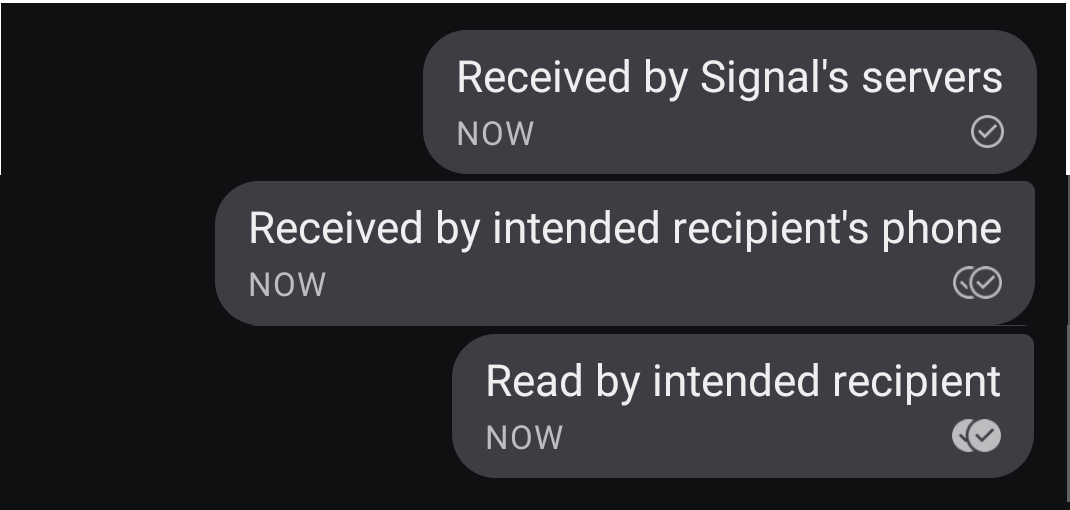
\includegraphics[width=0.8\linewidth]{figs/message-stages.png}
    \caption{\textbf{Stages of a Signal Message}\,---\,% 
        User Interface indicating message delivery status.
        % 
        One hollow check mark signifies that the message is en route. 
        %
        Two hollow check marks signifies the receipt of a delivery receipt for the message.
        %
        Finally, two filled check mark signifies the receipt of a read receipt for the message.
        %
    }
    \label{fig:signal-message-stages}
\end{figure}
}

\newcommand{\DeliveryTimeCDF}{
    \begin{figure}[t]
        \centering
        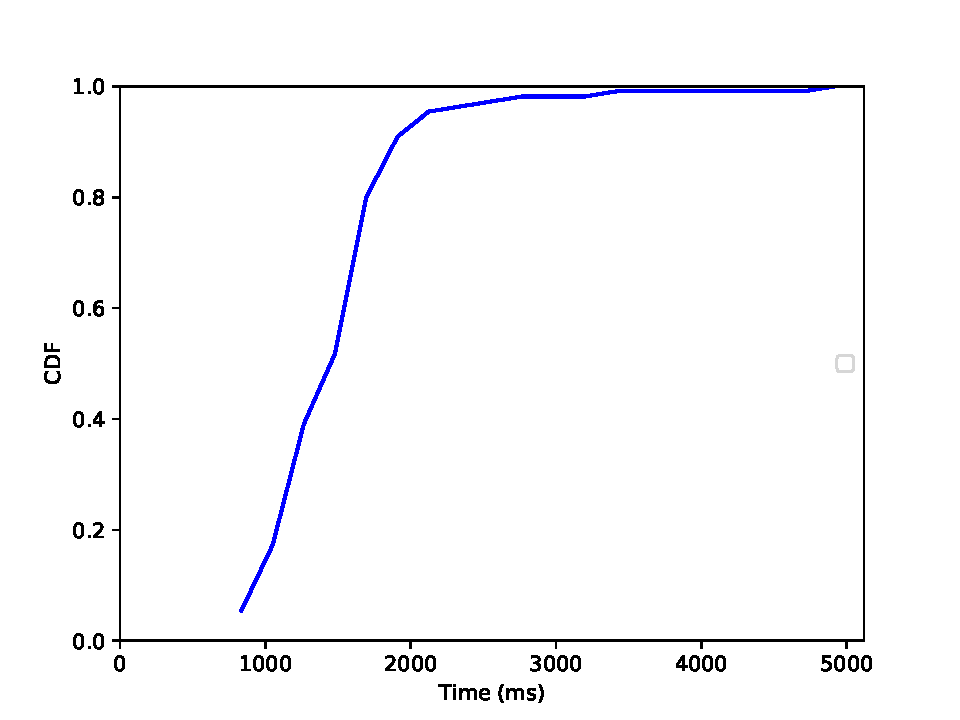
\includegraphics[width=0.8\linewidth]{figs/DRCDF.pdf}
        \caption{\textbf{CDF of Delivery Receipt timing}\,---\,%
        CDF of time between a device sending a message (to another online
        device) and receiving a Delivery Receipt. The median time is 1480ms and
        90\% of Delivery Receipts were received within 1909ms.
        }
        \label{fig:signal-delivery-cdf}
    \end{figure}
}

\newcommand{\EpochEffect}{
\begin{figure}[t]
    \centering
    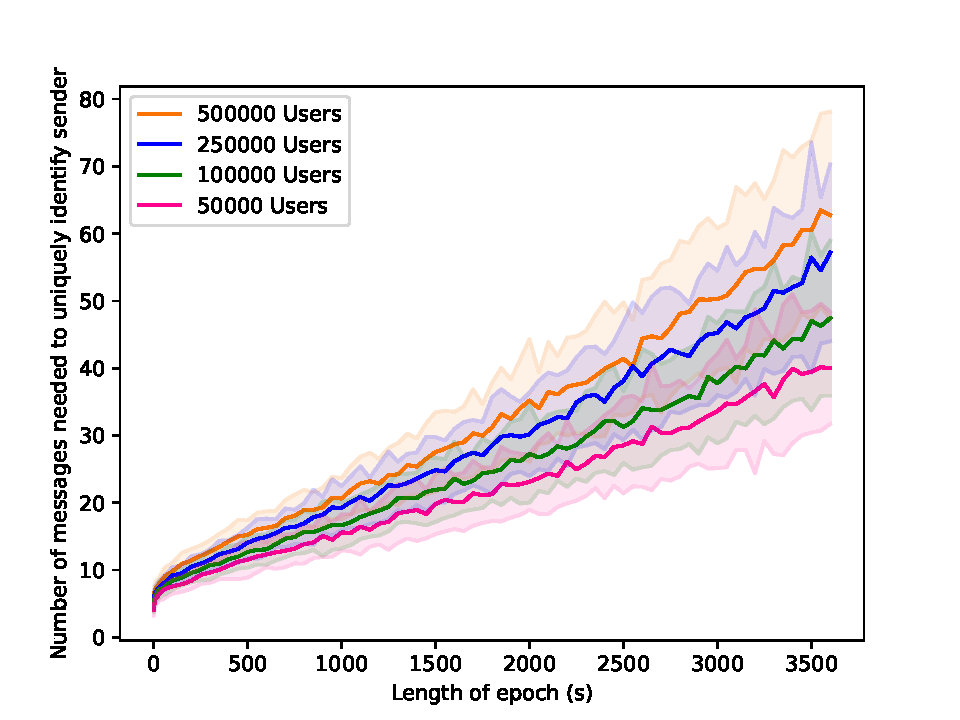
\includegraphics[width=0.9\linewidth]{figs/epoch_effect-bars.pdf}
    \caption{\textbf{Effect of delayed Read Receipts}\,---\,% 
        The attack assumes that each epoch lasts one second, and thus the log
        collects all delivery receipts that are sent within 1 second of Bob 
        receiving a sealed sender message. A possible simple solution to this
        attack is to delay (randomly per message, or publishing read receipts in
        batches) read receipts. We tested the effectiveness of the attack with
        variably sized epochs and determined that if delivery receipts were
        delayed a full hour (making them effectively worthless for their
        purpose) that with a user base of 500,000 users (each sending 50
        messages a day) Bob would need to receive 60 messages from the victim
        user to identify Alice as the sender.
        }
    \label{fig:signal-epoch-effect}
\end{figure}
}

\newcommand{\ListVsC}{
\begin{figure}[ht]
    \centering
    \includegraphics[width=0.9\linewidth]{figs/list_vs_graph.png}
    \caption{\textbf{Comparison between Python List model and Generated Graph
        Models}\,---\,% 
        After determining that the structure of the userbase graph had no effect
        on the simplified base attack (Figure~\ref{fig:NumMessages}) we modified
        our attack using Python to use a complete graph for the user base (any
        user might message any other user) and measure the effect of how
        receipts are generated for the log. In the simplified base attack the
        receipts in each epoch are structured to be 50\% random receipts, 25\%
        to be repeated receipts from a previous epoch, and 25\% receipts
        generated from replies to messages from previous epochs. As the nature
        of this attack is to only examine the `To' field of the message we
        expected only the 25\% of receipts that are repeated receipts to have
        any effect on the attack. As such we modeled our Python version to only
        have a delivery receipt from Bob to Alice and the 25\% repeated receipts
        from a previous epoch and compared to our previous models and found that
        the simplified Python model was a near match.
    }
    \label{fig:signal-listVsC}
\end{figure}
}

\newcommand{\PercentageEffect}{
\begin{figure}[t]
    \centering
    \includegraphics[width=0.9\linewidth]{figs/percentage_effect.png}
    \caption{\textbf{Effect of varying the percentage of messages in an Epoch
        that are repeated receipts}\,---\,% 
        We measured the effect of varying what percentage of an epoch's messages
        are repeated receipts from a previous epoch. As expected the larger the
        percentage, more messages persist in the recurring intersection and as
        such the attack requires more messages to identify Alice as the sender
        to Bob.
    }
    \label{fig:signal-percentageEffect}
\end{figure}
}

\newcommand{\PercentileGraph}{
\begin{figure}[ht]
    \centering
    \includegraphics[width=0.9\linewidth]{figs/Alice_percentile.pdf}
    \caption{\textbf{Alice's Percentile rank after $N$ messages}\,---\,% 
        In the full attack the number of times each user shows up in the 'To:'
        field of a Sealed Sender message in the epoch following Bob receiving a
        message is tracked. This Counter can be used to determine who is most
        likely the user in conversation with Bob. After each epoch the attacker
        can look at which users have received a message (or receipt or Typing
        Notification) most often shortly after Bob received a message. This
        graph shows Alice's precentile rank after $N$ messages---the percentage
        of users she is more likely than to be the user conversing with Bob.
    }
    \label{fig:signal-AlicePercentile}
\end{figure}
}

\newcommand{\LikelihoodGraphOld}{
\begin{figure}[ht]
    \centering
    \includegraphics[width=0.9\linewidth]{figs/Likelihood_Alice.pdf}
    \caption{\textbf{Likelihood of guessing Alice is the sender}\,---\,% 
        The natural candidate for who is messaging Bob is the user who shows up
        most often in the epoch following Bob receiving a message. This graph
        analyzes the likelihood that the attacker will be correct if they guess
        the user who has show up most often is conversing with Bob as a function
        of the number of messages Bob has received.
    }
    \label{fig:signal-AliceLikelihoodOld}
\end{figure}
}

\newcommand{\RankGraph}{
\begin{figure}[t]
    \centering
    \includegraphics[width=0.9\linewidth]{figs/Alice_rank_receipt_response_rate.pdf}
        \caption{\textbf{Number of users with Alice's count or higher after $N$ messages}\,---\,% 
        In Attack~2, we count the number of times a user receives a message in the epoch
        immediately following a message sent to Bob. This graph shows the number of users that
        have the same or higher count as Alice (the ``true'' sender in our simulation) as more
        messages are sent. We vary the percent ($f$) of epochs that send responses to Alice,
        to represent the fraction $(1-f)$ of epochs that are e.g. typing notifications or others users' messages to Bob.
        This graph effectively shows the anonymity set that Alice resides in as she
        and others send more messages to Bob, eventually shrinking down to a set of just Alice.
    }
    \label{fig:signal-AliceRank}
\end{figure}
}


\newcommand{\AttackOverview}{
\begin{figure}[t]
    \centering
    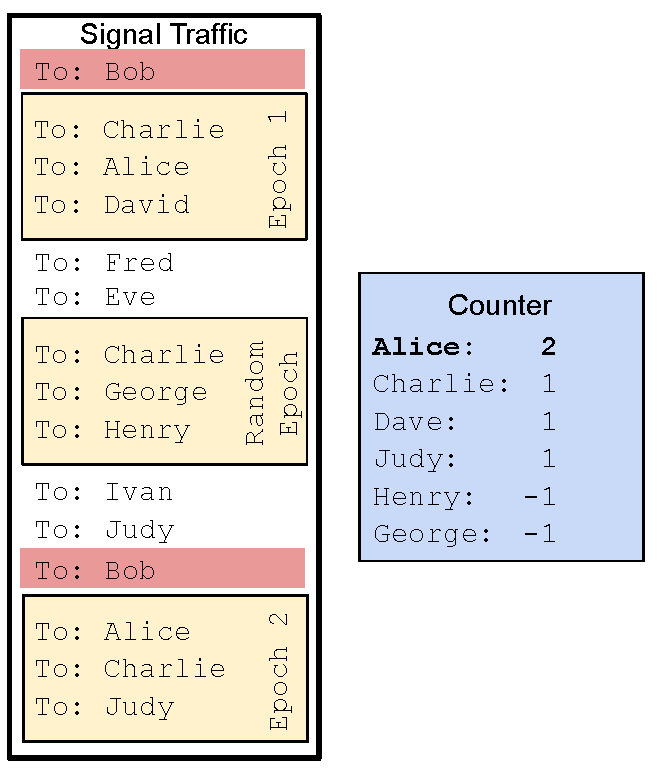
\includegraphics[clip, width=0.5\linewidth]{figs/AttackOverview.pdf}
        \caption{\textbf{Attack Overview}\,---\,% 
        Our SDA variant has the service provider (Signal) keep count of all
        users who receive messages in the \textit{epoch} after Bob receives a
        message to determine who is consistently messaging at the same time as
        Bob is receiving a message. Additionally, the service provider will
        begin an epoch at a random time to keep track of users which are
        messaging independent of the associates of Bob, and those users will be
        deducted from the counter. As such, ``popular'' users such as
        \textit{Charlie} will not mask Alice's behavior.
    }
    \label{fig:signal-AttackOverview}
\end{figure}
}

\newcommand{\LikelihoodGraph}{
\begin{figure}[t]
    \centering
    \includegraphics[width=0.9\linewidth]{figs/likelihood_receipt_response_rate.pdf}
    \caption{\textbf{Likelihood of guessing Alice is the sender}\,---\,% 
        The natural candidate for who is messaging Bob is the user who shows up
        most often in the epoch following Bob receiving a message. This graph
        analyzes the likelihood that the attacker will be correct (i.e. they will pick Alice)
        if they guess the user who has show up most often is conversing with Bob as a function
        of the number of messages Bob has received. Simulated over 1000 randomized iterations.
    }
    \label{fig:signal-AliceLikelihood}
\end{figure}
}

\newcommand{\SealedSenderStructure}{
\begin{figure}[ht]
    \centering
    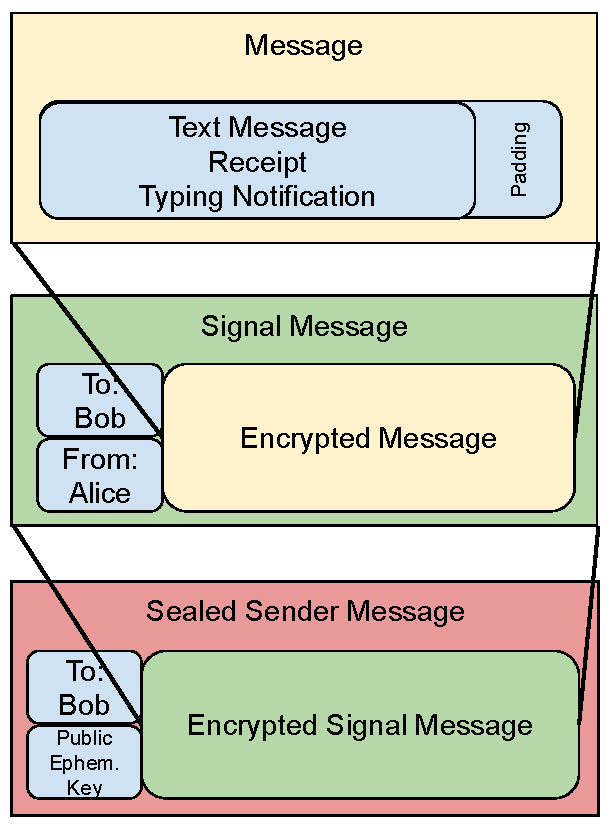
\includegraphics[width=0.5\linewidth]{figs/SealedSenderStructure.pdf}
    \caption{\textbf{Structure of Signal Messages}\,---\,% 
        All messages Alice sends to Bob through Signal (receipts, text messages,
        or events) are first padded to the next multiple of 160 bytes. The
        padded message is then encrypted under the shared key between Alice and
        Bob and then combined with `To: Bob' and `From: Alice' metadata to form
        a Signal Message. %If either Bob or Alice do not have sealed sender enabled this Signal Message will then be sent.
        If both Alice and Bob
        have sealed sender enabled then Alice will then generate an ECDHE key
        pair and derive a new shared secret with Bob's public key to encrypt
        the Signal Message and combine with `To: Bob' and the public ephemeral
        key to form a sealed sender message that will be sent to Bob.
    }
    \label{fig:signal-SealedSenderStructure}
\end{figure}
}

\newcommand{\VariantThree}{
\begin{figure}[ht]
    \centering
    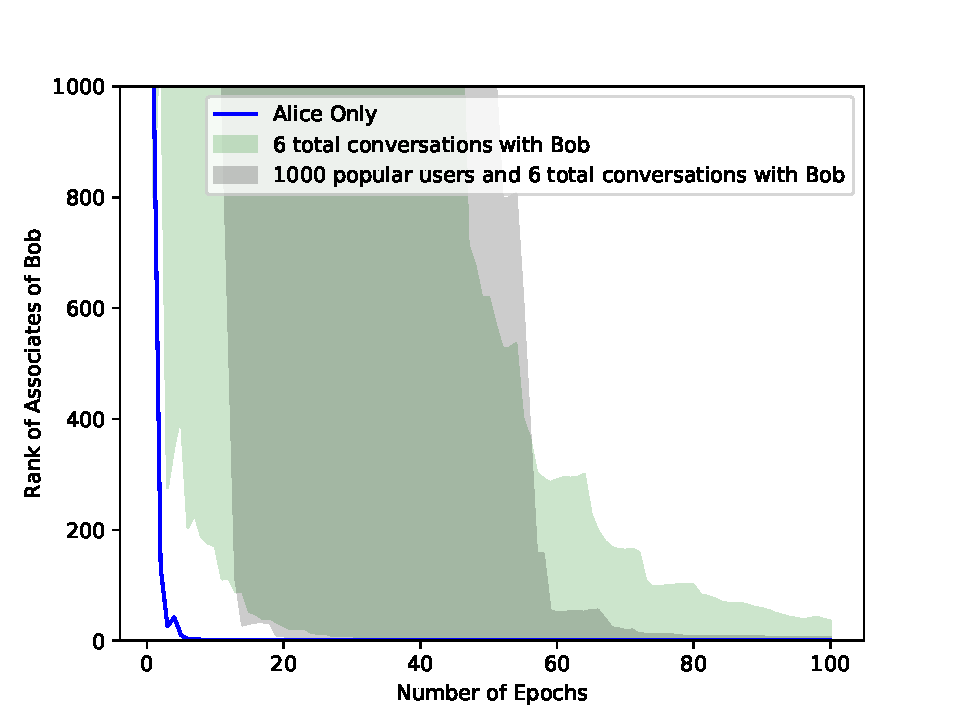
\includegraphics[width=0.9\linewidth]{figs/various_cases.pdf}
    \caption{\textbf{Effect of popular users}\,---\,% 
        We examined the effectiveness of our SDA by examining the cases where
        only Alice is messaging Bob and where Bob is being messaged by Alice and
        5 other users. The graph shows the rank of those messaging Bob, how many
        users have received more messages than those messaging Bob. When only
        Alice is messaging Bob each of the attack epochs are started by her,
        meaning her rank will very quickly drop. When multiple users are
        messaging Bob there is a range of ranks, represented by the green band
        which demonstrates the lowest ranked user messaging Bob (on the bottom)
        and the highest ranked individual messaging Bob (on the top). When
        epochs are begun by multiple users, an individual's rank takes a while
        to drop. The graph shows that for over 45 epochs one of the users
        messaging Bob has a rank of over 1000, while another user messaging Bob
        has dropped to a rank of 0 (meaning they have received a message after
        Bob received a message the most of any user in the system).
    }
    \label{fig:signal-variant3}
\end{figure}
}


\newcommand{\combinedfigures}{
\begin{figure*}[t]

    \centering
    \begin{minipage}{0.49\textwidth}
        \centering
    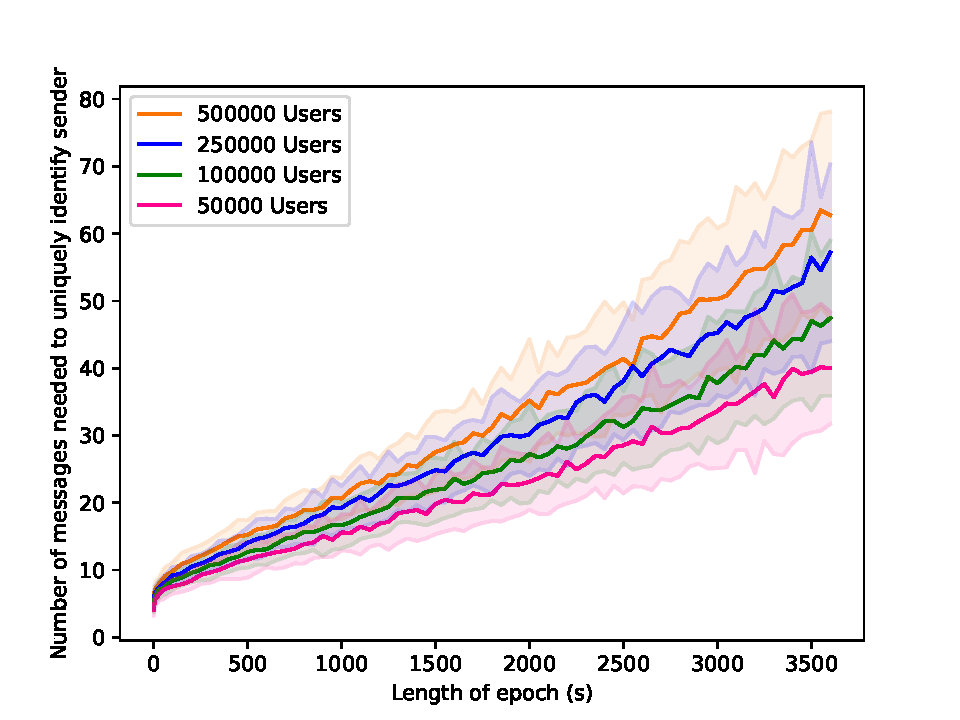
\includegraphics[width=\linewidth]{figs/epoch_effect-bars.pdf}
    \end{minipage}\hfill
    \begin{minipage}{0.49\textwidth}
        \centering
    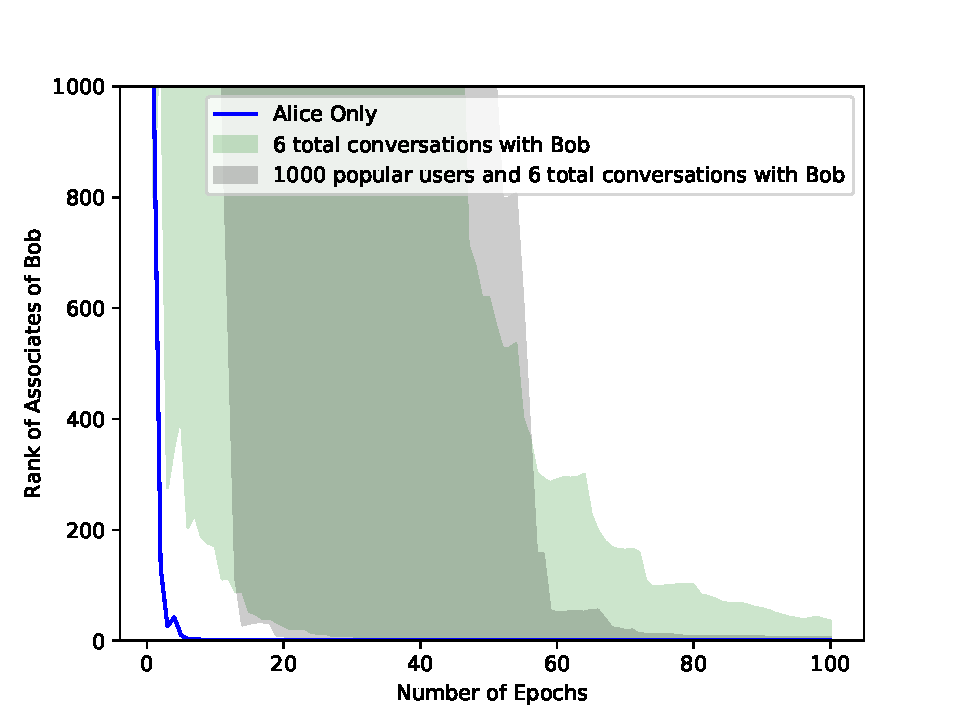
\includegraphics[width=\linewidth]{figs/various_cases.pdf}
    \end{minipage}

%     \begin{minipage}[width=0.5\linewidth]
%     \centering
%     \includegraphics[width=0.9\linewidth]{figs/epoch_effect.pdf}
%     \end{minipage}

%     \begin{minipage}[width=0.5\linewidth]
%     \centering
%     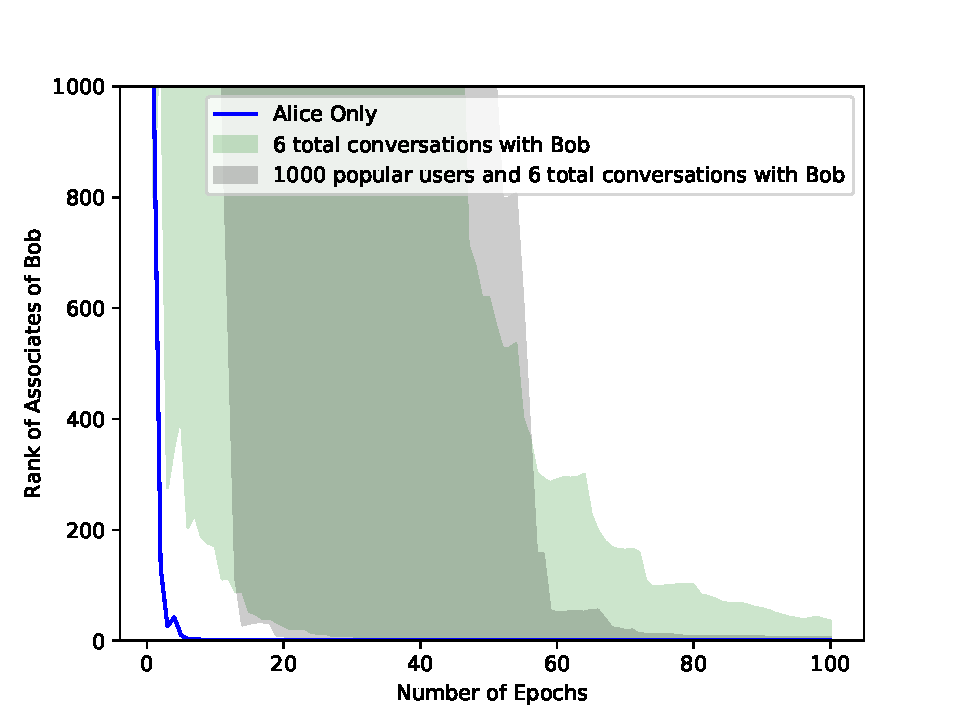
\includegraphics[width=0.9\linewidth]{figs/various_cases.pdf}
%     \end{minipage}


    \caption{\textbf{Left: Effect of delayed Read Receipts}\,---\,% 
        The attack assumes that each epoch lasts one second, and thus the log
        collects all delivery receipts that are sent within 1 second of Bob 
        receiving a sealed sender message. A possible simple solution to this
        attack is to delay delivery receipts.
        We tested the effectiveness of the attack with
        variably sized epochs and determined that if delivery receipts were
        delayed a full hour (making them effectively worthless for their
        purpose) that with a user base of 500,000 users (each sending 50
        messages a day) Bob would need to receive 60 messages from the victim
        user to identify Alice as the sender. \\
        \textbf{Right: Effect of popular users in our SDA}\,---\,% 
        We examined the effectiveness of our SDA variant by examining the cases
        where only Alice is messaging Bob and where Bob is being messaged by
        Alice and 5 other users. The graph shows the rank of those messaging
        Bob, how many users have received more messages than those messaging
        Bob. When only Alice is messaging Bob each of the attack epochs are
        started by her, meaning her rank will very quickly drop. When multiple
        users are messaging Bob there is a range of ranks, represented by the
        green band which bounds the lowest ranked user messaging Bob (on
        the bottom) and the highest ranked individual messaging Bob (on the
        top). When epochs are begun by multiple users, an individual's rank
        takes a while to drop. The graph shows that for over 45 epochs one of
        the users messaging Bob has a rank of over 1000, while another user
        messaging Bob has dropped to a rank of 0 (meaning they have received a
        message after Bob received a message the most of any user in the
        system). The black band considers the same situation, but with 1000 popular users in the system which our variant accounts for.
        }
    \label{fig:signal-combinedfigure}
\end{figure*}
}


%%% Local Variables:
%%% mode: latex
%%% TeX-master: "main"
%%% End:


% \newcommand{\oldattacktext}{}

%
\chapter{Improving Signal's Sealed Sender}\label{ch:signal}


% \makeatletter
% \newcommand{\linebreakand}{%
%   \end{@IEEEauthorhalign}
%   \hfill\mbox{}\par
%   \mbox{}\hfill\begin{@IEEEauthorhalign}
% }
% \makeatother

% % author names and affiliations
% % use a multiple column layout for up to three different
% % affiliations
% \IEEEoverridecommandlockouts

% \author{
% \IEEEauthorblockN{Ian Martiny\IEEEauthorrefmark{1}, Gabriel Kaptchuk\IEEEauthorrefmark{2}, Adam Aviv\IEEEauthorrefmark{3}, Dan Roche\IEEEauthorrefmark{4}, Eric Wustrow\IEEEauthorrefmark{1}}
% \IEEEauthorblockA{\IEEEauthorrefmark{1}University of Colorado Boulder, 
% \{ian.martiny, ewust\}@colorado.edu}
% \IEEEauthorblockA{\IEEEauthorrefmark{2}Boston University, 
% kaptchuk@bu.edu}
% \IEEEauthorblockA{\IEEEauthorrefmark{3}George Washington University, 
% aaviv@gwu.edu}
% \IEEEauthorblockA{\IEEEauthorrefmark{4}U.S. Naval Avademy, 
% roche@usna.edu}
% % \IEEEauthorblockN{Ian Martiny}
% % \IEEEauthorblockA{University of Colorado Boulder\\
% % ian.martiny@colorado.edu}
% % \and
% % \IEEEauthorblockN{Gabriel Kaptchuk}
% % \IEEEauthorblockA{Boston University\\
% % kaptchuk@bu.edu}
% % \and
% % \IEEEauthorblockN{Adam Aviv}
% % \IEEEauthorblockA{George Washington University\\
% % aaviv@gwu.edu}
% % \linebreakand
% % \IEEEauthorblockN{Dan Roche}
% % \IEEEauthorblockA{U.S. Naval Avademy\\
% % roche@usna.edu}
% % \and
% % \IEEEauthorblockN{Eric Wustrow}
% % \IEEEauthorblockA{University of Colorado Boulder\\
% % ewust@colorado.edu}
% }



% \makeatletter\def\@IEEEpubidpullup{6.5\baselineskip}\makeatother
% \IEEEpubid{\parbox{\columnwidth}{
%     Network and Distributed Systems Security (NDSS) Symposium 2021\\
%     21-24 February 2021\\
%     ISBN 1-891562-66-5\\
%     https://dx.doi.org/10.14722/ndss.2021.23180\\
%     www.ndss-symposium.org
% }
% \hspace{\columnsep}\makebox[\columnwidth]{}}

% % make the title area
% \maketitle



% \begin{abstract}
%  \abstract{  \OnePageChapter	% because it is very short
	The vast majority of online services are run using a centralized
	infrastructure. The centralized nature of these services allow the provider
	to have absolute control over the content as well as any profit generated by
	that content. Centralized services often have servers distributed across the
	world for user reliability, though they function as centralized systems:
	their functionality is identical across their network and the data they
	collect is available to the service as a whole, not only the server a user
	interacts with. Users of these services, and the data they generate, are
	completely at the whim of the provider; companies often offer vague promises
	of security and privacy of the data collected from their users which the
	users cannot verify themselves. Moving these services to a decentralized
	system (where each server acts independently of others) could address these
	issues but decentralized systems often face severe scalability issues as
	well as having cumbersome requirements on users such as needing specialized
	software to access the service.

    This dissertation demonstrates that user privacy can be inherently built
    into centralized systems using cryptographic protocols. Centralized systems
    can offer their services with minimal user information allowing services
    \emph{actually} geared towards privacy to have it be a core functionality of
    their service. A service that doesn't have access to users data cannot abuse
    or leak it.

    \emph{Proof of Censorship} utilizes Private Information Retrieval to allow
    content providers (such as Twitter) to be cryptographically auditable over
    whether content has been modified or removed. In 2018 Signal (a secure
    end-to-end messenger) introduced Sealed Sender in an attempt to hide the
    sender of encrypted messages. \emph{Improving Signal's Sealed Sender}
    strengths Sealed Sender by guaranteeing that privacy cryptographically using
    blind RSA signatures. \emph{Mind the IP Gap} measures how countries utilize
    their centralized censorship apparatus to restrict content to users through
    DNS manipulation. 

	}
% \end{abstract}

\section{Introduction} % basic introduction, problem statement etc

Secure end-to-end encrypted messaging applications, such as Signal,
protect the content of messages between users from potential eavesdroppers using
protocols like off-the-record (OTR) messaging \cite{BGB04,
DiRaimondo:2005:SOM:1102199.1102216}. These protocols guarantee that even the
service provider itself is unable to read communication between users. However,
these protocols do not protect conversation \emph{metadata}, including sender,
recipient, and timing.  For instance, if Alice sends a message to Bob, the
server will learn that there is a relationship between those two users and when
they communicated.

\medskip
\noindent
\textbf{Protecting metadata.} While leaking metadata may appear reasonable when compared to revealing the contents of the messages,
observing metadata can have serious consequences. Consider that Alice may be a whistleblower communicating with a journalist
\cite{190976} or a survivor of domestic abuse seeking confidential support
\cite{236244}. In these cases, merely knowing \emph{to whom} Alice is communicating combined with other contextual information is often enough to infer
conversation content without reading the messages themselves. Former NSA and CIA director Michael Hayden succinctly illustrated this importance of metadata when he said the US government ``kill[s] people based on metadata'' \cite{haydenmetadata}.

% In fact, Paul
% Revere's revolutionary tendencies can be identified from the metadata of what
% organizations he and other colonists were members of~\cite{healy_2013}.

Signal's recent \emph{sealed
sender} feature aims to conceal this metadata by hiding the message sender's identity.
Instead of seeing a message from Alice to
Bob, Signal instead observes a message to Bob from an anonymous sender. This message
can only be decrypted by Bob, who then learns from the payload that the message
originated with Alice. Ideally, using the sealed sender protocol breaks the link
between the sender and the receiver, preventing Signal from recording 
sender-recipient pairs, if ever compromised or compelled to do so.

While sealed sender is currently only deployed by Signal, Signal's design decisions
are highly influential for other secure messaging platforms as it is a leader in 
deploying cutting-edge secure messaging features; the Signal protocol has 
been integrated into other services like WhatsApp.  Understanding and  uncovering flaws
in sealed sender is therefore not only important to protecting the privacy of Signal's
millions\footnote{Signal does not publicly disclose its user count, but the app has been downloaded millions of times.}
 of users \cite{signalusercount}, but also helps make sure sealed sender fully realizes
its goal before it is integrated into other services with other sets of users.
%and even with
%While Signal still learns some metadata about the information, having only a recipient
%makes interpreting this message, even with other contextual information,
%significantly more difficult.

\medskip
\noindent
\textbf{A new SDA on message timings.}
We present a new statistical disclosure attack (SDA) applicable to messages in Signal's sealed sender, that
would allow the Signal service---if compelled by a government or compromised---to correlate
senders and receivers even when using the sealed sender feature.
Previously,
\emph{statistical disclosure
attacks} (SDAs) have been studied since the 2000s to
link senders and recipients in anonymous mix
networks~\cite{SDA,SDA-MD05,LSDA,two-sided-SDA,reverse-SDA}.
%infer information about sender-recipient correlations after viewing a large volume of
%traffic in and out of a mix network (\cite{SDA,SDA-MD05,LSDA}).
These attacks work by correlating sender and receiver behavior across multiple rounds of the mix.


It is not immediately obvious how SDAs could be applied in the context
of sealed sender messages, since there is no mix network and the identities of
senders are (by design) never revealed. Thus, it is not clear how even the server
could apply SDA attacks, since it only learns the destinations of messages, and
never sources.

%In traditional (encrypted) messaging without sealed sender, SDAs have no
%relevance since the sender/recipient identities are already revealed to
%the server. But in the presence of sealed sender, it is not obvious how
%such attacks could be applied, since there is no mix network and the
%identities of parties sending messages at any moment are (by design) not
%revealed to the server.

In this paper, we observe that, \emph{by assuming that most messages
receive a quick response}, we can overcome these seeming limitations of
sealed-sender messaging and employ a SDA-style attack to
de-anonymize sender-recipient pairs after passively observing enough messages.
%(Note, a similar assumption, in the context of mix
%networks, was used by \cite{two-sided-SDA,reverse-SDA}.)

Moreover, and crucially, \emph{this quick-response assumption is guaranteed to be true
in the presence of delivery receipts}, a feature of Signal's
current implementation that cannot be disabled by the user.
When Alice sends Bob a sealed sender message, Bob's device will
automatically generate a delivery receipt that acknowledges Alice's message. Although
this delivery receipt is also sent via sealed sender to Alice, the predictability of its timing makes our attack more effective.

The differences between sealed sender messaging and a general mix network allow
us to develop a simple, tailored SDA-style attack, using ideas similar to
\cite{SDA-MD05},
which can be used to de-anonymize a conversation between two parties.
Compared to prior work, our attack is more limited in scope, but is also
more efficient: it runs in linear-time in the amount of traffic
observed, and we prove that the probability our attack succeeds increases exponentially with the number of observations.

%derive a simple, exponentially-decreasing lower
%bound on the probability of de-anonymizing the conversation as a function of the number of
%observations.

\if0
We also validate our attack with simulations,
demonstrating that under reasonable circumstances, a conversation can be
de-anonymized in fewer than 60 observations.

\medskip
\noindent
\textbf{A new timing attack.\todo{remove this part}} In this paper, we show that there exists a novel timing attack on Signal's sealed sender protocol that allows a network observer to efficiently identify the pairs of users that are communicating. This demonstrates that sender anonymity of sealed sender does not compose over a conversation of multiple messages back and forth.
%with back and forth communication, even if both parties are using sealed sender. This is due to a novel timing attack.

Our key observation is that while Signal only sees the recipient of sealed sender 
messages, the timestamps of these messages still leak critical information.  As Alice 
and Bob continue a conversation (beyond the initial message), the timing information can be enough to link Alice to Bob, even if both parties are using sealed sender.  That is, an observer can learn that Alice engaged (and initiated) a conversation with Bob with high confidence. 


The timing attack is made worse by Signal's default setting of delivery receipts. When Alice sends Bob a sealed sender message, Bob's device will
automatically generate a delivery receipt that acknowledges Alice's message. Although
this delivery receipt is also sent via sealed sender to Alice, the predictability of its timing makes our attack more effective.
\fi

\medskip
We validate the practicality of the timing attack in two ways. First,
using a probabilistic model of communication, we prove a bound on
the probability that Alice can be identified as communicating with Bob
after a finite number of messages, independent of other users' activity.
The probability also scales logarithmically with the number of active users.

Second, we run simulations to estimate the effectiveness of the attack in practice. In the most basic simulation, Alice can be uniquely identified as communicating with Bob after fewer than 10 messages. We also add complicating factors such as
multiple simultaneous conversations with Alice and/or Bob and
high-frequency users in the system, and show that these delay but do not
prevent Alice from being de-anonymized.
% simulation. We show that even with significant
% other sealed sender activity on the network, given enough message pairs, Signal is able
% to uniquely identify Alice and Bob. The activity on the network, such as highly popular users communicating frequently with multiple partners, increased the burden on the attacker, but only delays the reidentification  attack. We estimate, that only a few dozen sealed sender messages, is sufficient in most settings to identify communicating parties. \adam{this paragraph needs to be updated with new simulation results}


% This will appear as a sealed sender message to Bob, followed shortly by a sealed sender message to Alice. If these two messages can be linked together,
% Signal will learn that Alice and Bob are communicating.



\medskip
\noindent
\textbf{Sealed sender conversations.} To fix this problem, we
provide a series of practical solutions that require only modest changes to Signal's
existing protocol.
We first define a simulation-based security model for sealed sender \emph{conversations}
(rather than just single messages) that allows the original recipient of the
sealed sender message to be leaked but never the initiator of that message
(sender)
through the lifetime of the conversation. We then present three solutions that
accomplish the goal of sealed sender conversations. Each is based on ephemeral
identities, as opposed to communicating with long-term identifiers, such as the keys linked to your phone number in Signal. Each additional solution provides additional security protections.

Our first solution provably provides {\em one-way sealed-sender} conversations, a new security guarantee for which we provide a formal, simulation based definition. In this protocol, Alice %, a sender wishing to remain anonymous,
initiates a sealed-sender conversation by generating a new ephemeral, public/secret key and anonymously registers the ephemeral public key with an anonymous mailbox via the service provider. Alice then uses a normal sealed sender message to the receiver Bob to send the anonymous mailbox identifier for his replies.  Alice can retrieve Bob's replies sent to that anonymous mailbox by authenticating with her ephemeral secret key,
and the conversation continues using traditional sealed sender messages between Bob's long-term identity and the anonymous mailbox Alice opened.
%and further communication within the conversation from Alice to Bob uses traditional sealed sender, but all replies from Bob to Alice is sent via the anonymous mailbox.

We show that this solution can be further enhanced if both Alice and Bob use ephemeral identities, after the initial message is sent (using sealed sender) to Bob's long-term identity.
% This solution can then extended for {\em two-way sealed-sender} communication. As before, Alice registers an anonymous mailbox and send the mailbox identifier to Bob using a sealed-sender message.  Then, {\em Bob} also registers an anonymous mailbox upon receiving the initiation message. Bob replies to Alice's initial message via a sealed sender message to Alice's anonymous mailbox, and within the envelope is the address of Bob's anonymous mailbox. Further communication between the parties continues via sealed sender message to each other's anonymous mailbox.
This protocol provides both sender and receiver anonymity for the length of a conversation if the server is unable to correlate Bob's receipt of the initial message and his anonymous opening of a new mailbox, meaning the server has only one chance to deanonymize Bob.    Importantly, even if the server is able to link these two events, this extension still (provably) provides {\em one-way sealed-sender}.

Neither of the above solutions offer authentication of anonymous mailboxes at
the service provider, e.g., Signal.  A malicious user could open large numbers
of anonymous mailboxes and degrade the entire system.
% Because any user may open any number of anonymous mailboxes, this could
% degrading service, particularly if there are malicious users.
We offer an overlay solution of {\em blind-authenticated anonymous mailboxes}
for either one-way or two-way sealed-sender conversations whereby each user is
issued anonymous credentials regularly (e.g., daily) that can be ``spent''
(verified anonymously via a blind signatures) to open anonymous new mailboxes.
To evaluate the practicality of using anonymous credentials in this way, we run
a series of tests to compute the resource overhead required to run this overlay.
We estimate that running such a scheme on AWS would cost Signal approximately
\$40 each month to support 10 million anonymous mailboxes per day.



% However, we acknowledge that this solution would still require a
% significant engineering effort to fully integrate with the Signal
% protocol. To that end, we also discuss a number of simple strategies
% which could be deployed immediately in order to largely prevent the
% attacks we have demonstrated.

\medskip
\noindent
\textbf{Our contributions.} In this paper, we will demonstrate
\begin{itemize}[nosep]
  \item A brief analysis of how the Signal protocol sends messages and
    notifications based on source code review and instrumentation
    (\cref{sec:signal-message-types});
  \item The first attack on sealed sender to de-anonymize the initiator of a conversation in Signal (\cref{sec:signal-attack});
  \item Validation of the attack via theoretical bounds and simulation models (\cref{sec:signal-attack-eval});
  \item A new security model that defines allowed leakage for sender-anonymous communication;
  \item A set of increasingly secure solutions, that are either one-way anonymous, two-way anonymous, and/or provide anonymous abuse protections. (\cref{sec:signal-solution});
  \item An evaluation of the resource overhead introduced by using blind signatures to prevent anonymous mailbox abuse, and estimates of its
    effective scalability to millions of users (\cref{sec:signal-impl}); and
  \item Immediate stopgap strategies for Signal users to increase the difficulty of our attack (\cref{sec:signal-othersolutions}).
\end{itemize}
\vspace{4pt}

We include related work and the relevant citations in \cref{sec:signal-related_work}.  We also want to be clear about the limitations of our work and its implications:
\begin{itemize}[nosep]
  \item We do \emph{not} consider network metadata such as leakage due
    to IP addresses. See \cref{sec:signal-threat} and the large body of existing
    work on anonymizing proxies such as Tor.
  \item We do \emph{not} consider messaging with more than two parties,
    i.e.\ group messaging. This is important future work; see the
    discussion in \cref{sec:signal-group}.
  \item Our attack does \emph{not} suggest that Signal is less secure
    than alternatives, or recommend that users discontinue using it.
    Other messaging services do not even attempt to hide
%     Indeed, our attacks would apply to other messaging services but are
%     most relevant to the Signal protocol as it actually attempts to hide
    the identities of message senders.
  \item We do \emph{not} believe or suggest that Signal or anyone else is using this attack
          currently.
  \item While we have implemented the core idea of our solution in order
    to estimate the cost of wider deployment, we have \emph{not}
    undergone the serious engineering effort to carefully and correctly integrate this
    solution with the existing Signal protocol software in order to
    allow for practical, widespread deployment.
\end{itemize}
\vspace{4pt}

\noindent
\textbf{Responsible Disclosure.} We have notified Signal of our attack and solutions prior to publication, and Signal has acknowledged our disclosure.
%Simultaneously with the submission of this manuscript, we have responsibly disclosed this attack to Signal.

%%% Local Variables:
%%% mode: latex
%%% TeX-master: "main"
%%% End:

\section{Background}\label{sec:Signal-background}

% Although many protocols have been suggested for sending end-to-end
% encrypted messages (see \cref{sec:relwork-msging}), the most commonly
% used in practice for mobile messaging is the Signal protocol~\cite{Mar13},
% currently used by both the Signal and WhatsApp applications. 

We now give
some background on the structure and types of messages in the Signal protocol~\cite{Mar13}, used in both the Signal and WhatsApp applications.

\subsection{Sealed Sender Messages} % what is signal, what is sealed sender
\label{ssec:signal-signal}
Although % the protocols used by
secure end-to-end encrypted messaging %(SEEM)
applications like Signal protect the
contents of messages% sent between users
, they reveal metadata about
\emph{which} users are communicating to each other. In an attempt to hide this
metadata, Signal recently released a feature called sealed
sender~\cite{sealed-sender} that removes the sender from the metadata
intermediaries can observe.

To send a sealed sender message to Bob, Alice connects to the Signal server and
sends an encrypted message to Bob anonymously\footnote{As we note in our threat
model, we do not consider the information leakage from networking.}. Within the
payload of this encrypted message, Alice includes her own identity, which allows
Bob to authenticate the message.  Importantly, Signal still learns Bob's
identity, which is needed in order to actually deliver it. %; without this identity, Signal cannot deliver the message.
The structure of sealed sender messages are illustrated in \cref{fig:signal-SealedSenderStructure}.

Due to sender anonymity,
Signal cannot directly rate-limit users to prevent spam or abuse.  Instead,
Signal derives a 96-bit \emph{delivery token} from a user's profile key, and
requires senders demonstrate knowledge of a recipients' delivery token to send
them sealed sender messages.
% For instance, to send a sealed sender message to
% Bob, Alice must have knowledge of his delivery token.
By only sharing this delivery token with his contacts, Bob
limits the users who can send him sealed
sender messages, thus reducing the risk of abuse\footnote{There are a number of
options available to Bob that can allow more fine-grained access control to his
delivery token.  Bob can opt to receive sealed sender messages from anyone even
without knowledge of his delivery token, but this is disabled by default.
Additionally, Bob can regenerate his delivery token and share it only with a
subset of his contacts to block specific users.}.

\subsection{Types of Messages}
\label{sec:signal-message-types}

We manually reviewed and instrumented the Signal messenger Android
4.49.13 source code~\cite{signal-source} in order to understand the types of
messages Signal sends. In addition to the messages that contain content to be
delivered to the receiver, there are several event messages that can be sent
automatically, as discussed below. All of these messages are first padded to the
next multiple of 160 bytes, then encrypted and sent using sealed sender (if
enabled), making it difficult for the Signal service to distinguish events from
normal messages based on their length. %Figure~\ref{fig:SealedSenderStructure}
%shows the structure of sealed sender messages, and Figure~\ref{fig:message-stages}
%shows the user interface for each stage of message acknowledment in Signal.

\SealedSenderStructure

\MessageStages

\medskip \noindent
\textbf{Normal message.}
A normal text message or multimedia image sent from Alice to Bob is the
typical message we consider. A short (text) message will be padded to
160 bytes, and longer messages padded to a multiple of 160 bytes, before
encryption.
% could cut?
%While the application UI displays a stream of messages
%between Alice and Bob in a single window as a conversation, in the
%protocol there is no distinction between the first or any subsequent
%messages in a given conversation.


\medskip \noindent
\textbf{Delivery receipt.} 
When Bob's device \emph{receives} a normal message, his device will
automatically send back a delivery receipt to the sender. When Alice receives
the delivery receipt for her sent message, her device will display a second
check mark on her sent message to indicate that Bob's device has received the
message (see \cref{fig:signal-message-stages}). If Bob's device is online when Alice sends her message, the delivery receipt will be sent back immediately. 
We measured a median time of 1480~milliseconds between sending a message and receiving a delivery receipt from an online device. (See Figure~\ref{fig:signal-delivery-cdf} for CDF of times.)
These receipts
{\em cannot be disabled} in Signal.
\DeliveryTimeCDF
% 90% of messages received the delivery receipt in less than 1880ms

\medskip \noindent
\textbf{Read receipt (optional).} 
Bob's device will (optionally) send a read receipt to the sender when he has \emph{viewed} a normal
message, triggering a UI update on Alice's device 
(see \cref{fig:signal-message-stages}). Unlike delivery receipts, Bob can disable read receipts. However, Alice may still send read receipts for messages she receives
from Bob. If Bob receives a read receipt but has the feature disabled, his user
interface will not display the notification. %When interacting with the UI, the
%feature will appear to be disabled for both users if Bob turns it off, although
%Alice might still be sending read receipts.

\medskip \noindent
\textbf{Typing notifications (optional).}\label{sssec:signal-typingNotifications}
Alice's device will (optionally) send a \emph{start typing} event when Alice is entering a
message, which Bob's device will use to show that Alice is typing. If she does
not edit the message for 3 seconds, a \emph{stop typing} event will be sent.
Each sent message is accompanied by a \emph{stop typing} event to clear the
receiver's typing notification. Like read receipts, typing notifications can be
disabled such that the user will not send or display received notifications.
%However, if their peer still has typing notifications enabled, their device will
%still receive (but ignore) these events.


% More intro-y than background-y
%Signal~\cite{signal} is a popular secure end-to-end encryption smartphone app
%that uses off-the-record~\cite{otr} communication to protect the contents sent
%between users. 

\subsection{Threat Model}
\label{sec:signal-threat}
% assumptions of attack, we know that a Network
% inference attack is possible no matter what, assume that messages/receipts are
% sent through Tor.

We assume that the service provider (e.g. Signal) passively monitors messages
to determine which pairs of users are communicating.  This models either an insider threat or a service provider compelled to perform surveillance in response to a government request.
We assume Alice and Bob have already exchanged delivery tokens and they communicate using sealed sender. Once initiated, we
assume that Alice and Bob will continue to communicate over time.  Finally, we also assume that
many other users will be communicating concurrently during Alice and Bob's conversation,
potentially with Alice and/or Bob.  
%\gsk{is this the
%goal?  like is the output of adv 1/0 or is it an identity bob}.

The service provider cannot view the contents of the encrypted sealed sender
messages, but knows the destination user for these messages (e.g. someone sends
a message to Bob).  We assume that Alice and Bob have verified their respective 
keys out of band,
and that the applications/devices they are using are secure.
Although the service provider publishes the application, they typically
distribute open-source code with deterministic builds, which we assume prevents
targeting individual users.

We note that the service provider could infer a sender's identity from network metadata
such as the IP address used to send a sealed sender message. However, this is a problem
that could be solved by using a popular VPN or an
anonymizing proxy such as Tor~\cite{signal-tor, tor_two}. For the purposes of
this paper, we assume that users who wish to remain anonymous to Signal can use
such proxies (e.g. Orbot~\cite{guardianproject}) when sending sealed sender messages (and, in our solution,
when receiving messages to ephemeral mailboxes), and we do not use network
metadata in our attack.

In terms of impact, we note that a recent study
suggests as many as 15\% of mobile users already use VPNs every day
\cite{vpn-usage};
this prevalence is even higher in east Asia and, presumably, among
vulnerable user populations.
%When receiving
%messages, users are unlikely to benefit from Tor, as they must authenticate to
%Signal with their
%identity to receive messages.

%%% Local Variables:
%%% mode: latex
%%% TeX-master: "main"
%%% End:


\section{Attack Description}\label{sec:signal-attack}

We will present a kind of \emph{statistical disclosure attack} (SDA)
that can be used to de-anonymize a single user's contacts after a chain
of back-and-forth messages, each of which is sent using sealed sender.

We first explain how, especially in the presence of delivery receipts, a
sealed-sender messaging system can be viewed as a kind of mix network;
this observation allows for the use of SDAs in our context and can be
viewed as one of our contributions.

Next, we detail a simple attack for our specific use-case of sealed
sender messaging, which can be viewed as a special case of an SDA attack
proposed in \cite{SDA-MD05}. 
%As we will see in the next section, by
%targeting this specific application, our attack can de-anonymize a
%single target user's contacts in many fewer rounds than existing
%SDAs in the literature.

\subsection{From mixnets to sealed-sender}

In anonymous networking, a simple \emph{threshold mix} works as follows:
When Alice wants to send a message to Bob, she instead encrypts it and
sends it to a trusted party called the \emph{mix}.
Once the mix receives messages from a certain
threshold $\tau$ number of other senders, the mix decrypts their destinations,
shuffles them, and sends all messages out to their destinations at once.
In this way, a network attacker can observe which users are sending messages and which are receiving message, but cannot easily infer which pairs of individuals are directly communicating.

The basis of SDAs, first proposed by \cite{SDA},
is that the messages sent through the mix over multiple
rounds are not independent; a user such as Alice will normally send
messages to the same associates (such as Bob) multiple times in
different rounds. In the simplest case, if Alice sends messages only to
Bob, and the other users in each round of mixing are random, then a
simple \emph{intersection attack} works by finding the unique common
destination (Bob) out of all the mixes where Alice was one of the
senders.

Over the last two decades, increasingly sophisticated variants of SDAs
have been proposed to incorporate more complex mix networks~\cite{SDA-MD05}, 
infer sender-receiver connections~\cite{reverse-SDA},
adapt to the possibility of anonymous replies~\cite{two-sided-SDA}, and
to use more powerful techniques to discover information about the entire
network topology~\cite{vida-SDA,LSDA}.
Fundamentally, these all follow a similar anonymous networking model,
where an attacker observes messages into and out of a mix network, and
tries to correlate senders and receivers after a large number of
observations.

At first, it seems that the setting of sealed-sender messaging is quite
different: the server (acting as the mix) does not apply any thresholds
or delays in relaying messages, and the sender of each message is
completely anonymous. Our key observation is that, \emph{when many
messages receive a quick reply}, as will be guaranteed in the presence
of delivery receipts, a sealed-sender messaging system can be
modeled as a kind of mix network:
\begin{itemize}
  \item The \emph{recipient} of a message, Bob, is more likely to send
    some reply in a short time window immediately after he receives a
    message: we call this time window an \emph{epoch}.
  \item Bob's reply to Alice is ``mixed'' with an unknown, arbitrary number of other
    messages (which could be either normal messages or replies) during
    that epoch.
  \item The recipients of all messages during that epoch (following the
    message Bob received), can be considered as the message recipients
    out of the mix. Alice, who originally sent a message to Bob and is
    expected to receive a quick reply, will be among these recipients.
\end{itemize}

The task of our SDA, then, is to observe many such epochs following
messages to a single target user, Bob, and attempt to discern the user
Alice who is actually sending messages to Bob.

\subsection{Attack Overview} % description of what the attack is, basically just
% intersection
\label{ssec:signal-attackoverview}

Before proceeding to an overview of our attack, we first fix the terminology we will use:
\begin{description}[noitemsep]
  \item[Target/Bob] The single user who is being monitored.
  \item[Associate/Alice] Any user who sends some message(s) to the target Bob during the attack window
  \item[Non-associate/Charlie] Any other user not sending messages to the target Bob.
  \item[Attack window] The entire time frame under which the attack
    takes place, necessarily spanning multiple messages sent to the target
    Bob.
  \item[Target epoch] A single epoch during the attack window
    immediately following a sealed sender message to the target. The epoch
    length is fixed depending on how long we should expect to see a
    response from the recipient.
  \item[Random epoch] A single epoch during the attack window,
    of the same length as a Target epoch,
    but chosen uniformly at random over the attack window independently
    from Bob.
\end{description}

As discussed above, our attack setting is that a single
user, Bob, is being targeted to discover an unknown associate Alice who
is sending messages to Bob. Our SDA variant is successful when we can
assume that Alice is more likely to appear as a message recipient in a
\emph{target epoch} immediately following a message received by Bob,
than she is to appear in a \emph{random epoch} when Bob did not receive
a message.

Specifically, our attack is executed as follows:
\begin{enumerate}[nosep]
  \item Create an empty table of counts; initially each user's count
  is zero.
  \item Sample a \emph{target epoch}. For each user that received a
  message during the target epoch, increase their count in the table by 1.
  \item Sample a \emph{random epoch}. For each user that received a
  message during the random epoch, decrease their count in the table by 1.
  \item Repeat steps 2 and 3 for $n$ target and random epochs.
  \item The users in the table with the highest counts are most likely
  to be \emph{associates} of the target.
\end{enumerate}

\AttackOverview

\cref{fig:signal-AttackOverview}
gives a small example to illustrate this attack.

This is similar to the original SDA of \cite{SDA}, with a few of the
improvements from \cite{SDA-MD05} that allow for unknown recipient and
background traffic distributions, more complex mixes such as pool mixes,
and dummy traffic. In our setting, this means that we do not need to
know \emph{a priori} which users in the system, or which associates of
the target user, are more or less likely to receive messages. We also do
not need a guarantee that a reply is sent during \emph{every} target
epoch, or that the reply is always sent to the same associate Alice.

Essentially, our attack relies only on the assumptions that the
distribution of background noise in each target/random epoch pair is the
same, and that associates of the target are more likely to appear in
target epochs than random epochs. Under only these assumptions, we can
see that the expected count of any non-associate, over enough samples,
is zero, while the expected count of any associate will increase
linearly with the number of samples.

Compared to existing SDAs in the literature, our attack is more limited
in scope:
it does not attempt to model the complete distribution of all
connections in the system, but merely to separate the associates from
non-associates of a single target user. We also assume that the number
of target and random epochs are the same (though this limitation would
be easy to overcome). These limitations allow our attack to be
very efficient for the attacker, who just needs to update a table for
each user in each sample, and then find the largest values at the end to
identify Bob's (likely) associates.

Clearly the question that remains is, how large must the number of
samples $n$ be in order for this attack to succeed? As we will see in the next section,
the limited scope of our attack also makes it efficient in this sense:
in reasonable settings, our attack requires only a handful of epochs to identify
the target's associates with high probability.
%one or two orders of
%magnitude fewer observations to identify the target's associates with
%high probability.

\ifdefined\oldattacktext

\subsection{old description of attack}\todo{delete from here to end of
attack.tex}

% In this section we detail the specifics of identifying communicating parties in
% SEEM services despite the use of \textit{sealed sender}. The
% attack works by correlating the timing of sealed sender messages to determine
% the identities of the conversing parties. We start by leveraging
% the timing correlation between a sealed sender message sent to Bob and the
% \textit{delivery receipt} that is automatically generated by Signal and
% delivered to Alice. By correlating message sending to delivery receipt events,
% an attacker can reliably identify both parties in an exchange. Our discussion
% focuses on Signal, as it is the only messeneger to implement sealed sender,
% though our attack could conceivably work on other systems (like
% Telegram or WhatsApp) should they release a similar feature.
% 
% 
% For simplicity, we start by assuming that Bob's device is online when Alice
% sends him messages (so his device will respond immediately with a delivery
% receipt). We later explore the impact of removing this assumption on our attack
% effectiveness.





%In the remainder of this section, we describe the attack in more detail, as well
%as our simulation of the attacks effectiveness. In the following section, we
%outline a solution to the identification attack. 

% messages sent We verify the attack using a simulation, whereby an adbersary that can monitory message flows, as would be the case for an SM service or a global network monitor.   

% %
% Assuming the sender sends a message ``sealed sender'' such that the service provider only learns the recipient, we show that a global adversary (as would be the vantage point of the service provider, if so compelled) can in fact identify the sender by monitoring the read receipts, which are sent sealed sender back to the originator of the message.

% While we focus our discussion on Signal, 

% The attack is
% successful if the attacker can determine which user is sending  `sealed sender'
% messages to a targeted victim by examining only which users are receiving read
% receipts. In the case of Signal it can be simplified to see who is receiving
% acknowledgments of sent messages, as these are more consistent.

% could cut first sentence, and replace "this" in next with "sealed-sender"
Recall that a \emph{sealed-sender message}, as implemented by the
Signal protocol for instance, reveals only the recipient's identity to the service provider but not that of the sender.
In this section, we detail an attack which demonstrates that this
anonymity is not preserved over multiple messages, when an attacker can
analyze the timing and recipients of multiple encrypted, sealed-sender
messages.

The basic problem is that \emph{a message generally elicits a response},
and this is especially (and predictably) true in the presence of
delivery receipts.  No matter the kind of {\em response} message, the original sender's identity is revealed to the server,
who can then use the timing between this and the original message to
probabilistically determine which users may be communicating. Extended
over multiple messages, as we will demonstrate, this attack quickly and
completely de-anonymizes the original sender.

Suppose Alice sends a sealed sender message to Bob. To the attacker, this
appears as a message to Bob from an unknown sender, whom the attacker is
attempting to identify.
Typically, Bob will then send a response message to Alice,
%either in the form of a delivery receipt or a real response message,
which the
attacker observes as a separate sealed sender message to Alice from an
unknown sender.
By examining the recipients of messages over a short time (\emph{epoch})
after a message is delivered to Bob, the attacker will eventually be able to identify Alice.
%Figure~\ref{fig:AttackOverview} shows an overview of our attack.

There are several practical complications when performing this attack in
practice. First, there are many users in the system sending
messages simultaneously, and therefore will likely be other (sealed sender)
messages unrelated to Alice or Bob during the epoch. However, if Alice sends
multiple messages to Bob, and each elicits a response, then Alice can
still be identified due to her presence as a recipient in {\em multiple}
epochs.  Second, an attacker must determine the {\em length} of each epoch --- that is, how long after each message to Bob should the
attacker look for potential responses from Bob back to Alice.
Fortunately for the attacker, \emph{this problem is made trivial by the
presence of delivery receipts}. If Bob's device is online, it will
immediately send a sealed-sender response back to Alice when her message
is received, allowing the attacker to make epochs relatively short (a
few seconds perhaps) and much more quickly narrow down Bob's associates.

% There are several practical complications in performing this attack in practice.
% First, because there is processing and network delay between the original message and
% its corresponding delivery receipt, there will likely be other (sealed sender)
% messages sent that are unrelated to Alice or Bob (e.g. messages to Charlie,
% Dave, Eve, etc) during that time. An adversary trying to determine who is
% messaging Bob will see messages to Alice, Charlie, Dave, Eve, etc. in a short
% \emph{epoch} after seeing the message to Bob. This could potentially lead the adversary to
% be unsure which of these messaged Bob originally. However, if Alice sends
% \emph{multiple messages} to Bob, each one will elicit its own delivery receipt
% to Alice. For instance, the adversary might observe a second message to Bob,
% followed by messages to Alice, Fred, and George. If Alice is the only recipient
% appearing in both \emph{epochs} following the messages to Bob, the adversary can
% conclude that Alice sent those messages to Bob.


%To carry out our attack, the adversary examines the users that received messages
%and those that received a delivery receipt in each time period.
%% The identification attack can be simply summarized as examining the intersection of users who received messages to those that received delivery receipts. 
%%
%Note that if the attacker is targeting Bob for observation, Bob's identity will
%appear in the initial Sealed Sender message.  If, instead, the attacker is targeting
%Alice, her identity will appear in the delivery receipt message.  Thus, both senders
%and receivers can be targeted.
%
%%
%Because the SEEMs we consider are used for active messaging, they feature the
%quick, informational updates to which users have become accustomed.  For
%instance, Bob's device will reply to a received message with a delivery receipt
%as soon as his device processes the message.  Note that this happens \emph{even
%if Bob has not read the message}, and therefore will happen very soon after the
%Sealed Sender message is forwarded by the server, providing Bob's device is
%online.  An additional acknowledgment will be sent to Alice once Bob opens the
%app UI and reads the message.  As noted in Section \ref{sec:background}, we will
%refer to these messages as delivery receipts and read receipts.
%
% These two additional messages sent to the message originator, Alice, are described here as the {\em delivery receipt} and the {\em read receipt}.
%
%



% Not sure this is true - more messages without responses might actually make
% linking harder? might make it easier, but not sure we did that analysis
%While the attack we describe below functions with either delivery receipts or read receipts,
%we focus our attention on delivery receipts because of the immediacy with which they are sent.
%Additionally, read receipts can be turned-off in Signal, while delivery receipts cannot. 
%If a communication channel has read receipts enabled, it would make the attack even more effective.  For simplicity, for the remainder of this section we just use the term ``receipt''
%for delivery receipt.
%


%As described in Section~\ref{ssec:signal}, the metadata associated with a sealed sender message from Alice to Bob will not list Alice.  The receipts generated by Bob's device, along with future replies, will also be sealed sender, with no sender and only Alice as the recipient.  An observer can, therefore, only determine the destination of a message, but not its source.
%
% Additionally Bob's device will send its replies (receipts and future messages) in sealed sender messages back to Alice as well.
%
% Thus, in theory, an observer can only determine where messages are going but not from where they came.

% However, as all sent messages are responded to by the receiver's device, in this case Bob, the
% identity of the sender can be deduced over time.
%
% An observer (or the metadata stored at Signal) can track all the users that are receiving delivery and read receipts shortly after Bob received a message, which in turn are being sent back to Alice.
%
% This data contains the possible senders of the message Bob received.
%

%An adversarial service provider can, however, attempt to link these sealed
%sender messages together, using timing data.  

\subsection{(old) Attack Details}\todo{delete this subsection too}

We now discuss our attack in more details, split into three variants in order to show how to overcome possible confounding factors.  In the first, most simple variant, a service provider computes set intersections of all users whose identities appear in an epoch in which Bob receives a message.  In the second variant, we note the reality that Alice may not appear in every epoch in which Bob receives a message, and develop a solution.  Finally, in the third variant, we note that there may be popular users that appear in {\em most} epochs and show how such users can be eliminated.


\subsubsection{Attack Variant 1 --- Naive Single-source Attack}
\label{sec:signal-attack1}
The simplest attack strategy to identify an associate Alice in
conversation with the target Bob is to use set intersections over
multiple epochs. 
% A simple first attack strategy to link Alice and Bob could therefore use simple
% set intersections over multiple message epochs.
Each time Bob receives a message, the
service provider collects a list of users who received a message shortly
after the initial message was delivered to Bob. Over multiple messages to Bob, the service
provider can compute the intersection of these lists, until the true sender is
the only remaining identity.

This attack works under three rather restrictive assumptions:
% Three assumptions:
% Only Alice messaged Bob
% Bob's device was online (should be known by Signal?)
% Alice's message generates a receipt
% This naive attack strategy assumes a simplified model of Signal use. In particular,
% it only works if:
\begin{enumerate}[nosep]
\item \label[ass]{ass:bob-response}
  Bob's device is online and will send a delivery receipt following
  any message received;
\item \label[ass]{ass:only-alice}
  Alice is the only user messaging Bob;
\item \label[ass]{ass:no-popular}
  Any other user is unlikely to receive a message in a given target epoch.
\end{enumerate}

% For example, Alice may start typing a message to Bob and then
% decide to not send the message. In this case Signal would observe two sealed
% sender messages (start typing and stop typing) going to Bob and no messages (or
% receipts) going to Alice. This would cause the attack above to determine that no
% one is messaging Bob (or potentially identify an unrelated sender by coincidence).

%Additionally, the above assumes that delivery and read receipts are identifiable
%by the service provider. Examining Signal's source code, this is not the case;
%all Signal messages (messages, receipts, and typing notifications) are padded to
%a multiple of 160 bytes before encryption. This means that short messages,
%receipts and events are indistinguishable. However our analysis did reveal that
%Sealed Sender messages can be distinguished from regular Signal messages, as
%they have a different length and lack a ``from'' field.

While this first attack demonstrates the concept of being able to link users
together, these assumptions make using this attack in practice cumbersome and
prone to failure. We next examine two enhancements of the basic attack
strategy that allow us to eliminate these assumptions.
% We note that underlying these assumptions is one key
% assumption: that each message to Bob will generate a response message to Alice.
% This might not be true because someone else messaged Bob, Alice's message might
% not elicit a response, or Bob's device might occasionally be offline.

\subsubsection{Attack Variant 2 --- Tolerating noise}
\label{sec:signal-attack2}

If \cref{ass:bob-response} or \cref{ass:only-alice} are not true, then
Alice may not actually appear in every epoch following a message to Bob,
causing her to be eliminated from the set-intersection approach and the
attack to fail.

In particular, \cref{ass:bob-response} is invalid in the presence of
\emph{typing notifications} (\cref{sssec:signal-typingNotifications}), which
do not cause delivery (or read)
receipts to be sent back to the sender. Typing messages are also difficult to
distinguish from content messages at the server, as they are both effectively
padded to the same length before encryption. When considering a network that may
contain typing messages, the above attack strategy would lead to an empty
intersection.

To remove these first two unrealistic assumptions, we can modify the
attack to no longer perform an intersection of
the user lists, but instead maintain a \emph{counter} that tracks the number of
messages each user has received in the epochs directly after a message to Bob.

For each message sent to Bob, the adversary observes the recipients of messages
sent shortly after (as in the simple strategy). A tally is kept of the number of times each
recipient was the destination of a message in the epoch after the message to Bob.
After several messages to Bob, the recipient that has the highest tally is the
most likely sender to Bob.
%Note that this attack also generalizes to Attack 1, where after $N$ messages to
%Bob, Alice will have a tally of $N$.


%We also note that unlike Attack 1, this attack will always identify the most likely
%sender (or senders). We next analyze using simulation the success or
%effectiveness of each of these attacks.

% This strategy will still work with multiple senders to Bob, as well as Alice
% sending response-less messages (e.g. typing notifications).
% DR: Note, following not quite true. This limitation also present in
% attack 1.
% However, it introduces a new limitation: \textbf{unrelated popular users}. If a
% user Charlie receives (or sends) messages in every epoch, Charlie's tally will
% be the highest, making her appear as if she was messaging Bob, even if
% she has never sent nor received a message to or from him.

\subsubsection{Attack Variant 3 --- Handling Popular Users}
\label{sec:signal-attack3}

Even variant 2 still requires \cref{ass:no-popular} to hold, that
any \emph{non-associates} are unlikely to appear in an epoch following a message to Bob.  Problematically, this assumption does not hold in the presence of a few
``popular'' users on the system, who receive thousands of messages a
day. Such users might appear in every target epoch, potentially more frequently than Alice, even
though their communication has nothing to do with the attacker's target Bob.

We can eliminate popular users by also sampling \emph{random epochs},
periods of the same length but which do not follow any message to the
target user Bob. Any non-associate --- even a very ``popular'' one ---
should be equally likely to appear in random epochs as well as the
normal \emph{target epochs} following messages sent to Bob, whereas any
associates of Bob (such as Alice) will be more likely to appear in the
target epochs.

We therefore modify the tally procedure from the previous attack
variant, by incrementing a user's tally for each target epoch in which
they appear (as before), but also \emph{decrementing} the tally for each
random epoch in which they appear. If the number of target and random
epochs sampled is the same, then any non-associate's increments and
decrements should eventually cancel out, leading to an expected tally of
zero, while associates' tallies will keep increasing.

Unless otherwise specified, our analysis in the next section refers to
this variant of our attack only, which eliminates
all \crefrange{ass:bob-response}{ass:no-popular}.

% Because popular users send and receive lots of messages, they are
% disproportionately likely to appear as a recipient in epochs following messages
% to Bob. To filter out popular users, we first assume that they are equally
% likely to appear in epochs involving messages to Bob as epochs not involving
% Bob. In other words, we assume their messaging patterns are generally
% uncorrelated with Bob's if they are not interacting with him.
% 
% Under that assumption, we can obtain a \emph{base rate} of appearance in epochs
% in general, and using that rate as a threshold to compare against for
% Bob-involved epochs. For instance, if Charlie appears in 25\% of epochs
% generally, we would also expect her to appear as a recipient in about 25\% of
% epochs following a message to Bob. Thus, unless she appeared in significantly
% more than that, we can rule her out as a sender to Bob, even if she appears the
% most frequently in epochs following a message to Bob.

%\gsk{TODO Figure~TK} shows an overview of our attack from the adversarial service
%provider's (Signal's) perspective.


%Additionally, we increase the amount of messages in the message log each epoch
%to address the added receipts and typing notifications that get sent. This
%shifts the focus of the attack from being run until Alice is uniquely identified
%as the sender, to creating a measure of confidence in who the sender is.


\fi


%%% Local Variables:
%%% mode: latex
%%% TeX-master: "main"
%%% End:

\section{Attack Evaluation}\label{sec:signal-attack-eval}
In this section, we evaluate our attacks from \cref{sec:signal-attack}
first from a theoretical perspective, and second using a custom simulation.

While our attack is a variant of existing statistical disclosure attacks
(SDAs) in the literature,
the setting is slightly different, and our goals are more modest,
seeking only to de-anonymize the contacts of a single target user. 

\if0
As a
consequence, we can rely on fewer regularity assumptions on other users'
behavior, and discover Bob's contacts with one or two orders of
magnitude fewer observations than comparable SDAs.
\todo{Check 1000s here, or remove this}
This is important for
our setting of anonymous instant messaging, where we might expect only
a few dozen back-and-forth messages in a single conversation, compared
with thousands in a typical network connection.
\fi
\combinedfigures


\subsection{Theoretical analysis of attack success}
\label{sec:signal-attacktheory}

Here we provide statistical bounds to estimate the number of epochs
needed for our attack to successfully de-anonymize one participant in a
conversation. As before, say Bob is the target of the attack, and we
wish to find which other users are communicating with Bob.

Roughly speaking, we demonstrate that (1) all users in conversations with Bob
can be identified provided he is not in too many other simultaneous
conversations with other users, and (2) the number of epochs needed for
this de-anonymization depends logarithmically on the total number of
users. These results hold under some regularity assumptions on
communication patterns, which are most sensible for short periods of
back-and-forth messaging.

\medskip \noindent
\textbf{Statistical Model.} Our statistical analysis relies on the following assumptions:
\begin{enumerate}[nosep]
  \item The probability of receiving a message during any epoch is
    independent of receiving a message during any other epoch.
  \item Each user $u$ (both associates and non-associates) has a fixed
    probability $r_u$ of receiving a message during a random epoch.
  \item Any \emph{associate} $u$ has a fixed probability $t_u$ of
    receiving a message during a target epoch, where $t_u > r_u$.
  \item Every \emph{non-associate} $u$ has the same probability of
    receiving a message during a target or random epoch, i.e., $t_u = r_u$.
\end{enumerate}

The last assumption states that the communications of non-associates is
not correlated with the communication patterns of Bob, which
makes intuitive sense, as they are not involved in conversations with Bob.
% I might remove this next sentence, it seems like a thing reviewers could nitpick,
% but also isn't all that consequential if it's not true.
The regularity (that these probabilities are
fixed and the events are independent)
is most reasonable when considering short attack windows, during
which any user's activity level will be relatively constant.

\medskip \noindent
\textbf{Theoretical attack success bound.} In our attack, all users in the system are ranked according
to their chances of being an associate of Bob after some number of
target and random epochs. We now provide bounds on the number of epochs
necessary to ensure that an arbitrary associate Alice is ranked higher
than \emph{all} non-associates.

\begin{theorem}\label{thm:stats}
  Assume $m$ total users in a messaging system.
  Let Alice be an associate of the target Bob with
  probabilities $r_a, t_a$ of appearing in a random or target epoch
  respectively. Then, under the stated assumptions above, the
  probability that Alice is ranked higher than all non-associates after
  $n$ random and target epochs is at least
  \[1 - \frac{m}{c_a^{\phantom{a}n}},\]
  where $c_a = \exp((t_a-r_a)^2/4) > 1$ is a parameter that depends only
  on Alice's probabilities $t_a$ and $r_a$.
\end{theorem}

The proof is a relatively standard analysis based on Hoeffding's
inequality \cite{hoeffding}, and can be found in \cref{sec:signal-stats-proof}.

We point out a few consequences of this theorem:
\begin{itemize}[nosep]
  \item The success of the attack depends only on the target user Bob
    and his sought-after associate Alice, not on the relative activity
    of any other users.
  \item The number of epochs needed to de-anonymize Alice with high
    probability scales \emph{logarithmically} with the total number of
    users.
  \item The attack succeeds most quickly when Bob is in few other conversations
    (so $t_a$ is large) and
    Alice is communicating mostly just with Bob (so $r_a$ is small).
\end{itemize}

The following corollary, which results from solving the inequality of
\cref{thm:stats} and applying a straightforward union bound, gives an
estimate on how many epochs are necessary to discover all of Bob's
contacts with high probability.

\begin{cor}\label{cor:epochs}
  Let $0<p<1$ be a desired probability bound, and
  assume $m$ total users in a messaging system, of whom $b$ are
  associates of a target user Bob, where the $i$'th associate has
  probabilities $r_i,t_i$ of appearing in a random or target epoch
  respectively. Then, under the previous stated assumptions, with
  probability at least $p$, all $b$ associates of Bob are correctly
  identified after observing
  \[\frac{4}{\min_i (t_i-r_i)^2}\left(
    \ln(m) + \ln(b) + \ln\left(\tfrac{1}{1-p}\right)
  \right)\]
  target and random epochs.
\end{cor}

Comparing to prior work, the closest SDA which has a similar theoretical
bound is from Danezis~\cite{SDA}%
\footnote{Unfortunately, there appear to be at least three slightly different
versions of this bound in the published literature
(\cite[equation (6)]{SDA}; \cite[equation (9.8)]{danezis-thesis};
\cite[page 5]{SDA-MD05}), making it difficult to compare bounds.}.
That work makes much stronger regularity assumptions than our model,
assuming essentially that (1) all epochs contain the same number of
messages (2) every target epoch contains exactly one reply from Bob, (3)
Bob receives a message from each associate with uniform probability, and
(4) all other users, and recipients, are selected uniformly at random
from all $m$ users. Later work also includes a
theoretical bound~\cite{LSDA}, but their model is much more general than ours, where
they seek to reveal the entire network rather than a single target
user.

% \dan{note, we don't look good in the following comparison}
% In our setting, these additional restrictions from \cite{SDA} mean that
% each associate $i$ has the same target and random epoch probabilities,
% $t_i=t_a=\frac{1}{b}$ and $r_i = r_a$, and the mix threshold (for their
% setting) is exactly $mr_a$.
% Then, in our context, the minimum number of rounds of
% observation required by \cite{SDA}\cref{thesisnote}, in order to
% identify all associates with 99\% probability, is
% \[9b^2\left(\sqrt{\frac{m-1}{m^2}(mr_a - 1)} +
% \sqrt{\frac{m-1}{m^2}(mr_a - 1) + \frac{b-1}{b^2}}\right)^2.\]



\subsection{Attack simulation}
\label{sec:signal-attacksim}
%\subsection{Simulations} % description of the simulations, different graph
% structures, include plots of multiple graph structures, comparison to python
% list model, effect of longer epochs

%\TODO{needs a pass for attack 3}


We cannot directly validate the effectivenesses of our attacks in practice, as
we do not have access to Signal's servers and there is no public sample dataset
of Signal sealed sender messages. Instead, we perform \emph{simulations} based
on generalized but realistic assumptions on message patterns. We do not claim
our simulations will reveal the exact number of messages needed to deanonymize
a particular user, as that would depend on exact messaging patterns.
Rather, our simulations give a sense of the order of magnitude of messages
needed to deanonymize a user.


We simulated sequences of target and random epochs (e.g. epochs where Bob does
or does not receive a message) and ranked users by their score. Recall that
a user's score increases if they appear in a target epoch. We simulated
1~million active users, with 800 messages per epoch. This corresponds to users
sending on average about 70 messages per day, with 1~second epochs\footnote{Based off our observation of round-trip delivery receipt times}.

Within each epoch, we select a random set of 800 message destinations. In a
target epoch, Alice (the associate) is sent a message to represent Bob's
delivery receipt that would be sent to her automatically. The remaining messages
are chosen randomly: 25\% of messages are selected as ``repeat'' messages (same
sender and receiver) from
prior epochs (representing one side of a prior conversation), and another 25\%
are selected as ``responses'' to messages in prior epochs (representing a
conversation's response). The remaining 50\% of messages are messages from and
to a random pairing of users from the set of 1~million active users. We find
that the percent of repeats/replies has limited impact on the number of epochs
to identify an associate until over nearly all messages are repeats (i.e. each
epoch is essentially the same small set of senders/receivers). We choose half of
the epochs to be target epochs (where Alice messages Bob) and half as random
(where Alice does not message Bob).


\medskip \noindent
\textbf{Social graph significance.}
We note our experiment does not rely on a particular social graph (or rather,
assumes a fully connected one), as any user
can message any other. In preliminary experiments, we examined the impact 
of several different graph
generators that are designed to simulate social networks, but found 
no noticable change in our results. Specifically, we used
the Erd{\"o}s-R{\'e}nyi~\cite{erdos1959random} model,
Barab{\'a}si-Albert~\cite{albert2002statistical} model,
Watts-Strogatz~\cite{watts1998collective} model, and a fully connected graph,
but found they all resulted in a similar number of epochs
needed to deanonymize the associate (Alice). Given this result, we opted to use
the fully connected graph model for simplicity.




% \VariantThree
\cref{fig:signal-combinedfigure} shows the result of several attack simulations.
We ran each attack simulation for 100 runs, and at each epoch, report the
average rank of Alice's score based on our attack.
% Alice only
First, in the ``Alice Only'' variant, only Alice messages Bob (and no one else).
Even though there are thousands of other users messaging randomly, Alice's score
quickly becomes the top ranked user: within 5 messages, she is uniquely
identified as messaging Bob. 

% Multiple users
If multiple users are also messaging Bob while Alice
does, it takes more total epochs to identify Alice (and her co-associates
messaging Bob). In this scenario, each target epoch is selected to be either
Alice or one of 5 co-associates that messages Bob (6 total conversations with Bob).

% Popular users
If there are popular users present (e.g. users that receive messages in a large
fraction of all epochs), then it may be more difficult to identify Alice without
accounting for them. However, since we remove users that also appear in a large
fraction of random epochs, Alice is still eventually ranked uniquely as messaging Bob.

% We simulated 1000 such popular users, and show that Alice's
% average rank does not fall below this when we do not account for them (``Popular
% users variant 2'' line). 


% combined
Finally, we combine our popular users and multiple messagers into a single simulation,
which is dominated by the multiple messagers effects.

\medskip \noindent
\textbf{Summary.}
In the worst case, it takes on the order of 60 epochs to identify the users
messaging Bob. Note that only half of these are messages to Bob, and the other half are random epochs.
If only one person is messaging Bob, the number of messages needed is under 5 to
identify Alice as the associate of Bob.


% Move to discussion/solution section?
% \EpochEffect


\if0
The Erd{\"o}s-R{\'e}nyi model
assumes that each pair of nodes is equally likely to be connected, and connects
nodes accordingly, while the Barab{\'a}si-Albert model attempts to mimic systems
with certain nodes being more popular (and more connected) than others, and the
Watts-Strogatz model attempts to form clusters, or cliques, in the generated
graph
\fi



\if0
%%%%%%%%%%% OLD STUFF:

%As described above, there are multiple options users could have enabled that
%would impact the attack.  Most importantly, if users have Typing Notifications
%enabled, their devices would generate messages that might pollute the data
%collection process. We start our analysis with the simplifying assumption that

%We start by evaluating Attack 1, which assumes
%both users have typing notifications disabled, the default setting, and that
%only Alice is messaging Bob.
%Additionally, we assume that Bob's device ``immediately'' responds with an
%easily identifiable \textit{delivery receipt}. We remove these simplifying
%assumptions in Attack 2, described in Section~\ref{sssec:attack}

To determine the effectiveness of our attacks, we generate simulated
communication logs that can be processed by the attacker. These logs represent
the information an adversarial service provider (e.g. Signal) could observe; in
the case of sealed sender messages, only the destination and time of messages
are included in the log.

To generate realistic communication logs, we start by generating a
{\em graph} of simulated users, with nodes as users and edges signifying a
messaging relationship between users. Our graph simulation and evaluation code
is 500 lines of C code, using the igraph~\cite{igraph} library to generate
graphs. We discuss our graph generation methodology in more detail next in
\cref{sssec:signal-graphgeneration}.
%\adam{Should we maybe consider the likelihood two friends will communicate? Like as a label on an edge? }

Communication logs are then generated based on the graph.  Because the attack is
only concerned about periods of time in which a message to Bob is observed, we
limit our log generation to those time periods.  During each of these epochs, a
random subset of connected nodes {\em also} communicate, adding messages into
the communication log. We discuss communication log generation in more detail in
\cref{sssec:signal-loggeneration}.

Finally, we use the generated logs to launch the attacks. For each epoch the
list of users that received a message are saved and intersected or tallied with
the list from the other epochs. We discuss our attack evaluation in
\cref{sssec:signal-attack}.

%This is continued until a single sender is identified
%as part of the communicating pair, Alice and Bob for some target, Bob. More
%details, and variants of this attack are discussed in \cref{sssec:attack}.


We performed a Monte-Carlo simulation based on our generated logs for both
attacks to determine how quickly an adversary could identify that Alice was
sending messages to Bob in the presence of other traffic.
As summarized in \cref{fig:signal-NumMessages}, with a user base of 1~million
users, our simulation of Attack~1 finds that on average, Alice can be identified
(deanonymized) after she sends 6.5~messages to Bob.
%We now
%examine graph generation, log generation and the attack in more detail.

\FigIdentifySender

\subsubsection{Graph Generation}
\label{sssec:signal-graphgeneration}

Without access to a real social messaging graph, we are limited to using graph
structures in the literature. 
We examined multiple graph generators that aim to
simulate social networks, including the
Erd{\"o}s-R{\'e}nyi~\cite{erdos1959random} model,
Barab{\'a}si-Albert~\cite{albert2002statistical} model, and the
Watts-Strogatz~\cite{watts1998collective} model. The Erd{\"o}s-R{\'e}nyi model
assumes that each pair of nodes is equally likely to be connected, and connects
nodes accordingly, while the Barab{\'a}si-Albert model attempts to mimic systems
with certain nodes being more popular (and more connected) than others, and the
Watts-Strogatz model attempts to form clusters, or cliques, in the generated
graphs. As we show in \cref{fig:signal-NumMessages}, the structure of the graph
does not significantly impact the effectiveness of the attack. Indeed, we even
simulate the attack on a complete graph, in which any user might communicate
with any other user. This shows that the structure of the graph does not impact
the attack.

\subsubsection{Log Generation}
\label{sssec:signal-loggeneration}

Once the graph structure has been fixed, we use it to generate a communication
log. Because the attacker need only look at messages that were sent around the
same time Bob received a message, we only generate the portions of the overall
communication log that are near those events.  We fix the messaging rate for
Signal, assuming 1 million daily users at 579 messages per second. This number
assumes that each Signal user would send approximately 50 messages each day.

We then select the length of time after a message to Bob that the adversary
watches for potential response (receipt) messages. We refer to this length of
time as an \emph{epoch}, and by default choose a length of 1 second. This is
natural for delivery receipts which are sent immediately if the receiving device
(Bob) is online. Given our messaging rate, we then generate the simulated
messages that would be sent during that epoch. We also consider epochs of
different lengths; the effects varying the epoch length can be seen in
\cref{fig:signal-epoch-effect}.


Naturally, a limitation of our analysis is that it misses message rate
variation that may be present in a true distribution of messages due to
population timezeones or message bursts around particular events or times.
Nonetheless, we believe our simplified model still captures the most important
dynamics relevant to our attack.

\EpochEffect

Each epoch is filled with a fixed number of messages based off conservative
estimations of Signal usage, assuming that each user will send 50 Signal sealed
sender messages each day. From this the number of messages in each epoch can be
calculated from the number of users in the system.

As each epoch represents a message being sent to Bob, the message in the
following epoch are generated as follows: First, for Attack~1, a message to
Alice always appears in the following epoch, representing the delivery receipt
from Bob for her message. For the first epoch, the other messages are generated
by selecting a random node as a sender and choosing one of their possible
recipients at random.

\PercentageEffect


In subsequent epochs, messages are generated to include ``responses'' for
messages sent in previous epochs. 50\% of the messages will still be chosen {\em
randomly}, unrelated to previous epochs (again selected by choosing random users
and selecting random connected peers as the message destination). 25\% of the
messages are {\em replies} to messages sent in any previous epochs, switching
the `to' and `from'\footnote{Although this attack and Signal do not have access
to the `from' fields of Sealed Sender messages, we use the identity of the
sender for the purpose of log generation only we include the `from' field.}
fields of a previous message (e.g. if Charlie sent Dave a message, a reply would
have Dave sending Charlie a message in a subsequent epoch).  Finally, 25\% are
{\em repeated} messages from a previous epoch (the same `to' and `from' fields
as a previous message).
%TODO: what happens when we choose different % for each? is there a significant
%impact on our attack based on changing these parameters?

For Attack~2, where not all messages generate replies to Alice, we only include
Alice in an epoch with probability $f$.  In the remaining $(1-f)$ fraction of
the epochs, Alice's message is replaced with one from a random user.

% below is not exactly true, needs to be cleared up
% maybe just say that we'll only be looking at complete model (now generated in Python)
% As the attack intersects lists of users that could potentially be messaging
% Alice, we expect that the 25\% of messages that are replies to messages from
% previous epochs have a minimal effect, as well as the 50\% of messages that are
% randomly generated. To test this we wrote a simplified simulation in Python,
% that uses a complete graph model (every user is connected to every other user)
% and communications in epochs after the first are only 25\% of repeated messages
% from previous epochs and 50\% of messages unrelated to previous epochs.

The breakdown of random/replies/repeats was chosen arbitrarily, and we
expect it to have a significant impact on the number of messages needed to
complete the attack (identify Alice). In particular, for Attack~1, the 25\% of
messages that are repeats from previous epochs will extend the time the
intersection of all epochs' recipients will be more than just Alice. We examined
the effect this percent has in \cref{fig:signal-percentageEffect}, finding that
larger percents of repeated messages require more messages to identify Alice as
the sender to Bob. We note that ``repeated'' messages in this context mean
messages that are correlated with Alice sending Bob a message. An example would
be that Dave frequently receives a message whenever Alice receives a message,
potentially because Dave is communicating with someone else in a similar pattern
as Alice and Bob. We expect such
unrelated cross-user message correlation to be relatively low in practice.

% \PercentageEffect

\subsubsection{Evaluating Attack~2}
\label{sssec:signal-attack}

\RankGraph

In Attack~2 (\cref{sec:signal-attack2}), there are potentially messages that Bob
receives that will not elicit a response to Alice, and we instead simply look
for the \emph{most common} user across all epochs, rather than the one that
appeared in all of them (as in Attack~1).

%As mentioned above, the previous subsections have dealt with a simplified model
%in which messages can be distinguished from receipts and Typing Notifications
%are disabled. We now examine the realistic model in which Alice and Bob enable
%Typing Notifications and all short messages, including receipts and Typing
%Notifications, are indistinguishable.

\LikelihoodGraph

For these simulations, we use the same graph generation methodology as before.
We generate messages similar to before,
with 25\% repeated message, 25\% response messages
and 50\% new random messages.  We also generate the same number of {\em
receipts}, simulated as replies from the previous epoch.

To simulate the possibility that Bob received a typing notification or another
kind of message that won't solicit a message to Alice, Bob
will not send a delivery receipt in every round. Similarly to model that other
users may send messages to Bob as well, some epochs are started by messages from
users other than Alice (and as such the delivery receipt is sent to them
instead). Instead, Bob sends a delivery receipt to Alice only with probability
$f$, which we vary from 10-90\%\footnote{$f = 100\%$ is equivalent to
Attack~1}.

%When Alice is having a conversation (repeated messages to each other) with Bob,
%Alice will show up routinely as the receiver of a sealed sender message shortly
%after Bob receives a message. Due to typing notifications being enabled there
%are some sealed sender messages that will be sent to Bob that do not prompt a
%delivery receipt from Bob to Alice. Bob may also be having a conversation with
%another Signal user. As such there will also be epochs which do not
%feature Alice. Thus the aforementioned intersection attack will inherently fail
%in this scenario. To address this an attacker can keep track of how many times
%each user receives a sealed sender message shortly after Bob does. This count
%will likely be very noisy at first, due to 579 messages being sent every epoch.
%However, Alice consistently messaging Bob will result in her eventually showing
%up as the receiver of a sealed sender message more often than other users not
%conversing with Bob.

Attack~2 counts the number of times each user identity
appears as a destination of a sealed sender message in each epoch after Bob
receives a message. A simple strategy is to wait for $N$ messages to Bob, and
then identify the user with the highest count as the person messaging Bob.
\cref{fig:signal-AliceLikelihood} shows the chance that an attacker will pick
Alice when using this strategy for 5 different values of $f$. We find that with
$f = 90\%$, it takes about 20 messages but with $f = 50\%$, it may take upwards
of 80 messages. For lower values of $f$ (as Bob receives more messages from
others or Alice sends multiple typing events per message), it takes even longer
to correctly identify Alice.


% TODO: make this about anonymity set
\cref{fig:signal-AliceRank} examines how Alice's (the correct sender) count
compares to other users. It effectively measures how the
``anonymity set'' of senders shrinks as more messages are sent to Bob. Even with
only a dozen messages, there are relatively few candidates that might have sent
Bob a message, which may be useful enough of a signal for an adversary to
identify the true sender given other information.

\subsubsection{Accounting for popular users}
In \cref{sec:signal-attack3}, there are users which are inherently popular
using the messaging service. Due to their popularity they provide a cover for
Alice, in that popular users will show up just as often as Alice does (or more
often if other users are messaging Bob, or Bob receives event messages).

To address this in simulations, we generate additional epochs worth of messages
where Bob has \emph{not} received a message. This provides a ``base rate'' of
activity on the service. These additional epochs are generated in between ``Bob
epochs'' to keep an updated pulse on the activity through the servers. The
results of the additional epochs are fed into (and subtracted from) the
\emph{counter} keeping track of who shows up most often. It is conceivable that
Alice might also be messaging another user between messaging Bob, and as such
show up in a non-``Bob epoch''. As such these additional epoch are taken at
random intervals so as not to provide a natural cover for Alice.

The number of epochs examined between ``Bob epochs'' can be modified by the
service provider as necessary to make appropriate accomodations for how often
popular users show up. Our simulations find success with generating only two
additional epochs for each ``Bob epoch''. The results can be examined in
\cref{fig:signal-variant3}.

\VariantThree

%As Alice may not be receiving a
%receipt the intersection attack will now fail to determine Alice as the sender,
%Figure~\ref{fig:AlicePercentile} examines how Alice's likelihood of being sender
%compares to other users as a function of time and
%Figure~\ref{fig:AliceLikelihood} examines the chances of success the attacker
%will have in determining that Alice is messaging Bob if they guess the user who
%shows up most often is the user conversing with Bob as a function of the number
%of messages Bob receives. 

%\PercentileGraph

% \RankGraph

\fi



\begin{figure*}
	\centering
	\begin{tcolorbox}[enhanced,sharp corners,colback=white,boxrule=0.3mm,left=1mm]
	\footnotesize
	% \small
		\vspace{0.5\baselineskip}
		Ideal Functionality For Sealed Sender Conversation System
		
		
		\vspace{0.5\baselineskip}
		\hrule 
		\vspace{0.5\baselineskip}
	% The ideal functionality is parameterized by a metadata generation function $\metadatagen: \{0,1\}^* \rightarrow \{0,1\}^*$, the transparency function $\leakagefunctionality$, the global policy function $\policyfunctionality$, and the target functionality $\inscopefunctionality$. The three latter functions are as defined above. We have several parties:
	\begin{itemize}
		\item $P_1, \ldots, P_n$: A set of $n$ (possibly corrupt) users of the system
		\item $\serviceprovider$: A single corrupt service provider that is in charge of relaying messages between users
		\item Active Conversation Table $\activeconvotable$ with entries of the form $(\texttt{convo-id}, \texttt{initiator}, \texttt{receiver})$, Delivery Pending Message Table $\pendingtable$ with entries of the form $(\texttt{convo-id}, \texttt{sender}, \texttt{receiver}, \texttt{plaintext})$
		% \item \gsk{Switch error to silent failure?}
	\end{itemize}

		\medskip
		{\bf Start Conversation:} Upon receiving a message $(\startconvo, \receiver)$ from a user $\sender$, the ideal functionality generates a unique identifier $\convoid,$ and performs the following: 
			\begin{itemize}
				\item If $\sender$ or $\receiver$ is corrupt, send $(\approvenewconvocorrupt, \sender, \receiver, \convoid)$ to $\serviceprovider$
				\item If both $\sender$ and $\receiver$ are honest, $(\approvenewconvo, \receiver, \convoid)$ to $\serviceprovider$
			\end{itemize}
		$\serviceprovider$ responds to either message with $(\approve)$ or $(\disapprove)$
			\begin{itemize}
				\item If  $\serviceprovider$ responds with $(\disapprove)$, the ideal functionality halts
				\item If $\serviceprovider$ responds with $(\approve),$ the ideal functionality sends $(\newconvo, \sender, \receiver, \convoid)$ to both $\sender$ and $\receiver$ and adds $(\convoid, \sender, \receiver)$ to $\activeconvotable$.
			\end{itemize}

% 		\medskip
% \gsk{Pull Notifications}

% 		\medskip
% 		{\bf Send Message:} Upon receiving a message $(\sendmessagealg, \receiver, \convoid, m)$ from party $\sender$, the trusted party checks the active conversations table $\activeconvotable$ for an entry $(\convoid, \receiver, \sender)$ or $(\convoid, \sender, \receiver)$.  If either entry exists, the ideal functionality adds $(\receiver, \convoid, m)$ to $\pendingtable$.  Finally, the ideal functionality sends a notification.

% 		\medskip
% 		{\bf Receive Message:} Upon receiving a message $(\receivemessagealg, \sender, \convoid, m)$ from party $\receiver$, the trusted party checks $\pendingtable$ for any entries of the form $(\receiver, \convoid, m).$  If such entries are found, the ideal functionality sends $(\approvesendmessage, \convoid, |m|)$ to $\serviceprovider$.  $\serviceprovider$ responds with either $(\approve)$ or $(\disapprove)$
% 			\begin{itemize}
% 				\item If $\serviceprovider$ responds with $(\disapprove)$, the ideal functionality sends $(\error)$ to $\sender$ and halts
% 				\item If $\serviceprovider$ responds with $(\approve),$ the ideal functionality sends $(\sentmessage, \sender, \receiver, \convoid, m)$ to both $\sender$ and $\receiver$ and removes the entry from $\pendingtable$
% 			\end{itemize}

		% \medskip
% \gsk{Push Notifications} 

		\medskip
		{\bf Send Message:} Upon receiving a message $(\sendmessagealg, \convoid, m)$ from party $\sender$, the ideal functionality checks the active conversations table $\activeconvotable$ for an entry $(\convoid, \receiver, \sender)$ or $(\convoid, \sender, \receiver)$.  If no such entry exists, the ideal functionality drops the message.  The ideal functionality generates a unique identifier $\msgid$ and performs the following:
		\begin{itemize}
			\item If there is an entry and $\receiver$ is corrupted, the ideal functionality sends $(\notifysendmessagecorrupt, \convoid, \msgid, m, \sender, \receiver)$ to $\serviceprovider$, and add $(\sender,\receiver,\convoid, \msgid, m)$ to $\pendingtable.$
			\item If an entry  $(\convoid, \sender, \receiver)$ exists, send $(\notifysendmessage, \convoid, \msgid, \receiver, | m |)$ to $\serviceprovider$, and add $(\sender,\receiver,\convoid, \msgid, m)$ to $\pendingtable.$
			\item If an entry $(\convoid, \receiver, \sender)$ exists, send $(\notifyanonymoussendmessage, \convoid, \msgid, | m |)$ to $\serviceprovider$, and add $(\sender,\receiver,\convoid, \msgid, m)$ to $\pendingtable.$



			% \item If there is an entry and $\receiver$ is corrupted, the ideal functionality sends $(\approvesendmessageanonymous, \convoid, m, \receiver)$ to $\serviceprovider$.  $\serviceprovider$ responds with either $(\approve)$ or $(\disapprove).$ 
			% \item If there is an entry $(\convoid, \receiver, \sender)$ the ideal functionality sends $(\approvesendmessageanonymous, \convoid, |m|)$ to $\serviceprovider$.  $\serviceprovider$ responds with either $(\approve)$ or $(\disapprove)$
			% \item If there is an entry $(\convoid, \sender, \receiver)$ the ideal functionality sends $(\approvesendmessage, \convoid, |m|, \receiver)$ to $\serviceprovider$.  $\serviceprovider$ responds with either $(\approve)$ or $(\disapprove)$
			% \item If neither is found, the ideal functionality send 
		\end{itemize}

		\medskip
		{\bf Receive Message:} Upon receiving a message $(\receivemessagealg, \convoid)$ from party $\receiver$, the ideal functionality checks $\activeconvotable$ for an entry $(\convoid, \receiver, \sender)$ or $(\convoid, \sender, \receiver)$.  If such an entry exist, it performs one of the following:
		\begin{itemize}
			\item If $\sender$ is corrupt, the ideal functionality then sends $(\injectcorruptmessagesalg, \convoid, \sender, \receiver)$ to $\serviceprovider$, which responds with tuples of the form $(\convoid, \sender, \receiver, m)$. The ideal functionality then sends $(\sentmessage, \sender, \receiver, \convoid, m)$ to $\receiver$ for each such tuple.

			\item If there is an entry $(\convoid, \receiver, \sender)$ in $\activeconvotable$ and entries $(\sender, \receiver, \convoid, \msgid, m)$ in $\pendingtable$, the ideal functionality sends $(\approvesendmessageanonymous, \convoid, \msgid, |m|)$ to $\serviceprovider$ for each such entry.  $\serviceprovider$ responds to each message with either $(\approve, \msgid)$ or $(\disapprove, \msgid)$. If $\serviceprovider$ responds with $(\approve, \msgid),$ the ideal functionality sends $(\sentmessage, \sender, \receiver, \convoid, m)$ to $\receiver$.

			\item If there is an entry $(\convoid, \sender, \receiver)$ in $\activeconvotable$ and entries $(\sender, \receiver, \convoid, \msgid, m)$ in $\pendingtable$, the ideal functionality sends $(\approvesendmessage, \convoid, \msgid, |m|, \receiver)$ to $\serviceprovider$ for each such entry.  $\serviceprovider$ responds to each message with either $(\approve, \msgid)$ or $(\disapprove, \msgid)$. If $\serviceprovider$ responds with $(\approve, \msgid),$ the ideal functionality sends $(\sentmessage, \sender, \receiver, \convoid, m)$ to $\receiver$.
		\end{itemize}

	\end{tcolorbox}	
\caption{Ideal functionality formalizing the leakage to the service provider for a one-way sealed sender conversation.}
\label{fig:signal-definition}
\end{figure*}


 


\section{Formalizing Sealed Sender Conversations}\label{sec:signal-secdef}
Sealed sender messages were initially introduced in Signal to obscure the communication graph.  As we have just shown, the current instantiation fails to accomplish this goal.  Before we present our solutions to this problem, we briefly discuss formalizations for the properties that a perfect implementation should accomplish.  We call such a system a {\em sealed sender conversation}, because unlike sealed sender messages, the anonymity properties must be maintained throughout the lifetime of the conversation.

Our goal in introducing this formalization is to specify {\em exactly} how much information a service provider can learn when it runs a sealed sender conversation protocol.  In a sealed sender conversation between two users, the mediating service provider should learn only the identity of the {\em receiver} of the first message, no matter the messaging pattern of the users. Unlike sealed sender messages, the anonymity of the sender must be maintained across the full conversation, not just individual messages.  As such, we require a definition that argues about the privacy of the users at the {\em conversation} level, rather than at the message level, as in sealed sender messaging.  We formalize sealed sender conversations by giving an {\em ideal functionality}, presented in \cref{fig:signal-definition}.  We note that this definition fundamentally reasons over conversations, even if it does this in a message-by-message way by using an internal conversation table.  Our ideal functionality captures our desired properties by specifying the maximum permissible information leakage for each message, depending on which member of the conversation sent the message.

Our ideal functionality models a sealed sender conversation and explicitly leaks certain information to the service provider.  Users are able to do three things: (1) start a conversation, (2) send messages in an existing conversation, and (3) receive messages.  When a user starts a new conversation, the initial receiver's identity is leaked to the service provider, along with a unique conversation identifier $\convoid.$  All subsequent messages sent in this conversation are linked with the identifier $\convoid.$  If they are being sent to the initial receiver, their destination is leaked.  Otherwise, the service provider learns that the message is part of some known $\convoid,$ but never learns the identity of that end of the conversation.  While we do not explicitly include timestamps in our modeling, timestamps are implicitly captured by our model because the service provider is notified immediately whenever the ideal functionality receives a message.  This is equivalent because the absolute time at which a message is sent is not important in our context, just the relative time between messages.

Users receive messages via pull notifications.  These pull notifications leak no more information than the message itself does; if the receiver is anonymous, then the pull notification process leaks no information about the receiver.  While we formalize this notion using pull notifications, this is compabile with Signal-style push notifications, where the receiver and the server maintain long-lived TLS connections.  These communication channels are equivalent to a continuous pull notification, and thus a simulator can easily translate between the two communication paradigms.
%Finally, users may connect to their service provider via a VPN, such as Orbot~\cite{guardianproject}, which will obfuscate the identity of the user connected to the service.
Finally, because the service provider may arbitrarily drop messages, we give the service provider the power to approve or deny any pull notification request. 

While leaking the conversation identifier might seem like a relaxation of sealed sender messages, we note that our timing attack succeeds by guessing with high likelihood the sender of a message.  As such, Signal's sealed sender does not meet this ideal functionality, as our
timing correlation attack in \cref{sec:signal-attack} shows. This is because the $\convoid$ of a message, although not explicitly sent with the ciphertext, can be inferred with high probability by its timing.  One final note is our definition does not prevent a service provider from using auxiliary information about a conversation ({\em e.g.} time zone information) to reidentify the initiator of the conversation.  Such attacks are incredibly difficult to formalize and are beyond the scope of our work.  Rather, we only require that the {\em protocol} itself cannot be used to reidentify the participants.


% recipient of the first message in a conversation. That is, if Alice sends a
% message to Bob, the ideal functionality reveals that a message is being sent to
% Bob. After this, the ideal functionality does not reveal the identity of anyone
% else, and subsequent messages are sent to an anonymous conversation identifier.
% For instance, Bob's responses (delivery tokens, response messages, etc)
% will be sent to an anonymous conversation ID that is not associated with Alice.
%An adversary in this example would see a message to Bob, and then later messages
%to anonymous IDs.

% Thus, the ideal functionality is that we explicitly leak the recipient---but not
% the initiator---of a sealed sender conversation. We note that this also
% explicitly leaks the pattern and timing of messages that Bob sends and receives, but
% does not reveal who the other party (e.g. Alice) is in the conversation. We also
% note that Signal's sealed sender does not meet this ideal functionality, as our
% timing correlation attack in Section~\ref{sec:attack} shows. This is because
% in Signal, Bob's responses are sent to Alice, revealing her identity to the
% adversary.
% In contrast, our ideal functionality does not leak Alice's identity.

% \clearpage

\subsection{Security Definition for One-Way Sealed Sender Conversations}\label{sec:signal-apxdefinitions}

We now give a formal definition for one-way sealed sender conversations using a simulation based security definition.  We present the ideal functionality for one-way sealed sender conversations in \cref{fig:signal-definition}.  Importantly, this definition does not rule out learning information about the sender based on timing of sending messages, {\em e.g.} the sender's time zone.  We model the service provider as a party $\serviceprovider$ that can control delivery of messages and delivery receipts.  Note that the ideal functionality leaks the contents of the message $m$ to the service provider only if the receiver of that message is corrupted.  This models that if the service provider can decrypt the messages it is relaying, it may make delivery decisions based on knowledge of the plaintext.

We say that a protocol securely realizes this ideal functionality (in the stand alone model) if a corrupted service provider and an arbitrary number of corrupted users cannot determine if they are interacting in the {\em real experiment} or with the {\em ideal experiment} with non-negligible probability in the security parameter $\securityparameter$.  In the real experiment, the adversary starts by statically corrupting the service provider and any number of users.  Then, each honest user follows it own arbitrary strategy, interacting with the service provider using the protocol.  The corrupt parties can follow an adversarially chosen strategy.  In the ideal experiment, the adversary again begins by statically corrupting the service provider and any number of users.  Then, the honest players follow an arbitrary strategy but interact directly with the ideal functionality.  The service provider and corrupted users interact with a simulator $\sim,$ which mediates interaction between the adversary and the ideal functionality.  At the end of each experiment, a distinguisher algorithm takes in the views of the service provider and the corrupted parties and attempts to determine if the interaction was in the real experiment or the ideal experiment.  Note that because the simulator may not know which parties are interacting, it cannot leak this information to the adversary.

We denote the output of the ideal world experiment for any ideal world adversary $\sim$ and honest players with arbitrary strategies $P_H$ on inputs $x$ as $\mathsf{Ideal}_{P_H,\sim}(1^\lambda, x).$  We denote the output of the real experiment with adversary $\adversary$ running protocol $\Pi$ on input $x$ as $\mathsf{Real}_{P_H,\adversary,\Pi}(1^\lambda, x)$.  We say that a protocol $\Pi$ securely realizes the ideal functionality described in \cref{fig:signal-definition} if there exists a simulator $\sim$ such that 
$$\left|\mathsf{Ideal}_{P_H,\sim}(1^\lambda, x) - \mathsf{Real}_{P_H,\adversary,\Pi}(1^\lambda, x)\right| < \negl$$


\section{Solutions}\label{sec:signal-solution}
We now present three protocols that follow the security definition from
\cref{sec:signal-secdef} and, in particular, prevent the attacks presented in \cref{sec:signal-attack}.  We first outline a {\em one-way} sealed sender conversation in \cref{sec:signal-levelonesolution}, in which the initiator of the conversation remains anonymous.  We prove that our construction meets the definition presented in \cref{sec:signal-apxdefinitions}.   In \cref{sec:signal-leveltwosolution}, we extend this protocol to give better privacy to the receiver using a {\em two-way} sealed sender conversation.  Finally, in \cref{sec:signal-levelthreesolution}, we address denial of service attacks that malicious users could launch against the server. 

\medskip \noindent
\textbf{Overview of Solutions.} Our key observation is that the attack described in \cref{sec:signal-attack} is only possible because both users in a conversation are sending messages to the other's long-term identity.  Over time, these messages can be correlated, revealing the identities of the users.
On the other hand, if {\em anonymous} and {\em ephemeral} identities are used instead, then user's true identities can remain hidden.  However, anonymous identities lead to a bootstrapping problem: {\em how do users initiate and authenticate a conversation if they are using fresh, pseudonyms?} 

In a {\em one-way sealed sender conversations}, the identity of one side
of the conversation is leaked, namely the initial message receiver, in
order to solve this bootstrapping problem. This closely models the
situation of a whistle-blower, where the informant wishes to stay
anonymous, but the reporter receiving the information can be public. At
a high level, the initiator of the conversation begins by creating a
fresh, anonymous identity and then sends this identity to a receiver via
a normal sealed sender message (thus solving the bootstrapping problem).
The conversation proceeds with the initiator of the conversation sending
messages to the receiver using sealed sender (one way), and the
conversation receiver sending replies to the initiator's anonymous
identity. Importantly, the identity of the initiator is never leaked, as
no messages exchanged in the conversation contain that person's long-term
identity.  We prove that out protocol securely realizes the definition
of sealed sender conversations presented in
\cref{sec:signal-apxdefinitions}. 

A straightforward extension is to move towards {\em two-way sealed
sender conversations} where both parties use anonymous identities. This solution is described
in \cref{sec:signal-leveltwosolution}. When an initiator
starts a conversation as described above, the receiver
also creates a new anonymous identity and sends it via sealed sender back to the
conversation initiator. This protocol offers a single opportunity to
link the receiver to their new, anonymous identity (by correlating the
timing of the received message and the registering of a new public key),
but, as we have shown, network noise makes it difficult to re-identify
users with only a single event. Even in the unlikely case that
the conversation receiver is
linked to their long-term identity, we show that the conversation initiator
remains anonymous.

Both protocols place the service provider at risk of denial of service
attacks, and so in \cref{sec:signal-levelthreesolution}, we aim to
limit the power of users to arbitrarily register anonymous identities.
Allowing users to create unlimited anonymous identities would lead to
strain on the service provider if there is no way to differentiate
between legitimate anonymous identities and malicious ones. To prevent
these attacks, users are each given a limited number of anonymous
credentials that they can ``spend'' to register anonymous keys,
reminiscent of the earliest e-cash systems \cite{C:Chaum82}.  These
credentials can be validated by the service provider to ensure that a
legitimate user is requesting an anonymous identity without revealing
that user's identity. We use blind signatures to implement our anonymous
credentials.  We evaluate the practicality of this approach in
\cref{sec:signal-impl} and show that it could be deployed cheaply for
either one-way or two-way sealed sender conversations.


For simplicity, we assume that communicating users have already exchanged delivery tokens.  Any protections derived from these delivery tokens can be added to the following protocols in a straightforward manner.  Additionally, we assume users connect to the service provider via an anonymous channel, e.g., Tor or Orbot.

% that
% Alice uses a new anonymous identity in her conversation
% with Bob instead of her own, public identity.
% One can think of this ephemeral identity as a mailbox that is opened
% anonymously in a delivery center. Bob's messages back to Alice can
% then be addressed to this mailbox without revealing Alice's identity.

% Note that only one party in a two-way conversation (Alice, in our story)
% uses an anonymous mailbox; the other party (Bob) uses his public
% mailbox. This is a natural extension of the existing sealed sender
% protocol upon which our solution is based, which reveals the recipient
% of each message but not its sender. Our solution extends this idea of
% single-sided privacy from the level of individual messages (which the
% sealed sender protocol provides) to the level of multiple-message
% conversations (which our attack demonstrates sealed sender alone does
% not provide).

% When beginning a new conversation with Bob, Alice first creates a new
% ephemeral identity, and this ``return address'' is included with her
% sealed-sender message to Bob. When Bob replies (either with a delivery
% receipt, read receipt, or an actual response), he sends a sealed-sender
% message to the anonymous mailbox address that Alice sent him.
% In this way, even a powerful attacker who can use timing to connect
% messages and responses will only see that Bob is in a conversation with
% some anonymous mailbox, without any possibility of learning Alice's
% identity.

% Like in the sealed sender protocol itself, the main technical challenge
% in our solution is preventing the abuse that anonymity would otherwise
% enable; that is, preventing users from registering too many anonymous
% mailboxes.
% We limit the number of mailboxes per user, without compromising
% anonymity, by using anonymous credentials
% implemented with blind signatures.  Each user is issued a fixed number of anonymous
% credentials, each of which can be swapped for an active mailbox.  Once
% that mailbox is no longer needed, it can be closed and the user can be issued a fresh
% anonymous credential, all without the possibility of linking any user to
% any anonymous mailbox.


\subsection{Preliminaries}

\noindent
\textbf{Sealed Sender}
We assume that the service provider implements the sealed sender
mechanism described in \cref{ssec:signal-signal}.  Specifically, we assume that a client can generate a public/private key
pair and publish their public key as an address registered with the
service. If the server permits it through some verification process, the
server will allow messages to be sent to that public key without a sender.

More formally, we assume that the system has a sealed sender encryption scheme $\sealedsenderencryptionscheme$.  While Signal does not give a proof of security for the scheme it uses, for our constructions we will assume that $\sealedsenderencryptionscheme$ is a signcryption scheme that satisfies ciphertext anonymity \cite{PKC:LibQui04} and adopt the notation presented in \cite{ACISP:WMAS13} for its algorithms\footnote{We note that ciphertext anonymity is actually a stronger primitive than required, as there is no need for receiver anonymity.}. We say a sealed sender encryption scheme $\sealedsenderencryptionscheme$ is a set of three algorithms:
% $(\sealedsenderencryptiongen, \sealedsenderencryptionenc, \sealedsenderencryptiondec, \sealedsenderencryptionverify)$ defined as follows:
\begin{itemize}[noitemsep]
  \item $\sealedsenderencryptiongen(1^\secparam) \rightarrow (\pk, \sk)$ generates a public/private key pair.

  \item $\sealedsenderencryptionenc(m, \sk_s, \pk_r) \rightarrow c$
  takes in a message $m$, the sender's secret key $\sk_s$ and the
  receiver's public key $\pk_r$, and outputs a ciphertext $c$

  \item $\sealedsenderencryptionvdec(\sk_r, c) \rightarrow \{
  (m,\pk_s), \bot \}$ takes in the receiver's private key $\sk_r$ and
  a ciphertext $c$ and either outputs a message $m$,and the public key of the sender $\pk_s$,
  or returns the error symbol $\bot$.
  (Note that this actually constitutes decryption followed by verification
  in the notation of \cite{ACISP:WMAS13}, returning $\bot$ when either step fails.)

%   \item $\sealedsenderencryptiondec(\sk_r, c) \rightarrow \{
%   (m,x,\pk_s), \bot \}$ takes in the receiver's private key $\sk_r$ and
%   a ciphertext $c$ and either outputs a message $m$, some additional
%   information $x$, and the public key of the sender $\pk_s$, or returns the error symbol $\bot$. 
% 
%   \item $\sealedsenderencryptionverify(m,x,\pk_s) \rightarrow \bin$
%   takes in the output of a decryption and verifies if it is correct.
\end{itemize}
Formal security definitions are given in \cite{ACISP:WMAS13}.  In short, the scheme satisfies (1) message indistinguishability, (2) unforgeability, and (3) ciphertext anonymity, meaning the ciphertext reveals nothing about the sender or receiver. 


% \paragraph*{Delivery Token.} Additionally, we assume that there is some sealed sender authentication mechanism $\sealedsenderauthscheme = (\sealedsenderauthschemegenerate, \sealedsenderauthschemeauth, \sealedsenderauthschemeverify)$ that allows a sender to prove that they are allowed to send a sealed sender message to a specific receiver.  We require that the output of $\sealedsenderauthschemeauth$ does not reveal the identity of the sender.  This scheme replicates the delivery tokens in Signal (see Section \ref{}).

\medskip \noindent
\textbf{Blind Signatures}
The mechanism to prevent abuse for the creation of anonymous accounts relies on the 
cryptographic primitive of \emph{blind signatures}, as first proposed by
\cite{C:Chaum82}. Blind signature schemes
have 5 algorithms: \bskeygen, \bsblind, \bssign, \bsextract and \bsverify.  
\bsblind takes in the public key of the signer, a message, and some randomness and
outputs a blinded message.% and a blinding factor.
\ \bssign takes in
the signer's private key and a blinded message and outputs a 
blinded signature.  \bsextract takes in
%the blinding factor produced by \bsblind and
a blinded signature and the randomness used in blinding and outputs a normal 
signature.  Finally, \bsverify takes in a message and the 
signer's public key and decides if the signature is valid.

% following steps between a client (message generator) and server
% (signer).

The interaction between a server with the signing keypair $sk, pk$ and a client is as follows:
\begin{enumerate}[noitemsep]
  \item Client generates the blinded message % and blinding factor $(b, bf)
  \\ $b \gets \bsblind(m, pk;r)$ for $r \sample \bin^\securityparameter$
  \item Client sends $b$ to the server for signing.
  \item Server computes the blinded signature 
  \\ $s_{blind} \gets \bssign(b,sk)$ and returns it to the client.
  \item Client extracts the real signature % $s = \bsextract(s_{blind}, bf, pk)$
  \\ $s \gets \bsextract(s_{blind}, pk; r)$
  \item Client, in a different network connection, sends the initial message $m$ and the real signature $s$ to the server, who runs $\bsverify(pk,m,s)$ 
\end{enumerate}
The blind signature scheme should have the usual signature
unforgeability property.  Additionally, it should be impossible for a
server to link the blinded message and blinded signature to the real
message and real signature.  We use the RSA-based construction of blind
signatures from \cite{C:Chaum82}.
%%% Local Variables:
%%% mode: latex
%%% TeX-master: "main"
%%% End:


\subsection{One-way Sealed Sender Conversations}\label{sec:signal-levelonesolution}

First, we provide the construction of sealed sender conversations which we build on in this solution and those that follow.
%
Recall that a sealed sender conversation reveals the flow of the conversation (including message timing, etc.) and the identity of the initial receiver, but at no point can the service provider identify the initial sender.

The intuition behind our solution is straightforward: when initiating a new conversation, a sender generates an ephemeral, per-conversation key pair.  This key pair is registered with the service provider anonymously%
% (using some form of anonymizing proxy such as Tor)
, but otherwise is treated as a normal identity in the system.  Throughout the lifetime of the conversation, this identity key is used instead of the long-term identity of conversation initiator.  As long as the ephemeral public key is never associated with the long-term identity, and never used in any other conversations, the service provider cannot learn anything about the true identity of the user that generated that ephemeral identity.

Generally, the flow of a sealed sender conversation is as follows.  During the setup, each sender $\senders$ with long-term keys $(\pk_s, \sk_s)$  creates entries $(\receiverr, \pk_r, \pk_s)$ for each receiver $\receiverr$ with public key $\pk_r$.  Some user, who we call the initiator, starts the conversation by running the {\bf Initiate Conversation} protocol below where $\senders$ generates and registers an ephemeral identity for a receiver $\receiverr$.  Whenever the receiver comes online (or possibly immediately by receiving a push notification) and receives the appropriate information, they will locally associate the ephemeral key with the initiator for the duration of the conversation.  From this point, both users may send messages using the {\bf Send Message} protocol and receive those messages from the service provider via {\bf Push Message}, over an open, long-term connection. 
The protocol {\bf Open Receiver Connection} is used to establish a
channel for such push notifications, either for a user's long-term
mailbox, or for an ephemeral mailbox created for a single conversation.

Every user must maintain a \emph{conversation table}, to remember where
messages should be sent in all ongoing conversations. Each table entry
stored by a user $\senders$ is a tuple
$(\receiverr, \pk_\beta, \pk_\alpha, \sk_\alpha)$, where $\receiverr$ is the actual
message recipient, $\pk_\beta$ is the recipient's mailbox (public key) to
which the message is addressed, and $(\pk_\alpha, \sk_\alpha)$ is the key pair used
to sign and encrypt the message. Depending on who initiated the
conversation, one of $\pk_\beta$ or $\pk_\alpha$ will correspond to an
ephemeral identity $\pk_e$, and the other will correspond to one of the long-term identities
$\pk_r$ or $\pk_s$.

% Each side of the conversation $\senders$ and $\receiverr$ must maintain a conversation table. $\senders$ stores $(\receiverr, \pk_r,\pk_e,\sk_e)$ where $(\pk_e,\sk_e)$ are ephemeral public and secret keys used for the conversation with $\receiverr$. The receiver $\receiverr$ creates an entry $(\senders, \pk_e, \pk_r,\sk_r)$ that associates the sender with their long-term public key and the ephemeral public key. 

% $$(\texttt{User}, \texttt{User's } \pk, \texttt{My } \pk, \texttt{My } \sk)$$

\medskip \noindent
\textbf{Initiate One-Way Sealed Conversation to $\receiverr$:}
\begin{enumerate}
  \item Initiator $\senders$ does the following:
  \begin{enumerate}[nosep]
  \item looks up $\receiverr$'s long-term public key $\pk_r$
    %and authentication token $\deliverytoken_r$
    \item generates fresh ephemeral keys $(\pk_e, \sk_e) \leftarrow \sealedsenderencryptionscheme.\sealedsenderencryptiongen(1^\securityparameter)$% and authentication token $\deliverytoken_e \leftarrow \sealedsenderauthscheme.\sealedsenderauthschemegenerate(1^\securityparameter)$.
    \item encrypts $c \leftarrow \sealedsenderencryptionscheme.\sealedsenderencryptionenc(\texttt{``init''} \| \pk_e, \sk_s, \pk_r)$
    % \item encrypts $c \leftarrow \sealedsenderencryptionscheme.\sealedsenderencryptionenc(\texttt{``init''} \| \pk_e \| \deliverytoken_e, \sk_s, \pk_r)$
    % \item generates the authentication message $a \leftarrow \sealedsenderauthscheme.\sealedsenderauthschemeauth(\pk_r, \deliverytoken_r)$
    \item connects to the service provider anonymously and sends $c \| \pk_e$ for $\pk_r$ 
    \item appends $(\receiverr, \pk_r, \pk_e, \sk_e)$ to the conversation table
    % \item record $(\pk_e, \sk_e), \deliverytoken_e$ as a sender identity   
    \item Registers a new mailbox for the public key $\pk_e$ and uses \textbf{Open Receiver Connection} with keypair public key $\pk_e, \sk_e$ to establish a connection for push notifications.
  \end{enumerate}

  \item The service provider delivers $c$ (sealed sender) to $P_r$ based on $\pk_r$, either immediately pushing the message or waiting for the receiver to come online.

  \item When the receiver $\receiverr$ receives the message to its long-term mailbox
    $\pk_r$, it:
    %When the receiver calls receive message,
  \begin{enumerate}[nosep]
    \item decrypts and verifies\\ $(\texttt{``init''} \| \pk_e, x, \pk_s)  \leftarrow
    \sealedsenderencryptionscheme.\sealedsenderencryptionvdec(\sk_r, c)$
%     \item verifies
%   $\sealedsenderencryptionscheme.\sealedsenderencryptionverify(\texttt{``init''} \|
%   \pk_e, x,\pk_s) =1$
    \item appends $(\senders, \pk_e,
  \pk_r, \sk_r)$ to the conversation table
    \item uses {\bf Send Message} to send a delivery receipt to $\senders$ (which now goes to $\pk_e$ from the conv.\ table)
  \end{enumerate}
  % \item When the receiver calls receive message, it decrypts $(\texttt{``init''} \| \pk_e \| \deliverytoken_e, x, \pk_s)  \leftarrow \sealedsenderencryptionscheme.\sealedsenderencryptiondec(\sk_r, c)$ and verifies $\sealedsenderencryptionscheme.\sealedsenderencryptionverify(m \| \pk_e \| \deliverytoken_e, x,\pk_s) =1$.  The receiver then records $(\sender, \pk_e, \deliverytoken_e, \pk_r, \deliverytoken_r)$ and uses {\bf send message} to send an acknowledgment to $\pk_e$ 
\end{enumerate}

\medskip \noindent
\textbf{Send Message to $\personx$}
\begin{enumerate}[noitemsep]
  \item Sender looks up freshest entry $(\personx, \pk_\beta,
  \pk_\alpha, \sk_\alpha)$
  in the conversation table.%
  % \footnote{Note that one of $\pk_\alpha$ and $(\pk_\beta,\sk_\beta)$ will be ephemeral and the other will be long-term, depending on which party initiated the conversation.}

  \item Sender encrypts $c \leftarrow \sealedsenderencryptionscheme.\sealedsenderencryptionenc(m, \sk_\alpha, \pk_\beta)$

  % \item Sender generates the authentication message required to prove that they are allowed to send to the receiver $a \leftarrow \sealedsenderauthscheme.\sealedsenderauthschemeauth(\pk_r, \deliverytoken_r)$

  % \item Sender sends $a \| c$ to the service provider, anonymously if necessary, to send to $\receiverr$
  \item Sender sends $c$ for $\pk_\beta$ to the service provider,
  anonymously if necessary.%, for receiver $\receiverr$.  
  \item If there is an open connection associated with $\pk_\beta$, the service provider uses \textbf{Push Message} for $c$ over that connection. Otherwise, the service provider sets the message as pending in the mailbox associated with $\pk_\beta$
  % \item The service provider verifies $\sealedsenderauthscheme.\sealedsenderauthschemeverify(a, \pk_r)=1$, and drops it otherwise.  The service provider sets the message as pending in the mailbox associated with $\pk_r$

\end{enumerate}

\medskip \noindent
\textbf{Open Receiver Connection for $(\pk_\beta,\sk_\beta)$}
\begin{enumerate}[noitemsep]
  %\item Receiver $P_s$ looks up entry $(P_r, \pk_s, \pk_e, \sk_e)$ in the conversation table.
  \item Receiver connects to the service provider and demonstrates
  knowledge of key pair $(\pk_\beta,\sk_\beta)$ such that there is a registered mailbox for public key $\pk_\beta$
  \item The receiver and the server build a long-term connection for message delivery, indexed by $\pk_\beta$
  \item If there are any pending messages in the mailbox associated with $\pk_\beta,$ use \textbf{Push Message} for those messages.
    %\item $\pk'_s=\pk_s$
    %\item $\sealedsenderencryptionscheme.\sealedsenderencryptionverify(m_i,x,\pk_\alpha)=1$
\end{enumerate}

\medskip \noindent
\textbf{Push Message $c$ to $\pk_\beta$}
\begin{enumerate}[noitemsep]
  %\item Receiver $P_s$ looks up entry $(P_r, \pk_s, \pk_e, \sk_e)$ in the conversation table.
  \item Service provider looks up an open connection indexed by $\pk_\beta$.  If such a connection exists, the service provider sends $c$ over it
  \item Receiver decrypts $c$ as $(m,\pk_\alpha) \leftarrow \sealedsenderencryptionscheme.\sealedsenderencryptionvdec(\sk_\beta, c)$ and verifies
    an entry $(\personx, \pk_\alpha,\allowbreak \pk_\beta, \sk_\beta)$ exists in the conversations table,
    dropping it otherwise.
    %\item $\pk'_s=\pk_s$
    %\item $\sealedsenderencryptionscheme.\sealedsenderencryptionverify(m_i,x,\pk_\alpha)=1$
\end{enumerate}


We prove that this construction securely realizes the definition \cref{fig:signal-definition} in the standalone model in \cref{sec:signal-proof}.  The proof is straightforward: we construct a simulator and show that an adversary corrupting the service provider and any number of clients cannot distinguish between the real protocol and interacting with the ideal functionality.



%%% Local Variables:
%%% mode: latex
%%% TeX-master: "main"
%%% End:


\subsection{Two-way Sealed Sender Conversations}
\label{sec:signal-leveltwosolution}


While the construction above successfully realizes sealed sender
conversations,
the identity of the receiver is still leaked to
the service provider.  Ideally, we would like for both users in a
conversation to communicate using only ephemeral identities, so that
the service provider sees only the flow of messages in a conversation
but does not learn either party's long-term identity.
However, this again leads to a bootstrapping problem: if
both users use fresh, anonymous identities, {\em how do they exchange
this ephemeral contact information while remaining anonymous?} 

While heavyweight cryptography (such as PIR or ORAMs)
may provide a more robust solution,
in this work we focus on scalable solutions that might plausibly be
adopted by secure messaging platforms.  As such, we present a natural
extension of our one-way sealed sender conversation protocol.

After an initiator creates an ephemeral key pair, opens a new mailbox,
and sends this to the
receiver, the receiver responds by doing the same thing: creating a
second ephemeral key pair, opening a second mailbox, and sending this
back to the initiator as part of the initial delivery receipt. After
this, \emph{both} the conversation initiator and receiver will have
conversation table entries of the form
\(\personx, \pk_{e1}, \pk_{e2}, \sk_{e2}\), with two different ephemeral
keys for sending and receiving messages in the conversation.

This requires minimal changes to the previous protocol. Essentially, the
\textbf{Initiate} protocol gains another section for the recipient to
create their own ephemeral identity, but the \textbf{Send},
\textbf{Open Connection}, and \textbf{Push Message} protocols are identical. In \cref{sec:signal-leveltwodetails}
we provide the full details of these updated protocols, along with an
additional protocol \textbf{Change Mailbox} which is used to update an
ephemeral key pair for one side of an existing conversation.

\medskip \noindent
\textbf{Security.}  We have two security goals for this protocol.  First, we require that this protocol is a secure instantiation of a one-way sealed sender conversation, just like the protocol above.  This is clear, as the only party whose behavior changes from the protocols in
\cref{sec:signal-levelonesolution} is the initial receiver.  Simulating their behavior is easy because that user's identity is already leaked by the ideal
functionality. As such, the proof remains nearly identical to that in
\cref{sec:signal-proof}.

Second, we require that the service provider has only one chance to identify the initial receiver.  Note that besides the initial messages, all sent messages are only linked to the anonymous identities.  Thus, no information about the users' true identities are leaked by these messages.  This only source of information about these identities comes from the timing of the mailbox's initial opening, so this is the only chance to identify the initial receiver.   
As described in our simulations, in a reasonably busy network it is difficult to link two events perfectly.  Instead, it requires many epochs of repeated behavior to extract a link.  Therefore, giving the service provider only a single chance to de-anonymize the receiver will most likely (\emph{though not provably}) provide two-sided anonymity.
To further decrease the chance of a successful attack, the initial receiver can introduce some initial random delay in opening and using a new mailbox.%, making it harder for the service provider to extract this link.

\medskip \noindent
\textbf{Obscuring the Conversation Flow.} A natural generalization of this approach is to switch mailboxes often throughout a conversation, possibly with {\em each message}.
%That is, when a user runs the send message subprotocol, they also run the change mailbox protocol at the same time.  
%This would be an attempt at obscuring the conversation flow from the service provider,
This may provide further obfuscation, as each mailbox is only used once.  While analyzing {\em how well} this approach would obscure the conversation flow is difficult, as linking multiple messages together requires the service provider to find a timing correlation between the various mailboxes' activities, it is clear it provides no worse anonymity than the above construction.
%Finally, if opening a mailbox requires anonymous credentials (see next section), this approach might require allowing users to close existing mailboxes in exchange for a new anonymous credential that can be used later.



\subsection{Protecting against Denial of Service}\label{sec:signal-levelthreesolution}

Both constructions presented above require users to anonymously register
public keys with the service provider.  This provides an easy way for
attackers to launch a denial of service attack% on the service provider
: simply anonymously register massive numbers of public keys.
%Importantly, there is no way for the service provider to remove malicious users, as their identity cannot be determined.  It is unlikely that a service provider would be willing to deploy either one-way or two-way sealed sender conversations at the cost of enabling this attack.
As such, we now turn our attention to bounding the number of ephemeral identities a user can have open, without compromising the required privacy properties.

We build on {\em anonymous credential} systems, such as \cite{C:Chaum82}.  Intuitively, we want each user in the system to be issued a fixed number of anonymous credentials, each of which can be exchanged for the ability to register a new public key. To implement this system, we add two additional protocols to those presented above%
%, which we describe below
: {\bf Get signed mailbox key} and {\bf Open a mailbox}.

In {\bf Get signed mailbox key}, a user $P_s$ authenticates to the service provider with their long-term identity $\pk_s$ and uses a blind signature scheme to obliviously get a signature $\sigma_{es}$ over fresh public key $\pk_{es}$.  We denote the service provider's keypair $(\pksign, \sksign)$.  In {\bf Open a mailbox}, a user $P_s$ anonymously connects to the service provider and presents $(\pk_{es}, \sigma_{es})$.  If $\sigma_{es}$ is valid and the service provider has never seen the public key $\pk_{es}$ before, the service provider opens a mailbox for the public key $\pk_{es}.$  These protocols are described below:

\medskip \noindent
\textbf{Get signed mailbox key}
\begin{enumerate}[noitemsep]
  \item User authenticates using their longterm public key.  Server checks that the client has not exceeded their quota of generated ephemeral identities.
  \item Client generates $(\pk_e, \sk_e) \leftarrow \sealedsenderencryptionscheme.\sealedsenderencryptiongen(1^\securityparameter)$ 
  \item Client blinds the ephemeral public key $b \leftarrow \bsscheme.\bsblind(\pk_e, \pksign; r)$ with $r \leftarrow \bin^{\secparam}.$
  \item Server signs the client's blinded public key with $s_{blind} \leftarrow \bsscheme.\bssign(b,\sksign)$ and returns the blinded signature to the client.
  \item \label[step]{getsigned:extract}
    Client extracts the real signature locally with $\sigma_e \leftarrow \bsscheme.\bsextract(s_{blind}, \pksign; r)$
\end{enumerate}

\medskip \noindent
\textbf{Open a mailbox}
\begin{enumerate}[noitemsep]
  \item Client connects anonymously to the server and sends $\pk_e, \sigma_e$
  \item Server verifies $\bsscheme.\bsverify(\pksign, \sigma_e) = 1$ and checks $\pk_e$ has not been used yet.  
  \item Server registers an anonymous mailbox with key $\pk_e$ with an expiration date.
\end{enumerate}

Integrating these protocols into one-way sealed sender conversations and two-way sealed sender conversations is straightforward.  At the beginning of each time period ({\em e.g.} a day), users run {\bf Get signed mailbox key} up to $k$ times, where $k$ is an arbitrary constant fixed by the system.  Then, whenever a user needs to open a mailbox, they run the {\bf Open a mailbox} protocol.  Sending and receiving messages proceeds as before.

It is important that (1) the signing key for the blind signature scheme public key $\pksign$ be updated regularly, and (2) anonymous mailboxes will eventually expire.  Without these protections, malicious users {\em eventually} accumulate enough anonymous credentials or open mailboxes that they can effectively launch the denial of service attack described above.  Additionally, each time period's $\pksign$ must be known to all users; otherwise the server could use a unique key to sign each user's credentials, re-identifying the users.


\subsection{Blind Signature Performance} % timing, about this implementation (ripping parts out from more complicated protocols)
\label{sec:signal-impl}

To test the feasibility of using blind signatures, we implemented the
protocols in \cref{sec:signal-levelthreesolution} for a single client and
server. This represents the \emph{cryptographic overhead} of applying
our solution, as the remainder (sending and receiving messages,
registering keys) are services already provided by Signal.
%We now test the feasibility of using blind signatures to limit the number of anonymous mailboxes that can be opened by users.  We do this by implementing a server that runs the protocols specified in Section~\ref{sec:levelthreesolution}.  These protocols are the overhead required to run the solutions we have described, as sending and receiving messages and authenticating clients are already implemented.

\begin{table}
\centering
  \begin{tabular}{l|ccc}
      \toprule
     ~~Network  & ECDSA  & Get Signed  & Open a \\
    ~Conditions & KeyGen & Mailbox Key & Mailbox \\
    \midrule
    End-to-End & 0.049 &    0.061   & 0.039 \\ 
    User Local & 0.049 &    0.032   & 0.024 \\
    Server Local & N/A &    0.013   & 0.001 \\
    \bottomrule
  \end{tabular}
        \caption{Timing results (in seconds) for protocols of
        \cref{sec:signal-levelthreesolution}, using RSA-2048 ciphertexts and ECDSA.
        %WAN times were taken with a server, running on AWS, and client on the same coast of the US.  Local results are the same operations with the server and client running locally on the same computer.
        }
  \label{tbl:signal-timing_results}
\end{table}


The networking for both the client and server are written in
Python, with the Django web framework \cite{django} on the server.
Starting with the code provided in \cite{blind_rsa_old_code}, we
implement an RSA-2048 blind signature \cite{C:Chaum82} library in Java that can be called via RPC. Although RSA ciphertexts are large, they are very fast
to compute on modern hardware.%  The Python code, both on the client and
%server side, uses this RPC interface to blind, sign, unblind, and verify
%signatures.  We use this RPC interface to ensure that the JVM can be
%initialized before execution and long-term keys can be loaded.

We evaluated our implementation by running the server on an AWS instance
with 2 Intel Xeon processors and 4 GB of RAM.  The client was running on
a consumer-grade laptop, with a 2.5 GHz Intel i7 with 16 GB of RAM,
located in the same region as the AWS server.
%Our client and server were both located on the same coast of the United States.
We report the timing results in \cref{tbl:signal-timing_results} for each
protocol.
%, divided into three categories.  First, we report the time it takes to generate the ephemeral key material for the sealed sender encryption scheme ({\bf Get Signed Mailbox Key} Step 2), in this case an
% ECDSA key.  Second, we report how long it takes for the client to blind the public key and interactively get a valid signature ({\bf Get Signed Mailbox Key} Step 3-5).  Finally, we report the time it takes to open a new mailbox, including verifying the signature ({\bf Open a mailbox}).
To better isolate the overhead from network delay, we also report the
execution time when server and client are running locally on the same
machine.

Importantly, ECDSA KeyGen can be run in the background of the client,
long before the interactive phase of the protocol starts.  For maximum
security, a user may close an old mailbox and get a new signed key (with the same anonymous connection), and then
open a new mailbox with each message that they send.  This incurs an
overhead of less that 100ms, even including network delay.  The communication overhead of running this 
full protocol is less that 1KB, constituting 3 RSA-2048 ciphertexts and 1 ECDSA public key.

\subsection{Deployment Considerations}
\label{sec:signal-deployment}

\medskip \noindent
\textbf{Key Rolling.}\label{ssec:signal-keyrolling}
It is critical that the server maintain a
database of ephemeral identities previously registered on the system
in order to check for re-use of old ephemeral identities.
% If this list is not properly maintained, a user can reuse old 
% ephemeral identities after they have been exchanged for a fresh
% identity in the mailbox closing subroutine.  This would, in effect,
% give users an unlimited number of valid ephemeral identities, 
% undermining the intended abuse prevention goal.
Note that to 
prevent reuse, this database must be maintained for as long as the
identities are valid and grows with the number of mailboxes, not the
number of users.

We suggest that Signal update their mailbox signing key at regular
intervals, perhaps each day, and leave two or three keys valid for overlapping
periods of time to avoid interruptions in service.
Because the validity of a signed
mailbox key is tied to the signing key, each update allows the server to
``forget'' all the keys
that it saw under the old signing keys as they cannot be reused.
% rolling the valid signing
% keys purges the validity of all older, signed ephemeral identities.
% Importantly, this also allows the server to ``forget'' all the keys

% Because Signal is an international service, rolling at a particular
% time each day may cause logistical problems with certain parts of
% the globe.
% For instance, rolling keys during the busiest time of
% the day may cause increased traffic at incontinent times.u
% Therefore,
% we also suggest that signing keys could be valid for overlapping 
% periods of time, giving users flexibility.  The only added
% complication is that a fresh ephemeral identity generated when
% closing a mailbox must be signed with the signing key used to sign
% the original mailbox identity.

\medskip \noindent
\textbf{Mailbox Opening.}
It is important that users perform {\bf Get signed mailbox key} (where Signal
learns a user's identify) and {\bf Open a mailbox} in an uncorrelated way.
Otherwise, Signal could link the two and identify the anonymous mailbox.
We recommend performing {\bf Get signed mailbox key} at regular intervals (e.g.
the same time each day), but careful consideration must be taken for users
that are offline during their usual time. Users should not come online and
perform both operations immediately if sending to a new conversation. To avoid this,
clients should maintain a small batch of extra signed mailbox keys for new
conversations.
%and refresh these at random intervals uncorrelated with their use.


\medskip \noindent
\textbf{Cost Overhead.}
We analyze the worst case cost of scaling our protocol. We generously assume that 10 million anonymous mailboxes will be opened every day.
%, and compute the costs associated with this many messages.
The server's part of opening these mailboxes constitutes calls to 
\bsverify and \bssign and a database query (to check for repeated identities).
In our experiments, the
two blind signature operations, including the Django networking
interface, took a cumulative .014 seconds.  Using AWS Lambda, supporting 
10 million messages each day would cost approximately \$10 per month.  
We estimate that doing 10 million reads and writes a day to a DynamoDB database
would cost approximately \$20 per month, using AWS's reserved capacity pricing.

Using the key rolling scheme described above, the database contains
at most the number of messages delivered in a day times the number
of simultaneously valid keys. At 10 million messages each time with a
two overlapping valid keys, this means the database would contain at most 20 million
ephemeral identities.  Assuming  256-bit identity
values, the entire database would never exceed a few GB of data.
%AWS charges \$0.25 to store a GB of data each month.
Therefore, we conservatively estimate that the
marginal cost of supporting our protocol for 10 million ephemeral identities per day
would be under \$40 per month.  We note our analysis does not consider the personnel cost associated with
developing or maintaining this infrastructure. Ideally, this would be
amortized along with Signal's existing reliability and support infrastructure.
% and given the relatively simple design change is unlikely to create significant
% additional burden.



%%% Local Variables:
%%% mode: latex
%%% TeX-master: "main"
%%% End:


\section{Discussion}
\label{sec:signal-discussion}

\subsection{Other solutions}\label{sec:signal-othersolutions} % list of other solutions, why they fail to live up to ours
In this section, we consider alternative, \emph{minor
changes} to the existing sealed sender protocol and evaluate their effectiveness.

% While our solution presented in \cref{sec:solution} is
% designed for practicality, there may be alternative ``lightweight'' ways to
% provide anonymity between users.

\medskip \noindent
\textbf{Random delays.}
Users could send delivery or read receipts after a
random delay, making it harder for attackers to correlate messages.
This forces an attacker to increase the \emph{epoch duration} to
perform the same attack. We analyze the effect of varying epoch duration in
\cref{fig:signal-combinedfigure}, and find that even
with hour-long epochs---likely rendering delivery receipts useless---users could
still be identified within 60 messages.
We conclude that injecting random delays is an ineffective way to achieve anonymity.


\medskip \noindent
\textbf{Cover traffic.}
Users could send random sealed-sender messages that are transparently
ignored by the recipient in order to cover for the true pattern of ongoing
conversations. Based on our experiments, we again see that cover traffic slows
down our attack, but at a linear rate with the amount of extra traffic: even
with 10x extra messages, the anonymity set of potential senders to Bob after 100
messages is under 1000 users. This
mitigation strategy has obvious costs for the service provider, without
significant benefit to user anonymity.

\medskip \noindent
\textbf{Disable automatic receipts.}
While Signal users can disable read receipts and typing notifications,
they currently cannot turn off delivery receipts. Adding an option for this would
give users the choice to greatly mitigate this attack. We note disabling would
have to be mutual: Alice turning off delivery receipts should also prevent Bob
from sending them, different from how Signal currently disables read receipts.
We also note users could potentially still be linked purely by their messages
eventually, making this only a partial mitigation.




%Based on our previous results, we can see that adding extra random cover
%traffic would slow down our attack, but at a rate that scales linearly with
%the amount of extra traffic needed. For instance,
%even with only 10\% of messages generating responses to Alice (i.e. roughly a 10x overhead in
%extra messages), the anonymity set of potential senders to Bob after 100 messages is
%below 1000 users. This mitigation strategy has obvious costs for the service provider,
%which would need to handle a large number of extra messages
%for the same-size user base. 

%\dsr{Important: need to add more concrete numbers here about
%percentages. It would be good to add a statement like, ``from the
%previous section, we showed that the number of messages needed to
%identify Alice scales linearly with the amount of extra random traffic.
%Even if only 10\% of messages are responded to, Alice can still be
%identified after X messages.}


\subsection{Drawbacks and Likelihood of Adoption}
% why won't signal use this, potential steps to help adoption.

We believe that the solution we have proposed in \cref{sec:signal-solution}
is both practical and cost-effective.  However, there are a few drawbacks.
Most importantly, it adds complexity to the system, and complexity always increases the
likelihood of error and vulnerability.  In particular, the key rolling scheme
we suggest in \cref{ssec:signal-keyrolling} requires increased complexity in
the back-end key management system.  While the compromise of these keys would
not leak message content, it could allow for a cheap resource denial attack on
Signal.

A second important drawback of our solution is the assumption that a malicious
service provider cannot use network information to identify users. As mentioned,
using Tor~\cite{tor_two,guardianproject} would address this, but only if enough
users did so to increase the anonymity set.

\if0
A second important drawback of our solution is the simplifying assumption that
a malicious service provider cannot use network information to identify users.
In practice, removing this attack vector would require the use of slow
networking primitives like Tor~\cite{tor_two}.  Routing this much traffic through Tor might
have a impact on the speed of the network, but might also provide additional cover 
traffic to increase the anonymity set of Tor users. Users can also choose to
selectively use Tor on their own (e.g. with Orbot~\cite{guardianproject}, an Android Tor app that
routes the whole phone through Tor).
\fi


Finally, our ephemeral identities may increase complexity for users that use
Signal on multiple devices. Signal would need to securely share or deterministically
generate these keys with other devices in a privacy-preserving way.

\if0
Finally, using ephemeral identities could cause synchronization issues for users
that use Signal on multiple devices.  We have suggested that the keypairs associated
with the identities should be generated locally by a single device.  This key 
pair would have to be rapidly and securely shared among multiple devices. 
\fi

Given the limited scope and impact of these drawbacks, we believe that is
reasonable to believe that Signal or other secure messengers could potentially
adopt our solution. %\gsk{do we need more here?}


\subsection{Group messaging}
\label{sec:signal-group}

%\dsr{Previous subsection title was ``Multiple messages'', but I wasn't
%sure what that was about so I wrote about group messaging instead. If
%``Multiple messages'' was supposed to mean something else, please add
%it!}

The OTR and Signal protocols were first designed for pairwise
communication, and we have focused on such conversations in this work.
However, group messaging is an important use case for private messaging
services, and has recently shown to be vulnerable to different kinds of
attacks~\cite{RMS18,CCGMM18,SH19}.

An interesting direction for future work would be to extend our attacks
to this setting. It is clear that received receipts and read receipts
do not work the same way in groups as they do for two-way conversations.
On the other hand, group messages have additional \emph{group management
messages} which are automatically triggered, for example, when a new
member attempts to join the group. It would be interesting to understand
if, for example, our attack could exploit these message to de-anonymize
\emph{all} members of a given group chat.

Fortunately, it does seem that our main solution proposed in
\cref{sec:signal-solution} would be applicable to the group chat setting: all
members of the group chat would create new, anonymous mailboxes used
only for that particular group. However, this would still leave the
difficulty of the initial configuration and key management, which would
be more complicated than that two-party setting. We consider this to be
important and useful potential future work.


\section{Related Work}\label{sec:signal-related_work}

\noindent
\textbf{Attacks on mobile messaging.}
Mobile messaging services have been hugely popular for decades, but the
SMS protocol was designed primarily for efficiency and not with
privacy in mind \cite{smsbook}. Usability studies have shown that many
users want or even assume that their text messages are private
\cite{HakCha05}, which has made SMS a ``Goldmine to exploit'' for state
surveillance \cite{Ball14,Fif19}. Even encrypted alternatives to SMS are
still targeted by hackers and state-level surveillance tools, as seen
for example by the NSO group's Pegasus spyware, which was used to
target the text messages of journalists and politicians in multiple
countries \cite{MSMRD18}.

\medskip\noindent
\textbf{Statistical disclosure attacks.}
SDAs were first proposed as an attack on mix networks by \cite{SDA}, and
later strengthened to cover more realistic scenarios with fewer or
different assumptions \cite{SDA-MD05,reverse-SDA,two-sided-SDA}.
More recent variants consider the entire network, and attempt to
learn as much as possible about all sender-receiver correlations over a
large number of observations \cite{vida-SDA,LSDA,mix-limits}.
See \cite{meet-sdas} for a nice overview and comparison of many existing
results.

\medskip \noindent
\textbf{Private messaging.}\label{sec:signal-relwork-msging}
Perhaps in response to these highly-publicized attacks, third-party
applications which provide end-to-end encrypted messaging, such as
WhatsApp (since 2016), Telegram, and Signal, are rapidly gaining in
popularity \cite{Lab18}. A good overview for the interested reader
would be the  SoK paper of Unger et.\ al.\ from 2015 \cite{U+15}.

The first cryptographically sound, scalable system for end-to-end
encrypted messaging is the OTR protocol from 2004~\cite{BGB04}, which had
significant influence on the popular systems used today~\cite{Mar13,F+16,C+17}.

%In the meantime, many more advanced cryptographic protocols have been
%investigated in the literature to provide improved functionality,
%security, and privacy \cite{CF10,HLZZ15,CBM15,KLDF16,SVH18,CDAGM19}.
%A good place to begin for the interested reader

% Could cut this if needed?
%\subsection{Anonymous messaging}
Since OTR, significant research has investigated how to remove or hide metadata
to provide anonymous chat applications.  Indeed, similar problems have been noted in mix-nets \cite{leibowitz2019no}. Many such as
Ricochet~\cite{ricochet} rely on Tor~\cite{tor_two}.  Other techniques for obscuring metadata are injecting noise, like
Pond~\cite{pond} and Stadium~\cite{tyagi2017stadium}, or decentralization \cite{kwon2017atom}.  Many of these solutions require
sharing cryptographic identities out-of-band, rather than build off human-friendly
or already known identities.

DC-net based messengers like Dissent~\cite{CF10} or Verdict~\cite{verdict} have also been proposed, but suffer
problems in scaling to the number of users seen on popular messaging
applications~\cite{U+15,HLZZ15}. Others such as
Riposte~\cite{CBM15} have made use of private information
retrieval to achieve anonymity, but this is also expensive in practice.
We focus on sealed sender in this paper, as it is the most widely-deployed
in practice attempt to provide sender anonymity in secure messaging.

% \textbf{Blind Signatures}
% Blind signatures were first introduced by David Chaum in 1982 \cite{C:Chaum82}.  The blind signatures we use in this work are from Chaum and based on RSA.  To blind a message $m$, the client generates a random value $r$ computes $r^e H(m) \mod N$ where $e$ is the server's public exponent.  Signing is computed as $(r^e H(m))^d \mod N$, where $d$ is the server's private key.  The result is $r H(m)^d \mod N$, as $ed=1 \mod N$.  The client can unblind this value by multiplying $r^{-1}$.  The result is a valid RSA signature on $m$.

% Significant research has been devoted to blind signatures since this initial construction. Blind signatures have been proposed based on the discreet log problem \cite{EC:CamPivSta94} and lattices \cite{AC:Ruckert10}.  Versions of blind signatures that support linkage have also been studied \cite{EC:StaPivCam95}.  Most recently, several works have proposed blind signature schemes that support efficient zero-knowledge proofs \cite{SCN:CamLys02, RSA:PoiSan16, RSA:PoiSan18}.


\section{Conclusion}


In this work we analyze and improve upon Signal's sealed sender messaging protocol.
We first identify a type of statistical disclosure attack (SDA) that would allow
Signal to identify who is messaging a user despite sealed sender hiding message
sources. We perform a theoretical and simulation-based analysis on this attack,
and find that it can work after only a handful of messages have been sent to a
user. Our attack is possible because of two features of the sealed sender
protocol: (1) metadata (specifically, recipient and timing) is still revealed,
and (2) Signal sends automatic delivery receipts back to the sender immediately
after a message is received.

We suggest a protection against this attack, in which users anonymously register
ephemeral mailbox identities with Signal, and use those to communicate rather
than long-term identities such as phone numbers. To prevent abuse, we suggest
Signal use anonymous credentials, implemented with blind signatures, and
implement a prototype that demonstrates our solution is performant and cost-effective
to deploy.

% If we want more fluff, but could also cut
Signal has taken a first step into providing anonymous communication to
millions of users with the sealed sender feature. Signal's design
puts practicality first, and as a result, does not provide strong protection
against even known disclosure attacks. Nonetheless, we believe this effort can
be improved upon without sacrificing practicality, and we hope that our work
provides a clear path toward this end.


% In this work we describe a novel, timing based attack on Signal's sealed sender messaging protocol.  Our attack allows a malicious service provider to overcome the anonymity provided by the protocol to identify the participants in a conversation.  Our attack is possible because of two features of the sealed sender protocol: (1) messages sent using the protocol still reveal some metadata, specifically recipient and timing, and (2) Signal sends delivery receipts back to the sender immediately after a message is received.  We simulate messaging environments to illustrate the effectiveness of our attack.  We suggest a protection against this attack, in which users anonymously register ephemeral identities with Signal.  To prevent abuse, we suggest Signal use anonymous credentials, implemented with blind signatures.  We implement and evaluate our solution and estimate that it would cost Signal approximately \$40 each month to support 10 million ephemeral identities a day.



% \bibliographystyle{IEEEtranS}
% \bibliography{IEEEabrv,main}

% \appendix
% \chapter{Proof of \cref{thm:stats}}\label{sec:signal-stats-proof} \OnePageChapter

Consider first an arbitrary non-associate Charlie, with probability
$r_c$ of appearing in a random or target epoch. We first analyze the
probability that Alice appears above Charlie in the ranking after $n$
random and target epochs.

Recall that the attack maintains a ``score'' for each user,
increasing by 1 each time the user appears in a target epoch, and
decreasing by 1 each time the user appears in a random epoch.
Define $2n$ random variables $X_1,\ldots,X_n$ and $Y_1,\ldots,Y_n$,
corresponding to the signed difference in Alice and Charlie's scores during
each of the $n$ random epochs ($X_i$'s) and target epochs ($Y_i$'s).
So each $X_i,Y_i \in \{-1,0,1\}$ and the sum
$\Xbar{} = \sum_{1\le i\le n}(X_i+Y_i)$ is the difference in Alice
and Charlie's score at the end of the attack. We wish to know the
probability that $\Xbar{} > 0$.

By the stated probability assumptions, we know the expected value of
all of these random variables: $\Ex{X_i} = r_c - r_a$,
$\Ex{Y_i} = t_a - r_c$, and therefore by linearity of expectation,
$\Ex{\Xbar} = n(t_a - r_a)$. Crucially, note that this is
\emph{independent of Charlie's probability $r_c$} because we included
the same number of random and target epochs.

We can now apply Hoeffding's inequality~\cite{hoeffding} over the sum of these $2n$
independent, bounded random variables $X_i,Y_i$ to conclude that
$\Pr[\Xbar \le 0] \le \exp(- n (t_a - r_a)^2 / 4)$.

Noting that this bound does not depend on the particular non-associate
Charlie in any way, we can apply a simple union bound over all $\le m$
non-associates to obtain the stated result.

% % \clearpage

\chapter{Proof Of Security For One-Way Sealed Sender Conversations} \label{sec:signal-proof} 

We now give a proof that the protocol in \cref{sec:signal-levelonesolution} realizes the ideal functionality in \cref{fig:signal-definition}.  As mentioned, we give this proof in the standalone model with static corruptions.

We define the simulator $\sim$ as follows:

\medskip \noindent
\textbf{Setup:} At startup, $\sim$ generates long-term key pairs $(\pk_{P_i}, \sk_{P_i})$  for each honest user $P_i \in P_H$.  Next, $\sim$ receives a public key $\pk_{P_j}$ for each corrupt user $P_j \in P_C$ from the adversary.  

$\sim$ initializes an empty table $\mathbb{T}$ with format $$(\convoid, P_s, \pk_{s,\convoid}, \sk_{s,\convoid}, P_r, \pk_{r,\convoid}, \sk_{r,\convoid})$$ where $P_s$ is the identity of the conversation initiator, $(\pk_{s,\convoid}, \sk_{s,\convoid})$ is the keypair used by $P_s$ in conversation $\convoid$, $P_r$ is the initial receiver, and $(\pk_{r,\convoid}, \sk_{r,\convoid})$ is the keypair used by $P_r$ in conversation $\convoid$.  Some elements in these entries may be empty if $\sim$ does not know the value.  We will represent unknown elements with $\cdot$.

$\sim$ also initializes an empty message table $\mathbb{M}$ with format $$(\convoid, \msgid, c)$$

Note that the definition presented in \cref{fig:signal-definition} is in terms for {\em pull notifications}, while the protocol in \cref{sec:signal-levelonesolution} is in terms of {\em push notifications}.  However, the push notification in the protocol, modeled after how Signal actually works, are essentially a sustained pull.  That is, opening a longterm connection is equivalent to having the receiver continuously sending pull requests to the server.  To bridge this gap, the simulator maintains a list of open connections.  At each time step, the simulator iterates through the list of open connections are sends a $\receivemessagealg$ to the ideal functionality of that players part.  Similarly, we expect that honest users will do this if they want push-style notifications. 

\begin{enumerate}
	\item \textbf{Honest user starts a conversation with an honest user.} When $\sim$ receives the message $(\approvenewconvo, P_r, \convoid)$ from the ideal functionality, samples $(\pk_{s,\convoid}, \sk_{s,\convoid}) \leftarrow \sealedsenderencryptionscheme.\sealedsenderencryptiongen(1^\securityparameter).$  $\sim$ retrieves the longterm information for user $P_r,$ {\em i.e.} $\pk_{P_r}, \sk_{P_r}.$  Add the entry $$(\convoid, \cdot, \pk_{s,\convoid}, \sk_{s,\convoid}, P_r, \pk_{P_r}, \sk_{P_r})$$ to $\mathbb{T}$ and then does the following:
	\begin{enumerate}
		\item Encrypt $c \leftarrow \sealedsenderencryptionscheme.\sealedsenderencryptionenc(\texttt{``init''} \| \pk_{s,\convoid}, \allowbreak \sk_{s,\convoid}, \pk_{P_r})$
		\item Send $c$ to $\serviceprovider$
	\end{enumerate}
	If $\sim$ gets $c'$ from $\serviceprovider$ for $P_r$ and $c=c',$ $\sim$ performs the following 
	\begin{enumerate}
		\item sends an acknowledgment to $\serviceprovider$ on behalf of $P_r$ for $P_s$
		\item receives the acknowledgment on behalf of $P_s$
		\item sends $(\approve)$ to ideal functionality
	\end{enumerate}
	Otherwise, $\sim$ sends $(\disapprove)$ to the ideal functionality

	\item \textbf{Honest user starts a conversation with an corrupt user.}  When $\sim$ receives the message $(\approvenewconvocorrupt, P_s, P_r, \convoid)$ from the ideal functionality, samples $(\pk_{s,\convoid}, \sk_{s,\convoid}) \leftarrow \sealedsenderencryptionscheme.\sealedsenderencryptiongen(1^\securityparameter).$  $\sim$ retrieves the longterm information for user $P_r,$ {\em i.e.} $\pk_{P_r}.$  Add the entry $$(\convoid, P_s, \pk_{s,\convoid}, \sk_{s,\convoid}, P_r, \pk_{P_r}, \cdot)$$ to $\mathbb{T}$ and then does the following:
	\begin{enumerate}
		\item Encrypt $c \leftarrow \sealedsenderencryptionscheme.\sealedsenderencryptionenc(\texttt{``init''} \| \pk_{s,\convoid}, \allowbreak \sk_{P_s}, \pk_{P_r})$
		% \item Generate $a \leftarrow \sealedsenderauthscheme.\sealedsenderauthschemegenerate(\pk_{P_r}, \deliverytoken_r)$
		\item Send $c$ to $\serviceprovider$
	\end{enumerate}
	If $\sim$ gets an acknowledgment from $\serviceprovider$ for $P_s,$ $\sim$ sends $(\approve)$ to ideal functionality.  Otherwise, $\sim$ sends $(\disapprove)$ to the ideal functionality.


	\item \textbf{Corrupt user starts a conversation with an honest user.} When $\sim$ receives a message $c \| \pk_e$ from $\serviceprovider$ for an honest player $P_h,$ $\sim$ retrieves the longterm information for that player, {\em i.e.} $\pk_{P_s}, \sk_{P_s}.$  $\sim$ then does the following:
	\begin{enumerate}
		\item Decrypt and verify $(\texttt{``init''} \| \pk_e, x, \pk_c)  \leftarrow \sealedsenderencryptionscheme.\sealedsenderencryptionvdec(\sk_{P_h}, c)$
                %and verifies $\sealedsenderencryptionscheme.\sealedsenderencryptionverify(m \| \pk_e, x,\pk_c) =1.$
                On failure, $\sim$ halts.
		\item Find a player $P_c$ with longterm public key $\pk_{P_c}=\pk_c$.  If no such player exists, $\sim$ halts.
		\item Send $(\startconvo, P_h)$ to the ideal functionality on behalf of $P_c$ and receive \\$(\approvenewconvocorrupt, P_c, P_h, \convoid)$ in return.  $\sim$ responds with $(\approve).$  $\sim$ drops the resulting notification.
		\item Generate an acknowledgment message using $\pk_e$ and $\sk_h$ and send it to $\serviceprovider$ on behalf of $P_h$ for the identity $\pk_e$
	\end{enumerate}
	Finally, $\sim$ adds the entry $$(\convoid, P_h, \pk_{P_h}, \sk_{P_h}, P_c, \pk_e, \cdot)$$ to $\mathbb{T}$


	\item \textbf{Anonymous honest user sends a message to another honest user.} When $\sim$ receives the message $(\notifyanonymoussendmessage, \convoid, \msgid, | m |)$ from the ideal functionality, $\sim$ looks up the entry $$(\convoid, \cdot, \pk_{s,\convoid}, \sk_{s,\convoid}, P_r, \pk_{r,\convoid}, \sk_{r,\convoid})$$ in $\mathbb{T}$ and performs the following:
	\begin{enumerate}
		\item Samples $m_0 \sample \{0,1\}^{|m|}$
		\item Computes $c \leftarrow \sealedsenderencryptionscheme.\sealedsenderencryptionenc(m_0, \sk_{r,\convoid}, \pk_{s,\convoid})$ 
		% \item Generates $a \leftarrow \sealedsenderauthscheme.\sealedsenderauthschemegenerate(\pk_{s,\convoid}, \deliverytoken_{s,\convoid})$
		\item Sends $c$ to the $\serviceprovider$ for $\pk_{s,\convoid}$ from $\pk_{r,\convoid}$
		\item Records the entry $(\convoid, \msgid, c)$ in $\mathbb{M}$
	\end{enumerate}

	\item \textbf{Non-anonymous honest user sends a message to another honest user.} When $\sim$ receives the message $(\notifysendmessage, \convoid, \msgid, P_r, | m |)$ from the ideal functionality, $\sim$ looks up the entry $$(\convoid, \cdot, \pk_{s,\convoid}, \sk_{s,\convoid}, P_r, \pk_{r,\convoid}, \sk_{r,\convoid})$$ in $\mathbb{T}$ and performs the following:
	\begin{enumerate}
		\item Samples $m_0 \sample \{0,1\}^{|m|}$
		\item Computes $c \leftarrow \sealedsenderencryptionscheme.\sealedsenderencryptionenc(m_0, \sk_{s,\convoid}, \pk_{r,\convoid})$ 
		% \item Generates $a \leftarrow \sealedsenderauthscheme.\sealedsenderauthschemegenerate(\pk_{r,\convoid}, \deliverytoken_{r,\convoid})$
		\item Sends $c$ to the $\serviceprovider$ for $\pk_{r,\convoid}$ from $\pk_{s,\convoid}$
		\item Records the entry $(\convoid, \msgid, c)$ in $\mathbb{M}$
	\end{enumerate}


	\item \textbf{Honest user sends a message to a corrupt user.} When $\sim$ receives the message $(\notifysendmessagecorrupt, \convoid, \msgid, m, P_h, P_c)$ from the ideal functionality, $\sim$ looks up the entry 
	$$(\convoid, P_h, \pk_{h,\convoid}, \sk_{h,\convoid}, P_c, \pk_{c,\convoid}, \cdot)$$ in $\mathbb{T}$ and performs the following:
	\begin{enumerate}
		\item Computes $c \leftarrow \sealedsenderencryptionscheme.\sealedsenderencryptionenc(m, \sk_{h,\convoid}, \pk_{c,\convoid})$ 
		% \item Generates $a \leftarrow \sealedsenderauthscheme.\sealedsenderauthschemegenerate(\pk_{c,\convoid}, \deliverytoken_{c,\convoid})$
		\item Sends $c$ to the $\serviceprovider$ for $\pk_{c,\convoid}$ from $\pk_{h,\convoid}$
		\item Records the entry $(\convoid, \msgid, c)$ in $\mathbb{M}$

	\end{enumerate}

% \begin{figure*}[ht]
%   \centering
%   \scriptsize
%   \begin{tabular}{l|l|l}
%   \toprule
%   {\bf Notation} & {\bf Type} & {\bf Meaning} \\
%   \midrule
%   $P_s$ & User & Sender/Initiator identity \\
%   $P_r$ & User & Receiver identity \\
%   % $(\pksign,\sksign)$ & Keypair for $\bsscheme$ & Service provider keypair for signing anonymous credentials \\
%   % $\sigma$ & Unblinded signature for $\bsscheme$ & Signature over an ephemeral public key \\
%   $(\pk_s, \sk_s)$  & Keypair for $\sealedsenderencryptionscheme$ & Sender/Initiator longterm, non-anonymous key pair \\
%     $(\pk_r, \sk_r)$  & Keypair for $\sealedsenderencryptionscheme$ & Receiver longterm, non-anonymous key pair \\
%     $(\pk_{e}, \sk_{e})$  & Keypair for $\sealedsenderencryptionscheme$ & Ephemeral, anonymous  key pair \\
%   $(\pk_{es}, \sk_{es})$  & Keypair for $\sealedsenderencryptionscheme$ & Sender/Initiator ephemeral, anonymous  key pair \\
%   $(\pk_{er}, \sk_{er})$  & Keypair for $\sealedsenderencryptionscheme$ & Receiver ephemeral, anonymous key pair \\
%   % $\deliverytoken_r$  &  Delivery token for $\sealedsenderauthscheme$ & Receiver longterm, non-anonymous delivery token \\
%   % $\deliverytoken_{er}$  &  Delivery token for $\sealedsenderauthscheme$ & Receiver ephemeral, anonymous delivery token \\
%   % $\deliverytoken_{es}$  &  Delivery token for $\sealedsenderauthscheme$ & Sender ephemeral, anonymous delivery token 
%   \end{tabular}
%   \caption{Notation for two-way sealed sender protocols}
% \end{figure*}
	% \item \textbf{Corrupt user sends a message.} (Nothing seen by Sim)

	\item \textbf{Anonymous honest user receives a message from an honest user.} When $\sim$ receives a set of messages { \small $$ \left\{(\approvesendmessageanonymous, \convoid, \msgid_i, |m_i|)\right\}_{i\in[k]}$$} from the ideal functionality, $\sim$ looks up $$(\convoid, \cdot, \pk_{s,\convoid}, \sk_{s,\convoid}, P_r, \pk_{r,\convoid}, \sk_{r,\convoid})$$ in $\mathbb{T}.$ Additionally, for each message, $\sim$ looks for an entry $(\convoid, \msgid_i, c_i)$ in $\mathbb{M}.$  The ideal functionality authenticates to $\serviceprovider$ with the identity $\pk_{s,\convoid}$ and receives messages $\{a'_j \| c'_j\}_{j\in[k']}$ in return. $\sim$ does the following:

	\begin{enumerate}
		\item For each message $(\approvesendmessageanonymous, \allowbreak \convoid, \msgid_i, |m_i|)$ and associated entry $(\convoid, \msgid_i, a_i, c_i)$, if $\serviceprovider$ sent a message $a'_j \| c'_j$ such that $a'_j=a_i$ and $c'_j=c_i$, sends $(\approve, \msgid).$ If no such $a'_j \| c'_j$ exists, $\sim$ sends $(\approve, \msgid).$
		\item For each message $a'_j \| c'_j,$ if there does not exist and entry $(\convoid, \msgid, a'_j, c'_j)$ for some value of $\msgid,$ $\sim$ decrypts $(m_j,\pk_j) \leftarrow \sealedsenderencryptionscheme.\sealedsenderencryptionvdec(\sk_{s,\convoid}, c_i)$.
                If
                %$\sealedsenderencryptionscheme.\sealedsenderencryptionverify(m_j,x,\pk_j)=1$ and
                $\pk_j=\pk_{r,\convoid},$ the simulator aborts with an error.
	\end{enumerate} 

	\item \textbf{Non-anonymous Honest user receives a message from an honest user.}  When $\sim$ receives the set of messages { \small $$\left\{(\approvesendmessage, \convoid, \msgid_i, |m|, P_r)\right\}_{i\in[k]}$$ } from the ideal functionality, $\sim$ looks up $$(\convoid, \cdot, \pk_{s,\convoid}, \sk_{s,\convoid}, P_r, \pk_{r,\convoid}, \sk_{r,\convoid})$$ in $\mathbb{T}.$ Additionally, for each message, $\sim$ looks for an entry $(\convoid, \msgid_i, c_i)$ in $\mathbb{M}.$  The ideal functionality authenticates to $\serviceprovider$ with the identity $\pk_{r,\convoid}$ and receives messages $\{c'_j\}_{j\in[k']}$ in return. $\sim$ does the following:

	\begin{enumerate}
		\item For each message $(\approvesendmessage, \convoid, \msgid_i, \allowbreak |m_i|, P_r)$ and associated entry $(\convoid, \msgid_i, c_i)$, if $\serviceprovider$ sent a message $c'_j$ such that $c'_j=c_i$, sends $(\approve, \msgid).$ If no such $c'_j$ exists, $\sim$ sends $(\approve, \msgid).$
		\item For each message $c'_j,$ if there does not exist and entry $(\convoid, \msgid, c'_j)$ for some value of $\msgid,$ $\sim$ decrypts $(m_j,\pk_j) \leftarrow \sealedsenderencryptionscheme.\sealedsenderencryptionvdec(\sk_{r,\convoid}, c_i)$.  If
                %$\sealedsenderencryptionscheme.\sealedsenderencryptionverify(m_j,x,\pk_j)=1$ and
                $\pk_j=\pk_{s,\convoid},$ the simulator aborts with an error.
	\end{enumerate} 

	\item \textbf{Honest user receives a message from a corrupt user.} When $\sim$ receives the message $(\injectcorruptmessagesalg, \convoid, P_s, P_r)$ from the ideal functionality, it looks up $$(\convoid, P_h, \pk_{h,\convoid}, \sk_{h,\convoid}, P_c, \pk_{c,\convoid}, \cdot)$$ in $\mathbb{T}.$ $\sim$ authenticates to $\serviceprovider$ with $\pk_{h,\convoid}$ and gets a set of messages $\{c_i\}_{i\in[k]}$ from $\serviceprovider$. For each $c_i$ $\sim$ does the following:
	\begin{enumerate}
		\item decrypts $(m_i,\pk_i) \leftarrow \sealedsenderencryptionscheme.\sealedsenderencryptionvdec(\sk_{h,\convoid}, c_i)$. If it fails, the message is dropped.
		%\item verifies $\pk_i=\pk_{c,\convoid}$ and $\sealedsenderencryptionscheme.\sealedsenderencryptionverify(m_i,x,\pk_i)=1.$  If it does not, the message is dropped
		\item send the tuple $(\convoid, P_c, P_h, m_i)$ to the ideal functionality
		% XXX TODO FIXME \item \gsk{is there some error case im missing where we need to abort?}
	\end{enumerate} 

\end{enumerate}




% 	\bigskip

% 	\item When $\sim$ receives a message $(a \| c)$ from the adversary bound for an honest user $P_r$, $\sim$ decrypts $c$. If $c$ decrypts and reveals that it is from an honest party, $\sim$ aborts with an error.  It then does the following
% 	\begin{enumerate}
% 		\item Decrypt $m \| \pk_e \| \deliverytoken_e \leftarrow \sealedsenderencryptionscheme.\sealedsenderencryptiondec(\sk_{P_r}, c)$

% 		\item $\sim$ sends $(\startconvo, P_r)$ to the ideal functionality.

% 		\item When it receives $(\approvenewconvo, P_r, \convoid)$ sent to the service provider, $\sim$ responds with $(\approve)$ on its behalf.  

% 		\item Then, when it receives $(\newconvo, P_s, P_r, \convoid),$ it sends \gsk{an ack} to service provider bound for $\pk_e$

% 		\item \gsk{Create an entry between $\convoid$ and $\pk_e$}

% 		% \item If $c$ decrypts as $m \leftarrow \sealedsenderencryptionscheme.\sealedsenderencryptiondec(\sk_{P_r}, c)$ \gsk{and it is actually from a corrupt party}

% 	\end{enumerate}

% 	\item When $\sim$ receives a message $(a \| c)$ from the adversary bound for an ephemeral public key $\pk_e,$ $\sim$ looks up the identity of 

% 	$\sim$ decrypts $c$.  If $c$ decrypts and reveals that it is from an honest party, $\sim$ aborts with an error.  It then does the following
% 	\begin{enumerate}
% 		\item Decrypt $m \leftarrow \sealedsenderencryptionscheme.\sealedsenderencryptiondec(\sk_{P_r}, c)$ \gsk{and extract the sender identity}

% 		\item Look up $\convoid$.  $\sim$ sends $(\sendmessagealg, \convoid, m)$ to the ideal functionality 

% 		\item 

% 	\end{enumerate}


% \end{enumerate}


% \begin{enumerate}

% 	\item When $\sim$ receives the message $(\approvenewconvo, P_r, \convoid)$ from the ideal functionality, $\sim$ computes $(\pk_e, \sk_e) \leftarrow \sealedsenderencryptionscheme.\sealedsenderencryptiongen(1^\securityparameter)$ and $\deliverytoken_e \leftarrow \sealedsenderauthscheme.\sealedsenderauthschemegenerate(1^\securityparameter)$.  It then performs one of the following two operations, depending if $P_r$ is honest or corrupt:
% 	\begin{enumerate}
% 		\item If $P_r$ is honest, $\sim$ computes 
% 		\item If $P_r$ is corrupt, $\sim$ computes 
% 	\end{enumerate}

% 	\item When $\sim$ receives the message $(\notifysendmessage, \convoid, m, P_r)$ from the ideal functionality, 
% 	\begin{enumerate}
% 		\item Find the entry $(\convoid, pk_\convoid, sk_\convoid)$ in $\keytable$.  \gsk{might for for their normal key?}
% 		\item Encrypt $m$ as $c \leftarrow \Pi_{\mathsf{SealedSender}}.\mathsf{Enc}(pk_\convoid, m)$
% 		\item Send $c$ to the $\serviceprovider$ with the destination mailbox $\mbid$. \gsk{or just $P_r$}
% 		\item If the $\serviceprovider$ sends \gsk{a delivery receipt}  back to the simulator $\simulator$ sends $(\approve)$ to the ideal functionality, and sends $(\disapprove)$ otherwise
% 	\end{enumerate}


% 	\item When $\sim$ receives the message $(\notifysendmessage, \convoid, \cdot, |m|)$ from the ideal functionality, 
% 	\begin{enumerate}
% 		\item Find the entry $(\convoid, pk_\convoid, sk_\convoid)$ in $\keytable$. 
% 		\item Sample a random message $m_0 \leftarrow \{0,1\}^{|m|}$
% 		\item Encrypt it as $c \leftarrow \Pi_{\mathsf{SealedSender}}.\mathsf{Enc}(pk_\convoid, m_0)$
% 		\item Send $c$ to the $\serviceprovider$ with the destination mailbox $\mbid$.
% 		\item If the $\serviceprovider$ sends $c$ back to the simulator, bound for the mailbox $\mbid$, $\simulator$ sends $(\approve)$ to the ideal functionality, and sends $(\disapprove)$ otherwise
% 	\end{enumerate}

% 	\item When $\sim$ receives the message $(\approvesendmessage, \convoid, P_r, |m|, P_r)$ from the ideal functionality, 
% 	\begin{enumerate}
% 		\item Sample a random message $m_0 \leftarrow \{0,1\}^{|m|}$
% 		\item Encrypt it as $c \leftarrow \Pi_{\mathsf{SealedSender}}.\mathsf{Enc}(pk_{P_r}, m_0)$
% 		\item Send $c$ to the $\serviceprovider$ with the destination mailbox $\mbid_{P_r}$.
% 		\item If the $\serviceprovider$ sends $c$ back to the simulator, bound for the mailbox $\mbid$, $\simulator$ sends $(\approve)$ to the ideal functionality, and sends $(\disapprove)$ otherwise
% 	\end{enumerate}

% 	% Stuff for the users
% 	\item When $\sim$ receives a ciphertext $c$ to deliver to an honest receiver $P_r$, decrypt the message, recover the $\convoid$ from $\keytable$, and send $(\sendmessagealg, P_r, \convoid, m)$ to the ideal functionality.  Upon receiving an $\approvesendmessage$ or $\approvesendmessageanonymous$ from the ideal functionality, $\sim$ sends $(\approve)$, generates a delivery receipt and sends it to the $\serviceprovider$.

% 	% Dont need to worry about receive message, because that would be for 
% \end{enumerate}

Although the simulator is quite involved, the security argument is quite straight forward hybrid argument, starting with the real experiment $\hybrid{0}$.  In $\hybrid{1},$ conversation opening messages between honest parties take the ephemeral secret key instead of the sender's longterm secret key.  Due to the ciphertext anonymity of $\sealedsenderencryptionscheme,$ the distance between $\hybrid{0}$ and $\hybrid{1}$ is negligible.  In $\hybrid{2},$ the plaintext contents of messages between honest users are replaced with random messages of the same length.  Due to the security of $\sealedsenderencryptionscheme,$ the distance between $\hybrid{1}$ and $\hybrid{2}$ is negligible.  In $\hybrid{3},$ if the service provider delivers a message on behalf of an anonymous honest user that the honest user did not send, the experiment aborts.  Due to the authenticity property of $\sealedsenderencryptionscheme,$ the distance between $\hybrid{2}$ and $\hybrid{3}$ is negligible.  In $\hybrid{4},$ if the service provider delivers a message on behalf of a non-anonymous honest user that the honest user did not send, the experiment aborts.  Due to the authenticity property of $\sealedsenderencryptionscheme,$ the distance between $\hybrid{3}$ and $\hybrid{4}$ is negligible.  Finally, in $\hybrid{5}$ keys are generated randomly by the simulator instead of the honest parties.  Because the keys are sampled at random, the distributions of $\hybrid{4}$ and $\hybrid{5}$ are the same.  $\hybrid{5}$ and the simulator above are distributed identically, so the proof is done.

% \chapter{Protocols for Two-Way Sealed Sender Conversations}
\label{sec:signal-leveltwodetails}

\begin{figure}[ht]
  \centering
  \scriptsize
  \begin{tabular}{l|l|l|c}
  \toprule
  {\bf Notation} & {\bf Type} & {\bf Meaning} & {\bf Anonymous} \\
  \midrule
  $P_s$ & User & Sender/Initiator & - \\
  $P_r$ & User & Receiver & - \\
  % $(\pksign,\sksign)$ & Keypair for $\bsscheme$ & Service provider keypair for signing anonymous credentials \\
  % $\sigma$ & Unblinded signature for $\bsscheme$ & Signature over an ephemeral public key \\
  $(\pk_s, \sk_s)$  & $\sealedsenderencryptionscheme$ Keys & Sender/Initiator key & N \\
    $(\pk_r, \sk_r)$  & $\sealedsenderencryptionscheme$ Keys & Receiver key & N \\
    $(\pk_{e}, \sk_{e})$  & $\sealedsenderencryptionscheme$ Keys & Ephemeral key & Y \\
  $(\pk_{es}, \sk_{es})$  & $\sealedsenderencryptionscheme$ Keys & Sender/Initiator eph. key & Y\\
  $(\pk_{er}, \sk_{er})$  & $\sealedsenderencryptionscheme$ Keys & Receiver eph. key & Y \\
  % $\deliverytoken_r$  &  Delivery token for $\sealedsenderauthscheme$ & Receiver longterm, non-anonymous delivery token \\
  % $\deliverytoken_{er}$  &  Delivery token for $\sealedsenderauthscheme$ & Receiver ephemeral, anonymous delivery token \\
  % $\deliverytoken_{es}$  &  Delivery token for $\sealedsenderauthscheme$ & Sender ephemeral, anonymous delivery token 
  \end{tabular}
  \caption{Notation for two-way sealed sender protocols}
\end{figure}

This appendix provides more details for the two-way sealed sender solution discussed in \cref{sec:signal-leveltwosolution}.


Recall how this solution works: after an
initiator sends a sealed sender message to the long-term identity of the
receiver communicating the sender's ephemeral identity, the receiver
generates a fresh, ephemeral identity of their own and sends it to the
sender's ephemeral identity via sealed sender.  After this initial
exchange, the two users communicate using only their ephemeral
identities and sealed sender messages, in both directions (two-way).

The protocol proceeds as follows: When some conversation initiator $P_s$ wants to start a conversation with a user $P_r$, the initiator executes \textbf{Initiate Two-Way Sealed Conversation} (see below). $P_s$ starts by generating a keypair $(\pk_{es}, \sk_{es})$ and registering $\pk_{es}$ with the service provider.  $P_s$ then runs the {\bf Change Mailbox} protocol (see below), which informs the receiver of $\pk_{es}$ by sending a message to $\pk_r$.  The receiver $P_r$ then generates a keypair $(\pk_{er}, \sk_{er})$ and registers $\pk_{er}$ with the service provider.  Finally, the $P_r$ runs the {\bf Change Mailbox} protocol, informing $P_s$ about $\pk_{er}$ by sending a message to $\pk_{es}$.  $P_s$ and $P_r$ communicate using {\bf Send message}, {\bf Open Connection}, and {\bf Push Message} as in \cref{sec:signal-levelonesolution} (for brevity, these protocols have not been replicated below).


\smallskip \noindent
\textbf{Initiate Two-Way Sealed Conversation to $\receiverr$:}
\begin{enumerate}[noitemsep]
  \item $\senders$ looks up the $\receiverr$'s long-term key $\pk_r$
  \item $\senders$ generates keys $(\pk_{es}, \sk_{es}) \leftarrow \sealedsenderencryptionscheme.\sealedsenderencryptiongen(1^\securityparameter)$ and opens a mailbox with public key $\pk_{es}$% and signature $\sigma_{es}$
  \item $\senders$ runs the subroutine {\bf Change Mailbox}$(P_r, \pk_{es}, \sk_s, \pk_r)$
  \item $\receiverr$ generates keys $(\pk_{er}, \sk_{er}) \leftarrow \sealedsenderencryptionscheme.\sealedsenderencryptiongen(1^\securityparameter)$ and opens a mailbox with public key $\pk_{er}$
  \item $\receiverr$ runs the subroutine {\bf Change Mailbox}$(P_s, \pk_{er}, \sk_r, \pk_{es})$
  \item $\senders$ records $(\receiverr, \pk_{er}, \pk_{es}, \sk_{es})$ and $\receiverr$ records $(\senders, \pk_{es}, \pk_{er}, \sk_{er})$ in their respective conversation tables
  \item Both $\senders$ and $\receiverr$ use {\bf send message} to send a read-receipt acknowledgment to $\pk_{er}$ and $\pk_{es}$ respectively. 
\end{enumerate}

\smallskip \noindent
\textbf{ Change Mailbox}$(P_r, \pk_e, \sk_s, \pk_r)$:
\begin{enumerate}[noitemsep]
  \item User changing mailbox $\senders$ does the following (note that this user may be the conversation initiator or the conversation receiver)
  \begin{enumerate}[noitemsep]
  \item encrypts \\ $c \leftarrow \sealedsenderencryptionscheme.\sealedsenderencryptionenc(\texttt{``init''} \| \pk_e, \sk_s, \pk_r)$
  % \item Initiator generates the authentication message required to prove that they are allowed to send to the receiver $a \leftarrow \sealedsenderauthscheme.\sealedsenderauthschemeauth(\pk_r, \deliverytoken_r)$
  \item connects to the server provider anonymously and sends $c \| \pk_e$ to the service provider addressed to $\pk_r$.
%  \item appends $(\receiverr, \pk_r, \pk_{es}, \sk_{es})$ to the conversation table
  \end{enumerate}
  
  \item The service provider opens a mailbox with public key $\pk_e$ and delivers $c$ to $pk_r$ (sealed sender) 
    
  \item When the other user $\receiverr$ calls receive message, it decrypts and verifies \\$(\texttt{``init''} \| \pk_e, \pk_s) \leftarrow \sealedsenderencryptionscheme.\sealedsenderencryptionvdec(\sk_r, c)$.
  %\\ and verifies\\ $\sealedsenderencryptionscheme.\sealedsenderencryptionverify(\texttt{``init''} \| \pk_e, x, \pk_s)=1$.
\end{enumerate}


% \paragraph*{Send Message}
% \begin{enumerate}
%   \item Sender looks up an entry $(\receiverr, \pk_{er}, \deliverytoken_{er}, \pk_{es}, \deliverytoken_{es}).$
%   \item Sender encrypts $c \leftarrow \sealedsenderencryptionscheme.\sealedsenderencryptionenc(\pk_{er}, m)$ and generates $a \leftarrow \sealedsenderauthscheme.\sealedsenderauthschemeauth(\pk_{er}, \deliverytoken_{er}).$  Sender connects to the service provider anonymously and sends $a \| c$ for $\pk_{er}$

%   \item The service provider verifies $\sealedsenderauthscheme.\sealedsenderauthschemeverify(a, \pk_{er})=1$, and drops it otherwise.  The service provider sets the message as pending in the mailbox associated with $\pk_{er}$

% \end{enumerate}



% \paragraph*{Receive Message}
% \begin{enumerate}
%   \item Receiver opens anonymous connection to service provider and demonstrates ownership over public key $\pk_{er}.$  If the service provider is convinced, it sends all pending messages $a_i \| c_i$ to the receiver.
%   \item Receiver decrypts all messages as $(m_i,x,\pk_s) \leftarrow \sealedsenderencryptionscheme.\sealedsenderencryptiondec(\sk_{er}, c_i)$ and verifies that they are correct, {\em i.e. } $\sealedsenderencryptionscheme.\sealedsenderencryptionverify(m_i,x,\pk_s)=1.$
% \end{enumerate}



% that's all folks


